%%____________________________________________________________________________||
\section{Physics performance}
\label{sec:physics}

%%____________________________________________________________________________||
% \subsection{Key distributions for the hadronic signal
%   region\label{sec:mc-data-comp}}
%
% %Distributions of key analysis variables 
% The hadronic signal region selection is detailed in Sec.~\ref{sec:hadSelection}.

%%____________________________________________________________________________||
\subsection{Breakdown of SM backgrounds in the hadronic signal
  region\label{sec:bkgd-comp}}

In the absence of multijet events from QCD, the remaining significant
backgrounds in the signal region are expected to stem from SM
processes with genuine \met in the final state. For the low jet
multiplicity categories, the largest backgrounds with genuine \met are
generally from the associated production of W or Z bosons with jets,
followed by either the weak decays \znunu\ or \wtaunu, where the
$\tau$ decays hadronically and is identified as a jet, or by leptonic
decays that are outside acceptance or not rejected by the dedicated
electron or muon vetoes. For the higher jet multiplicity categories,
top quark production followed by semileptonic weak top quark decay
becomes important. The relative contribution from \ttbar is enhanced
or suppressed depending on the number of b-jets required. 
% A breakdown
% of the relative contributions of the SM backgrounds, as given by
% simulation, in the different (\njet, \nb, \scalht) bins can be found
% in Table~\ref{tab:backgrounds}. 
Plots showing the yields for these electroweak backgrounds and a reference
signal model can be seen in Figs~\ref{fig:ewkYields1}-\ref{fig:ewkYields4}. 
A breakdown of the three
dominant channels, \ttbar, \zInv~ and W~+~jets, are shown. The contribution from
other sources, such as the single top and diboson channels, was found to be
negligible so are not shown.

\begin{figure}[]
  \centering
  \subfigure[Hadronic signal region yields for electroweak backgrounds
  ($\njet = 2$)]{
    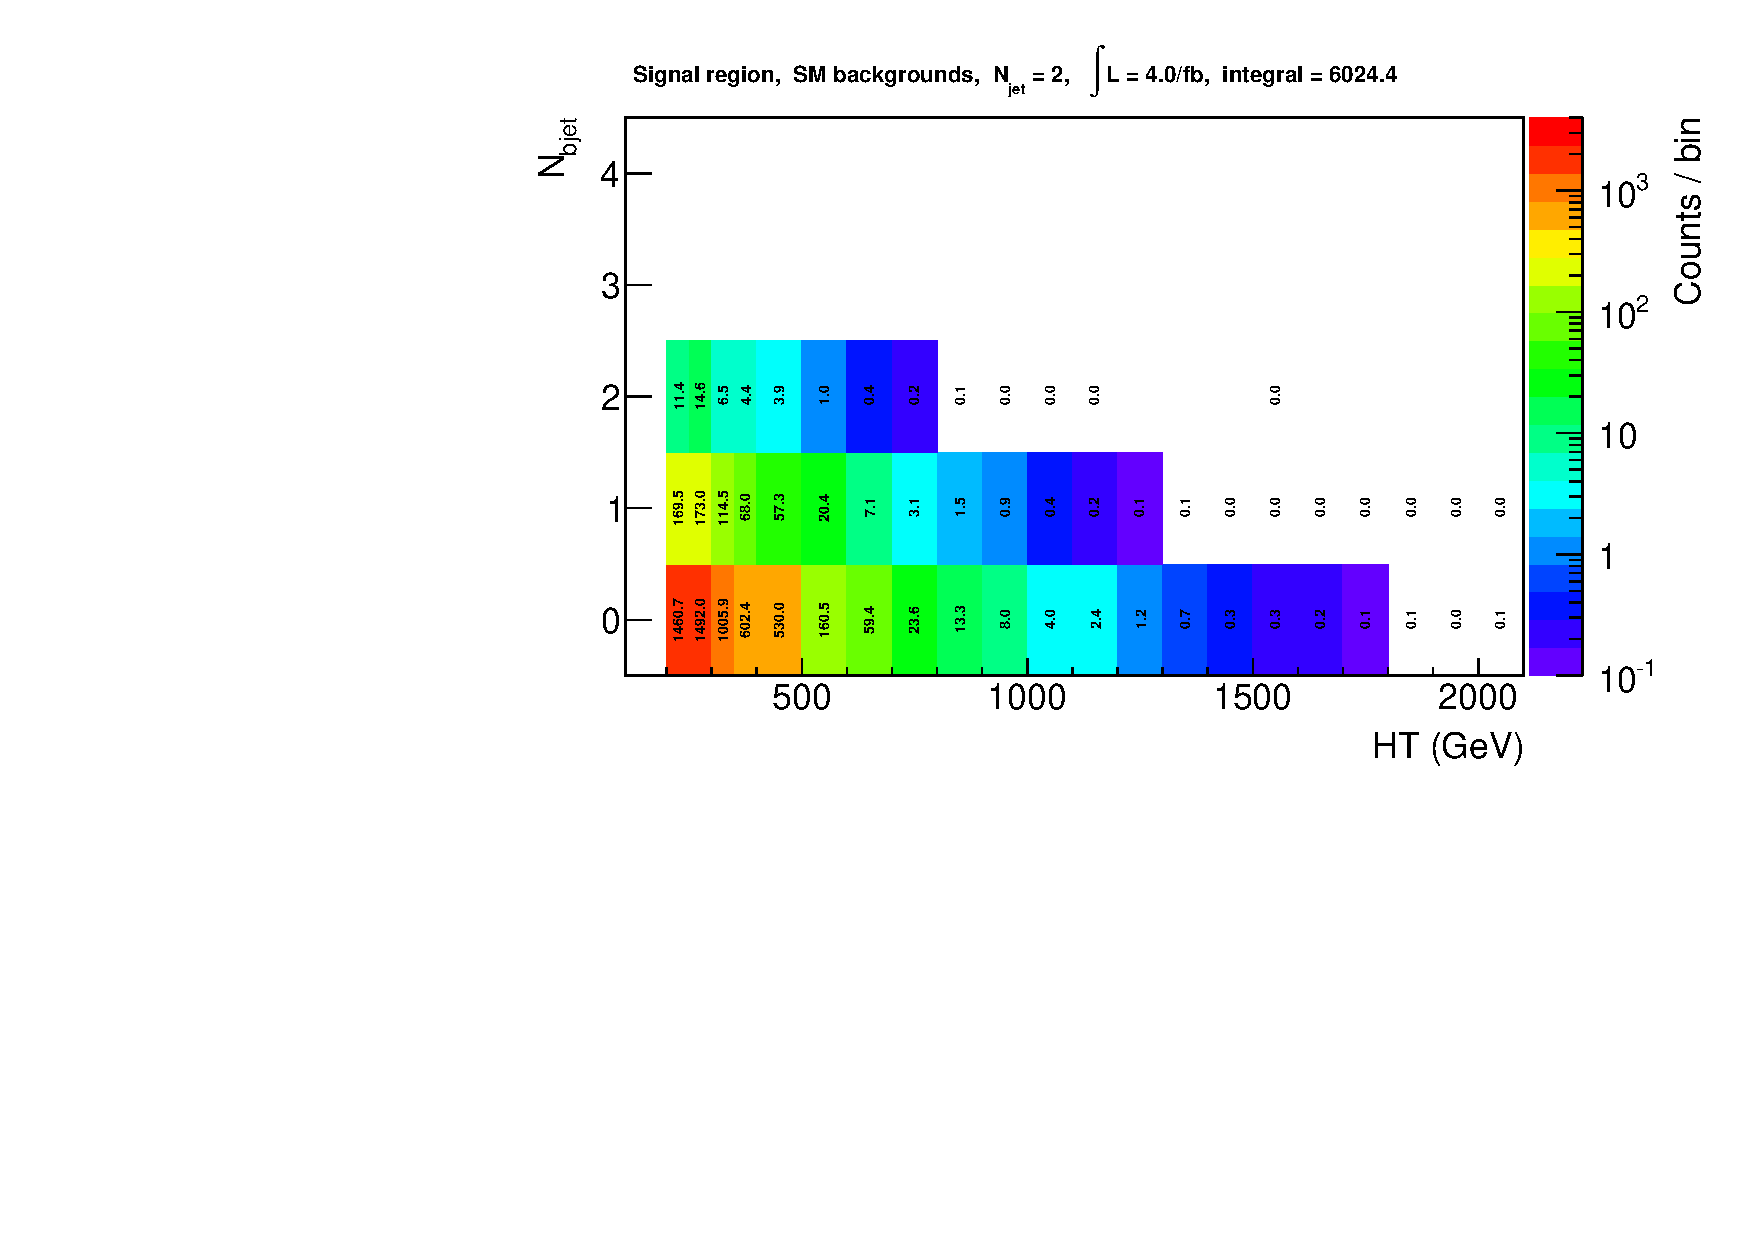
\includegraphics[width=0.5\textwidth]{figures/yieldPlots/had_ewk_eq2j.pdf}
  }~~
  \subfigure[Hadronic signal region yields for the \zInv background
  ($\njet = 2$)]{
    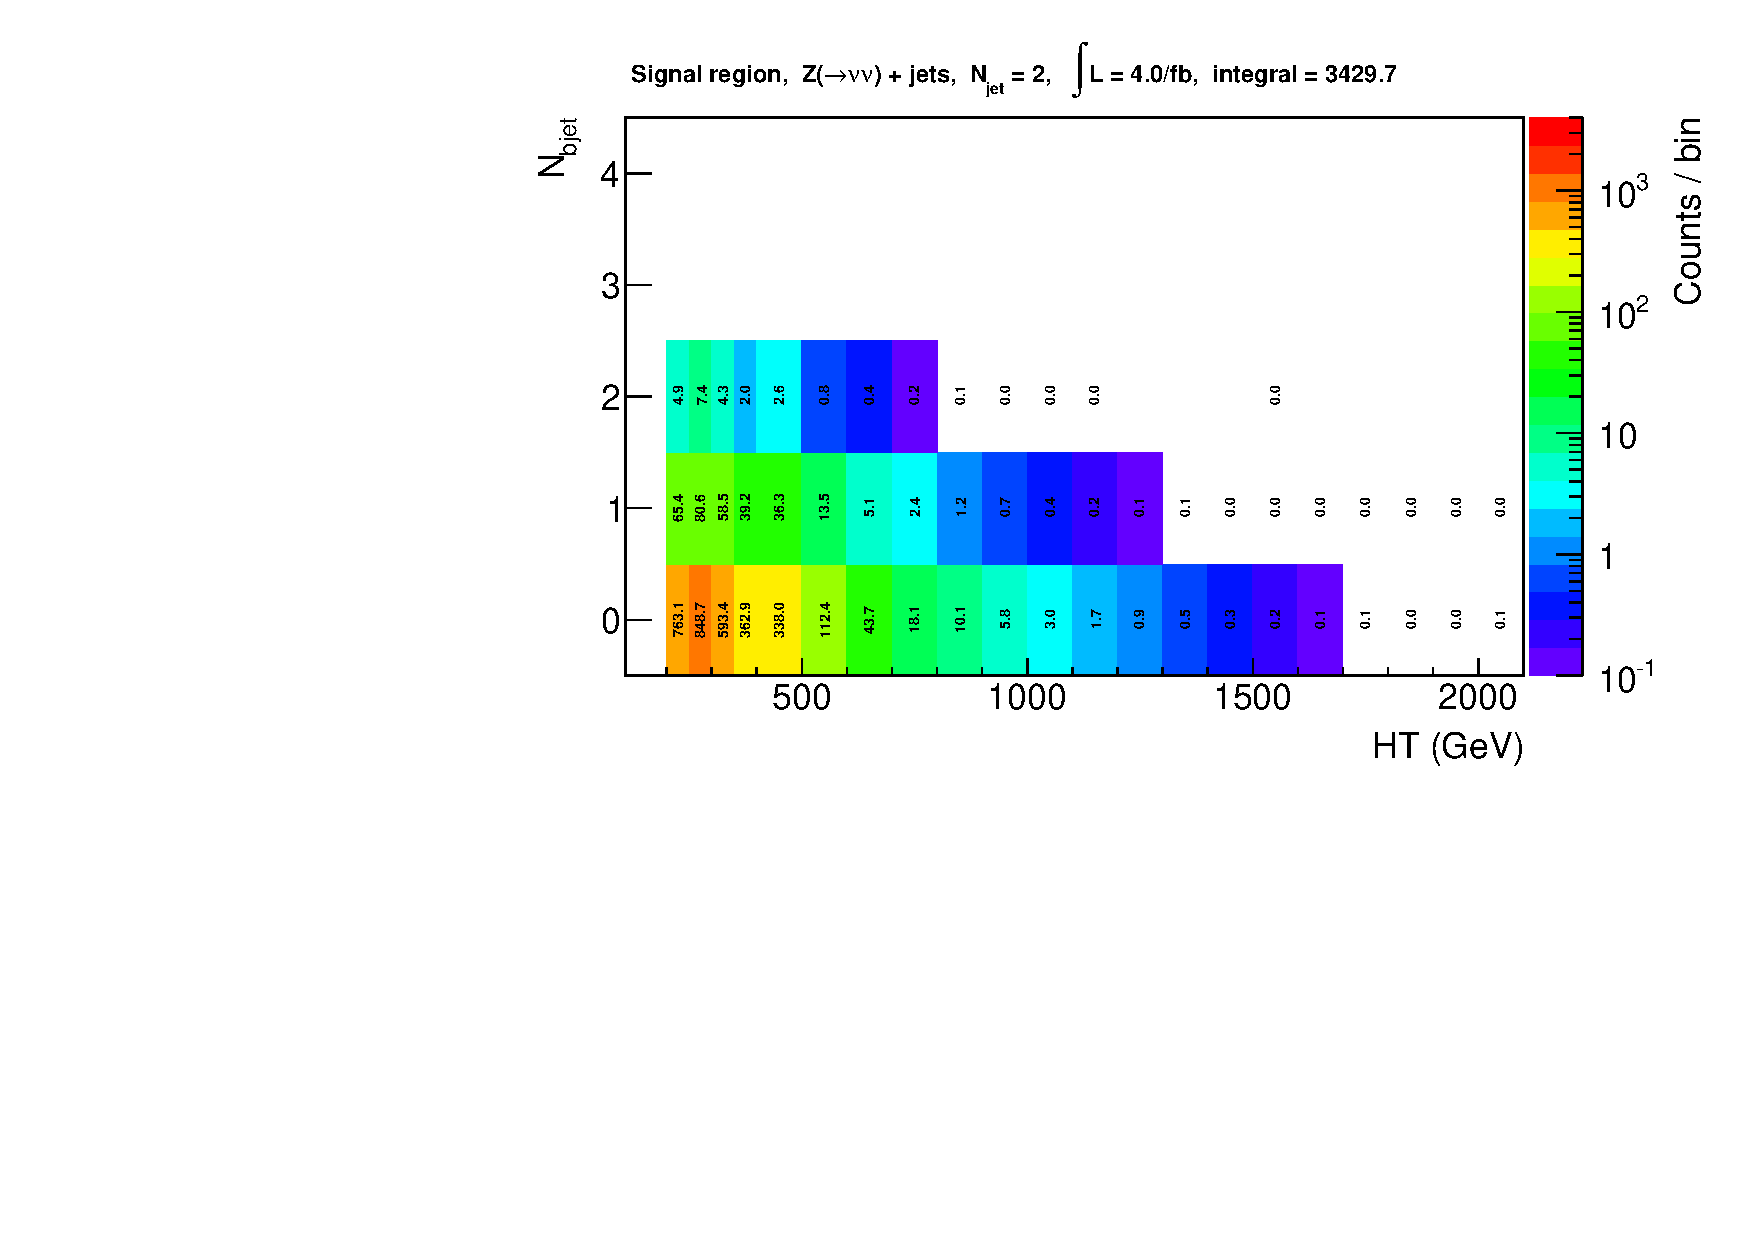
\includegraphics[width=0.5\textwidth]{figures/yieldPlots/had_zinv_eq2j.pdf}
  }\\
  \subfigure[Hadronic signal region yields for W~+~jets backtround
  ($\njet = 2$)]{
    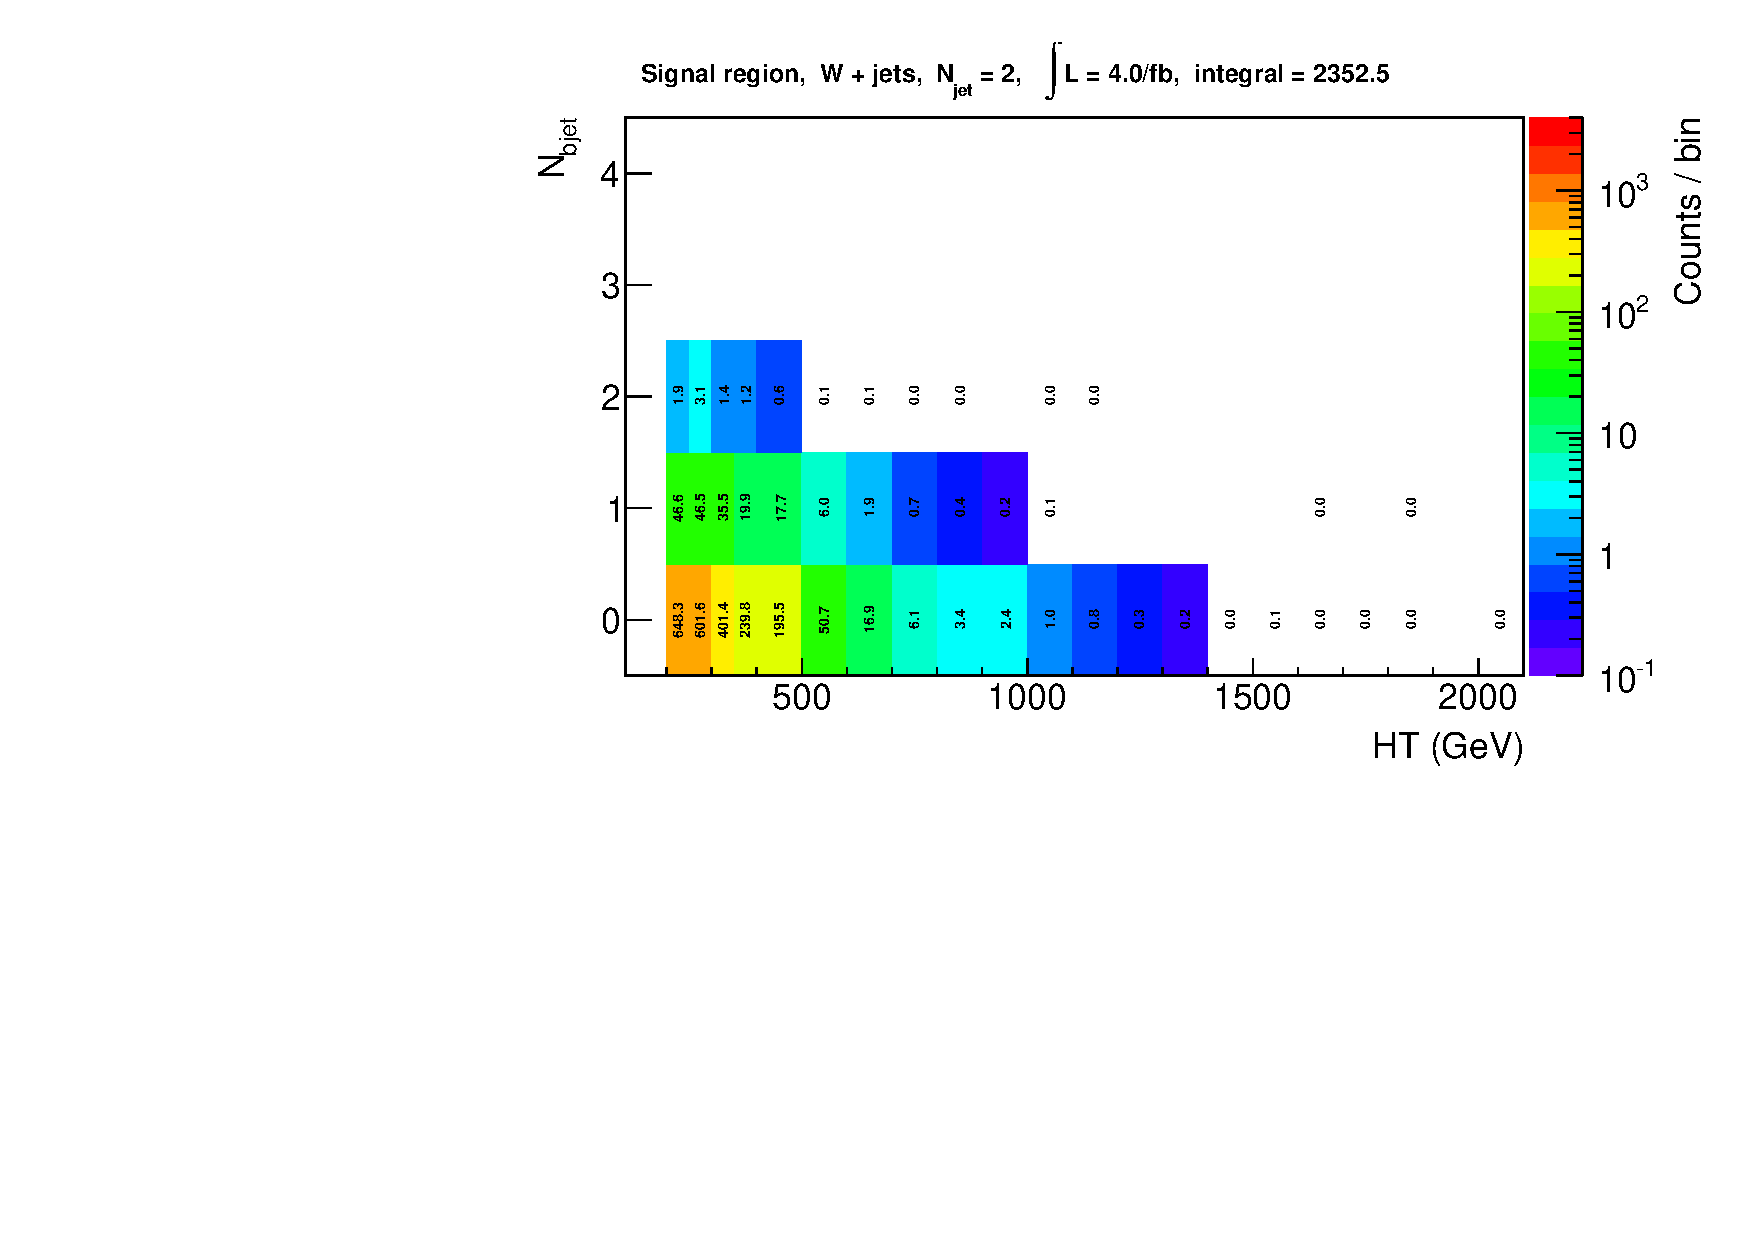
\includegraphics[width=0.5\textwidth]{figures/yieldPlots/had_wjets_eq2j.pdf}
  }~~
  \subfigure[Hadronic signal region yields for \ttbar background
  ($\njet = 2$)]{
    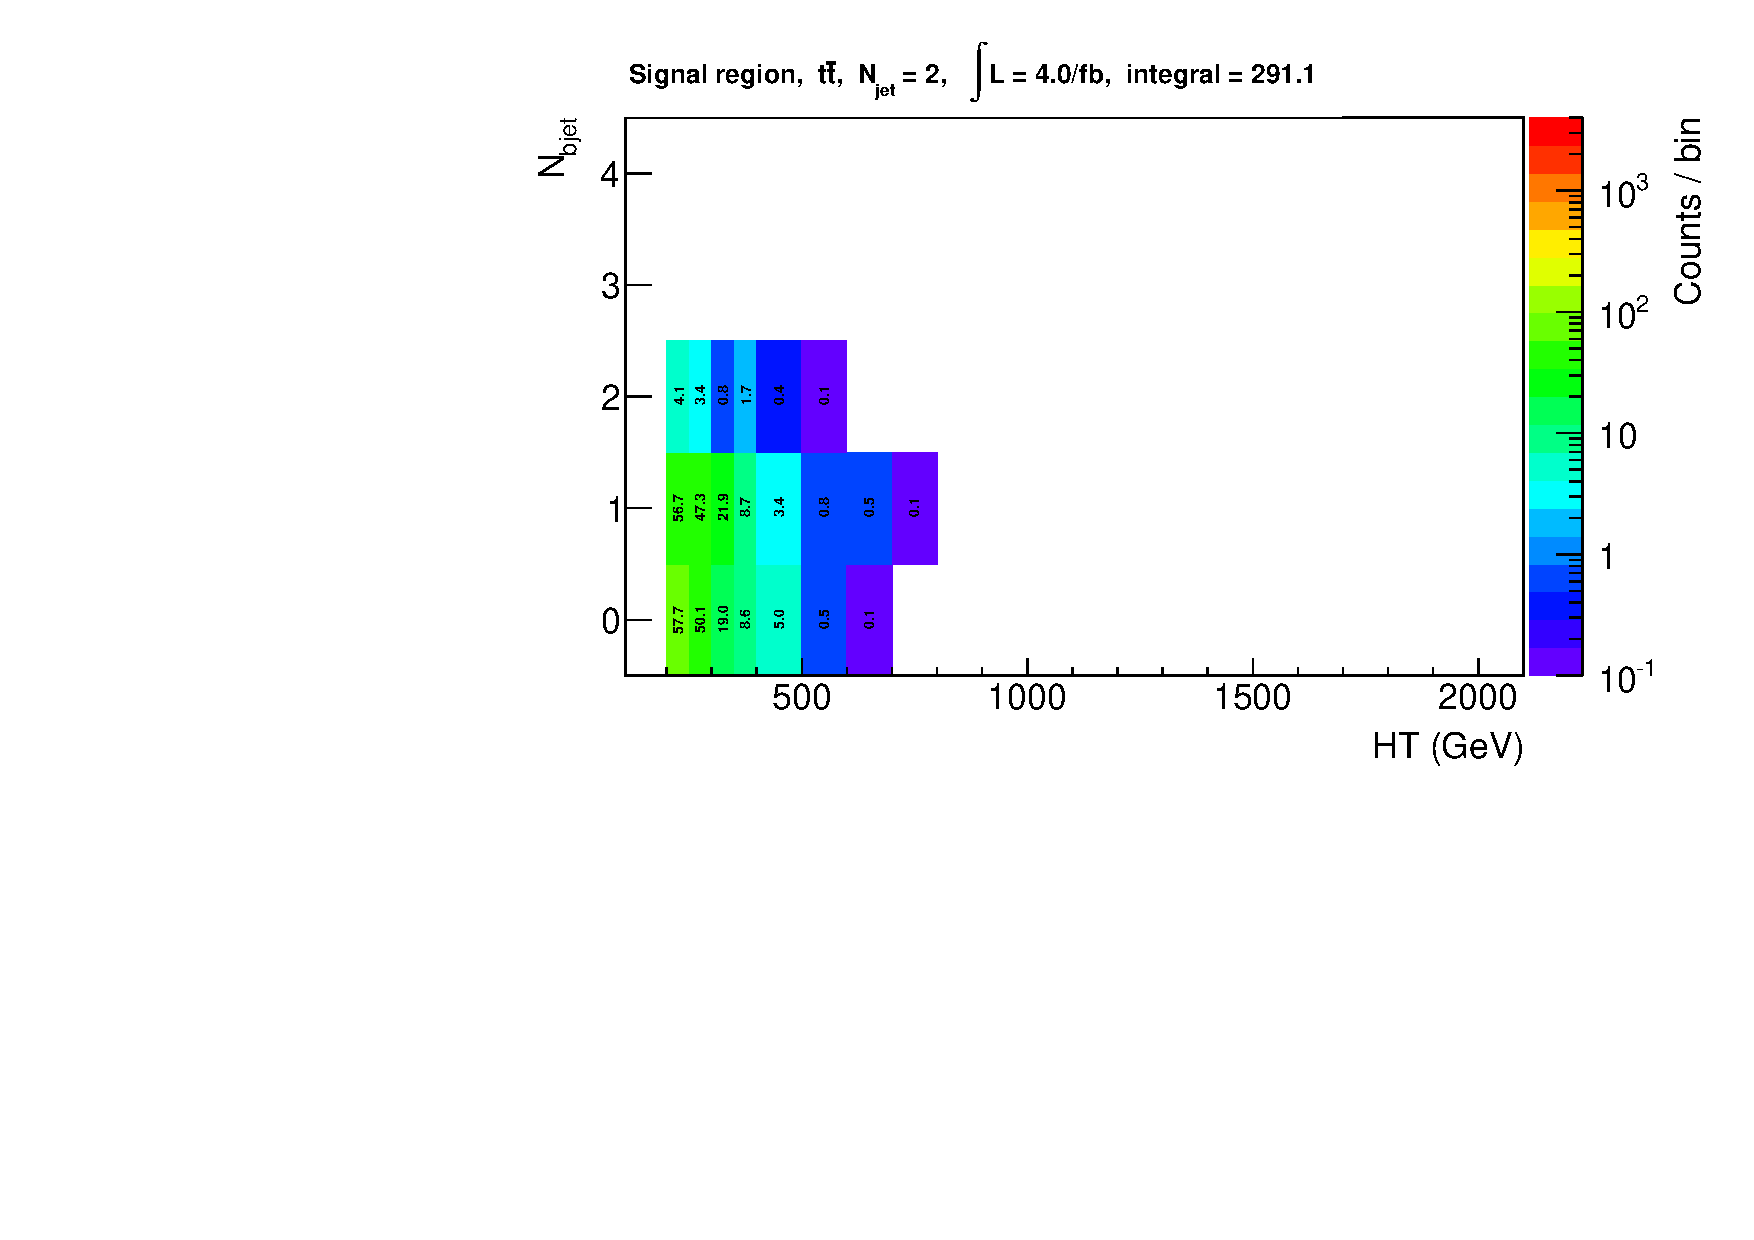
\includegraphics[width=0.5\textwidth]{figures/yieldPlots/had_ttbar_eq2j.pdf}
  }
  \caption{\label{fig:ewkYields1} Yields at $4\fbinv$ for the electroweak backgrounds in the
  hadronic signal region, $\njet=2$. The binning is chosen to be in line with the analysis
  bins. The contribution from the dominant backgrounds is shown separately.}
\end{figure}
\begin{figure}[]
  \centering
  \subfigure[Hadronic signal region yields for electroweak backgrounds
  ($\njet = 3$)]{
    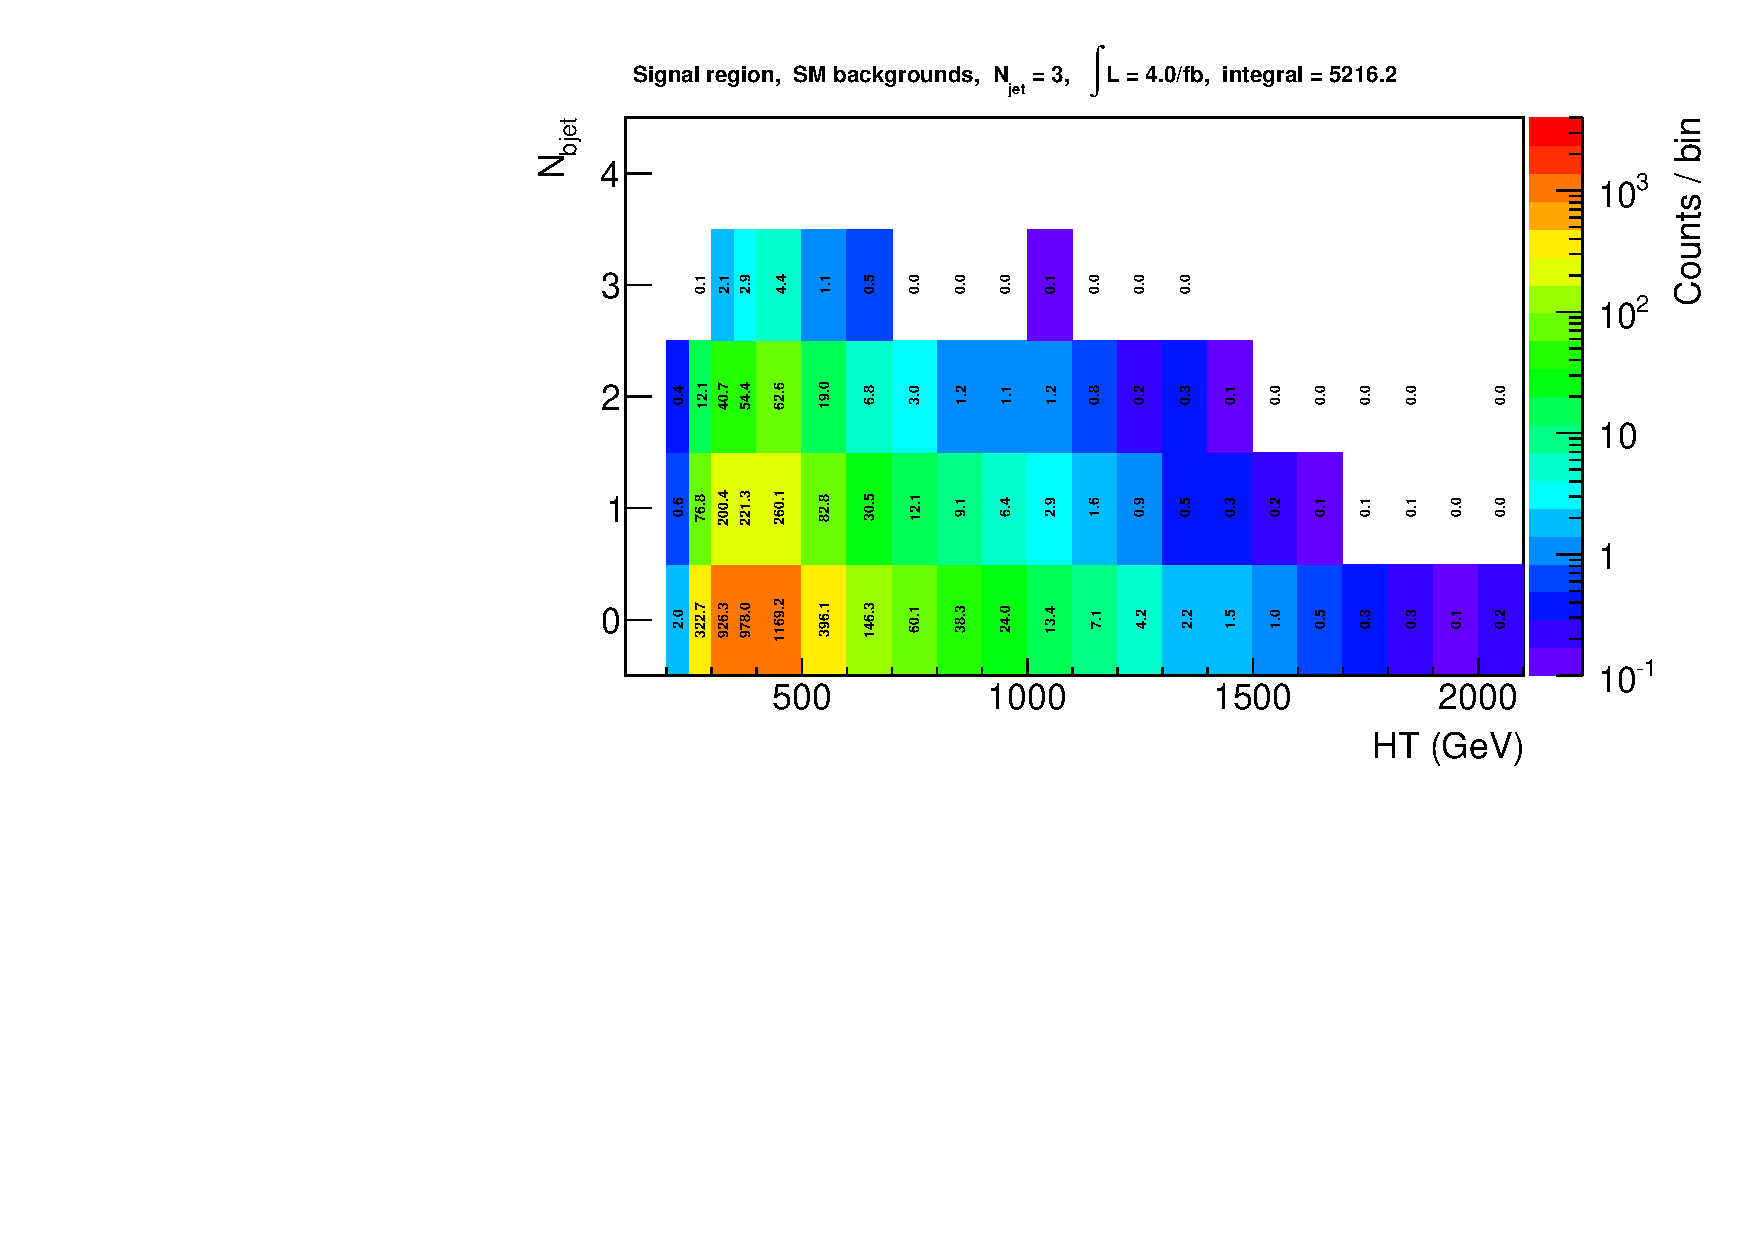
\includegraphics[width=0.5\textwidth]{figures/yieldPlots/had_ewk_eq3j.pdf}
  }~~
  \subfigure[Hadronic signal region yields for the \zInv background
  ($\njet = 3$)]{
    \includegraphics[width=0.5\textwidth]{figures/yieldPlots/had_zInv_eq3j.pdf}
  }\\
  \subfigure[Hadronic signal region yields for W~+~jets backtround
  ($\njet = 3$)]{
    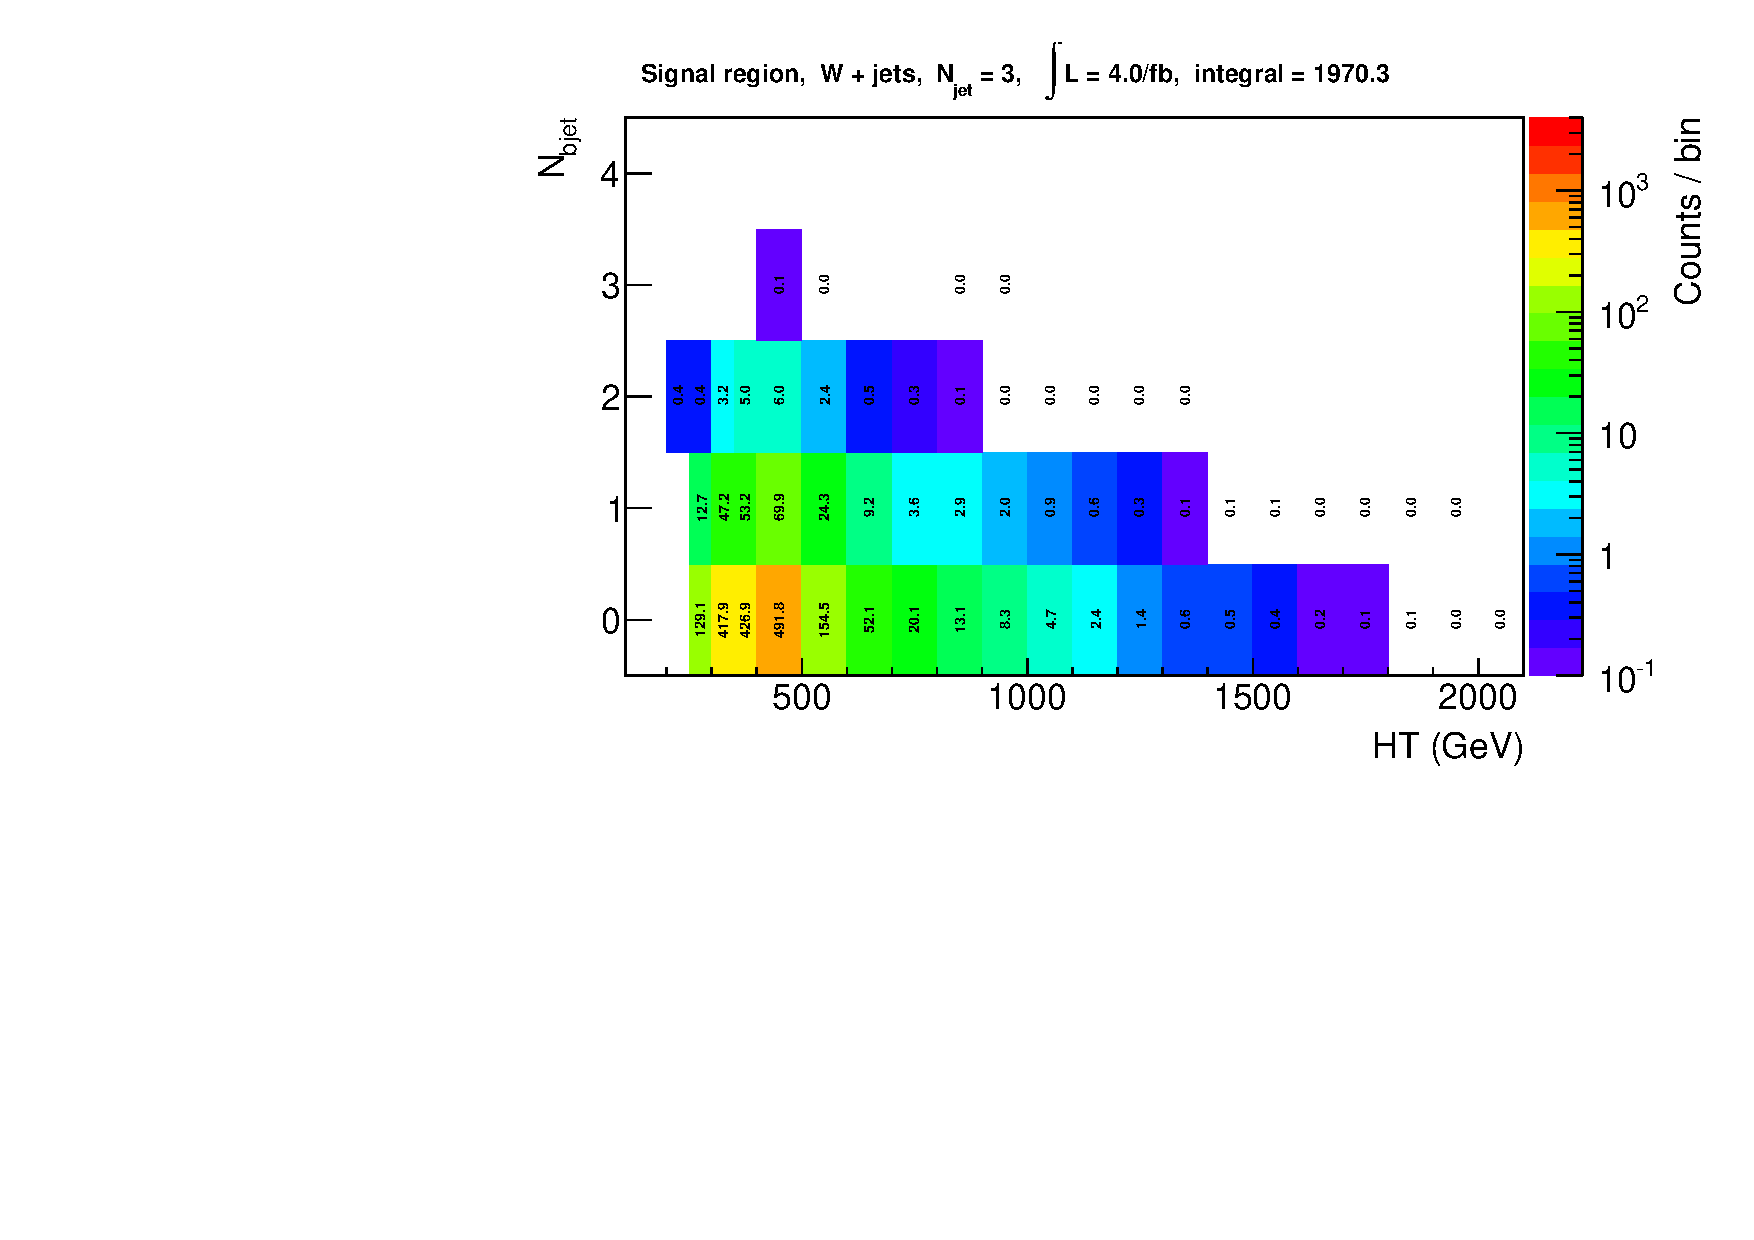
\includegraphics[width=0.5\textwidth]{figures/yieldPlots/had_wjets_eq3j.pdf}
  }~~
  \subfigure[Hadronic signal region yields for \ttbar background
  ($\njet = 3$)]{
    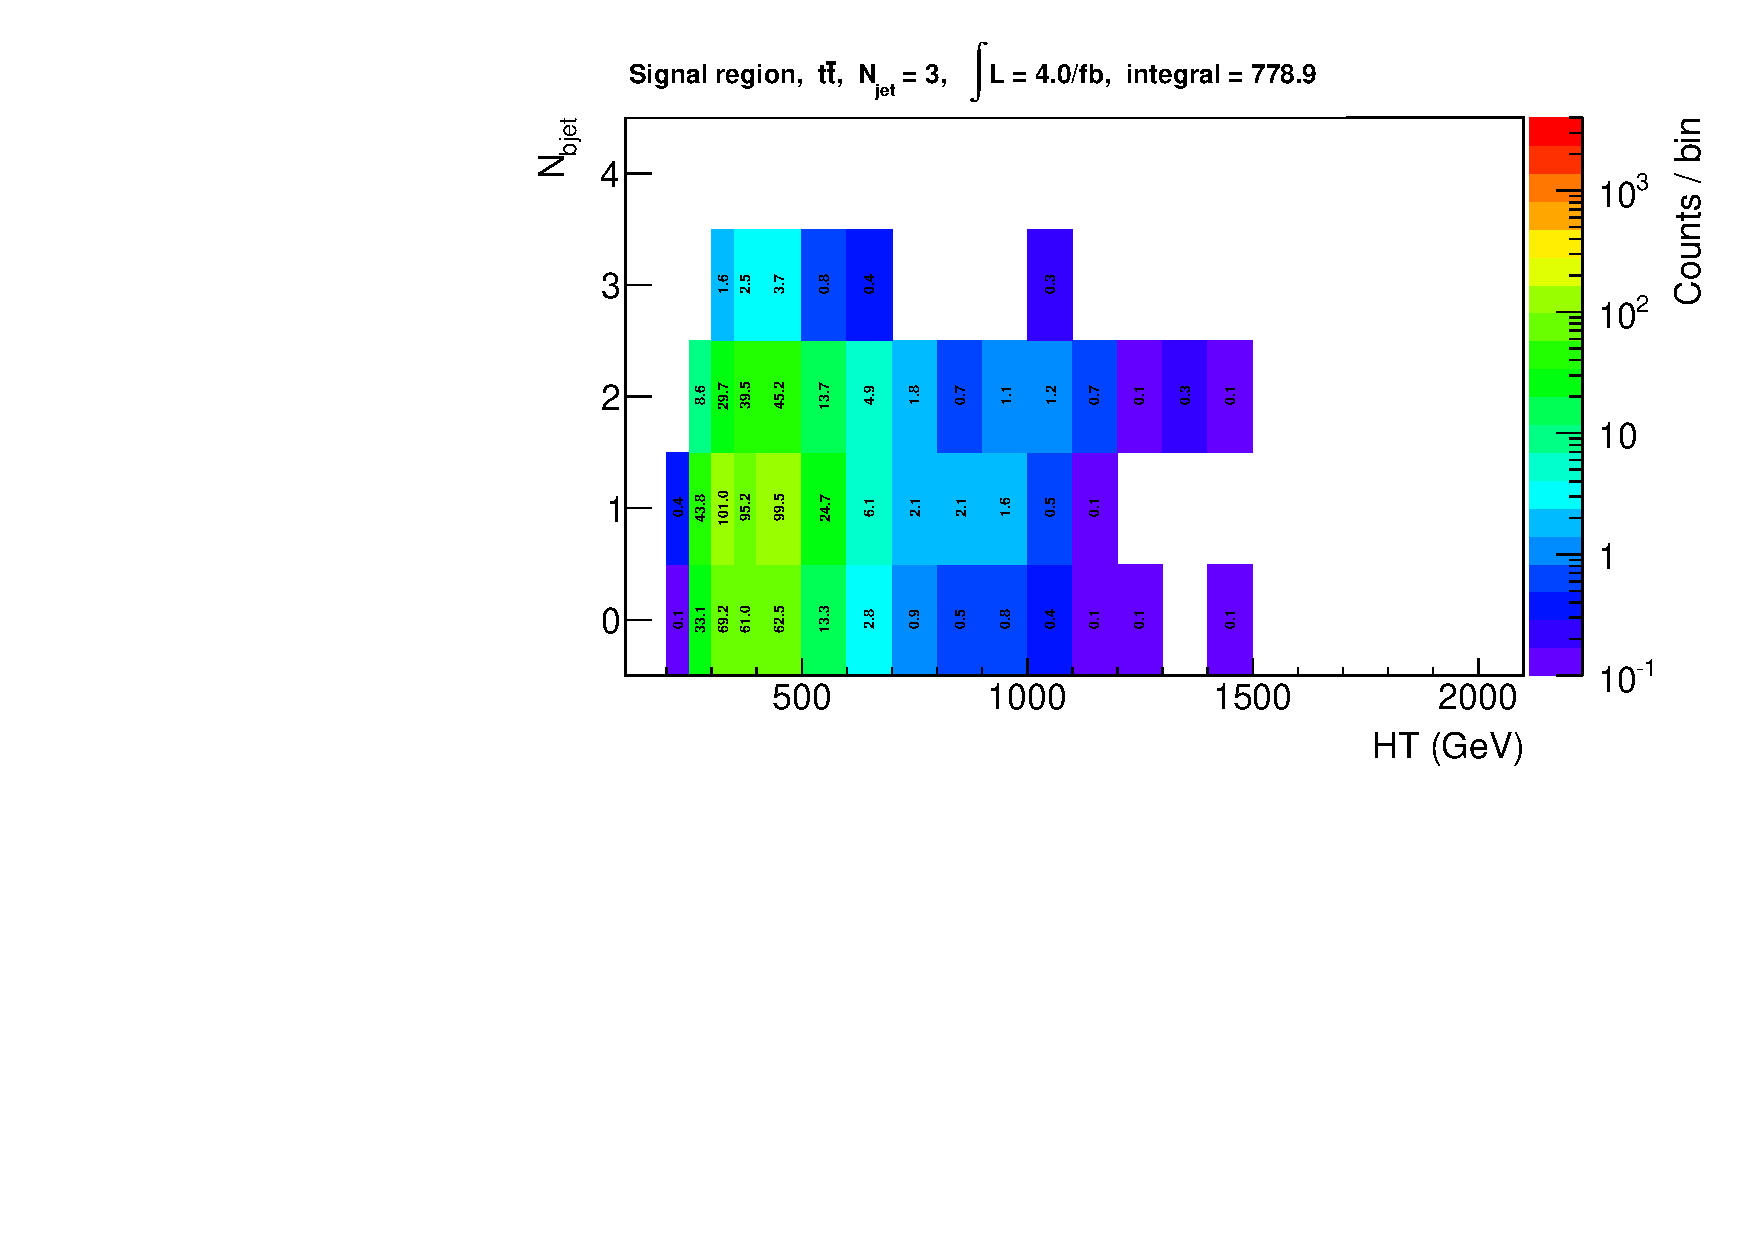
\includegraphics[width=0.5\textwidth]{figures/yieldPlots/had_ttbar_eq3j.pdf}
  }
  \caption{\label{fig:ewkYields2} Yields at $4\fbinv$ for the electroweak backgrounds in the
  hadronic signal region, $\njet=3$. The binning is chosen to be in line with the analysis
  bins. The contribution from the dominant backgrounds is shown separately.}
\end{figure}
\begin{figure}[]
  \centering
  \subfigure[Hadronic signal region yields for electroweak backgrounds
  ($\njet = 4$)]{
    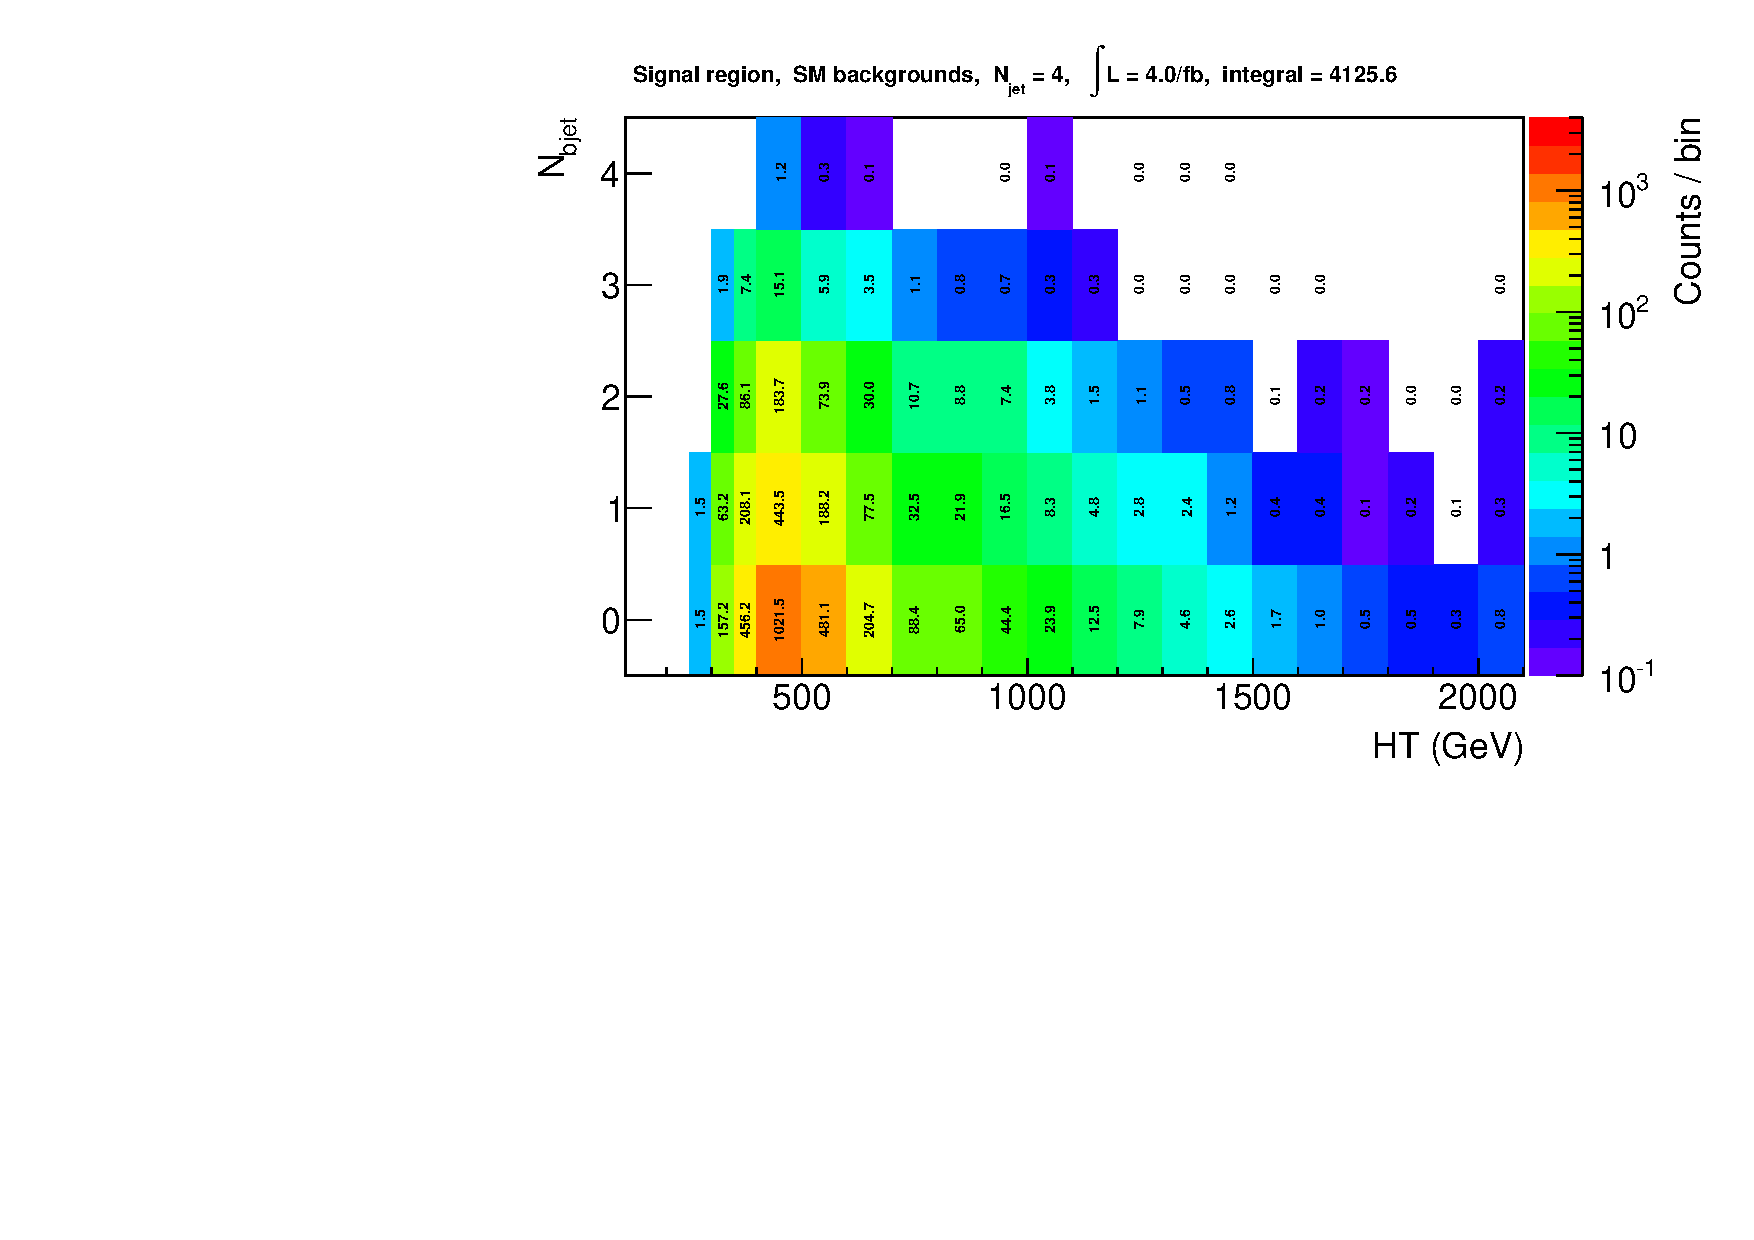
\includegraphics[width=0.5\textwidth]{figures/yieldPlots/had_ewk_eq4j.pdf}
  }~~
  \subfigure[Hadronic signal region yields for the \zInv background
  ($\njet = 4$)]{
    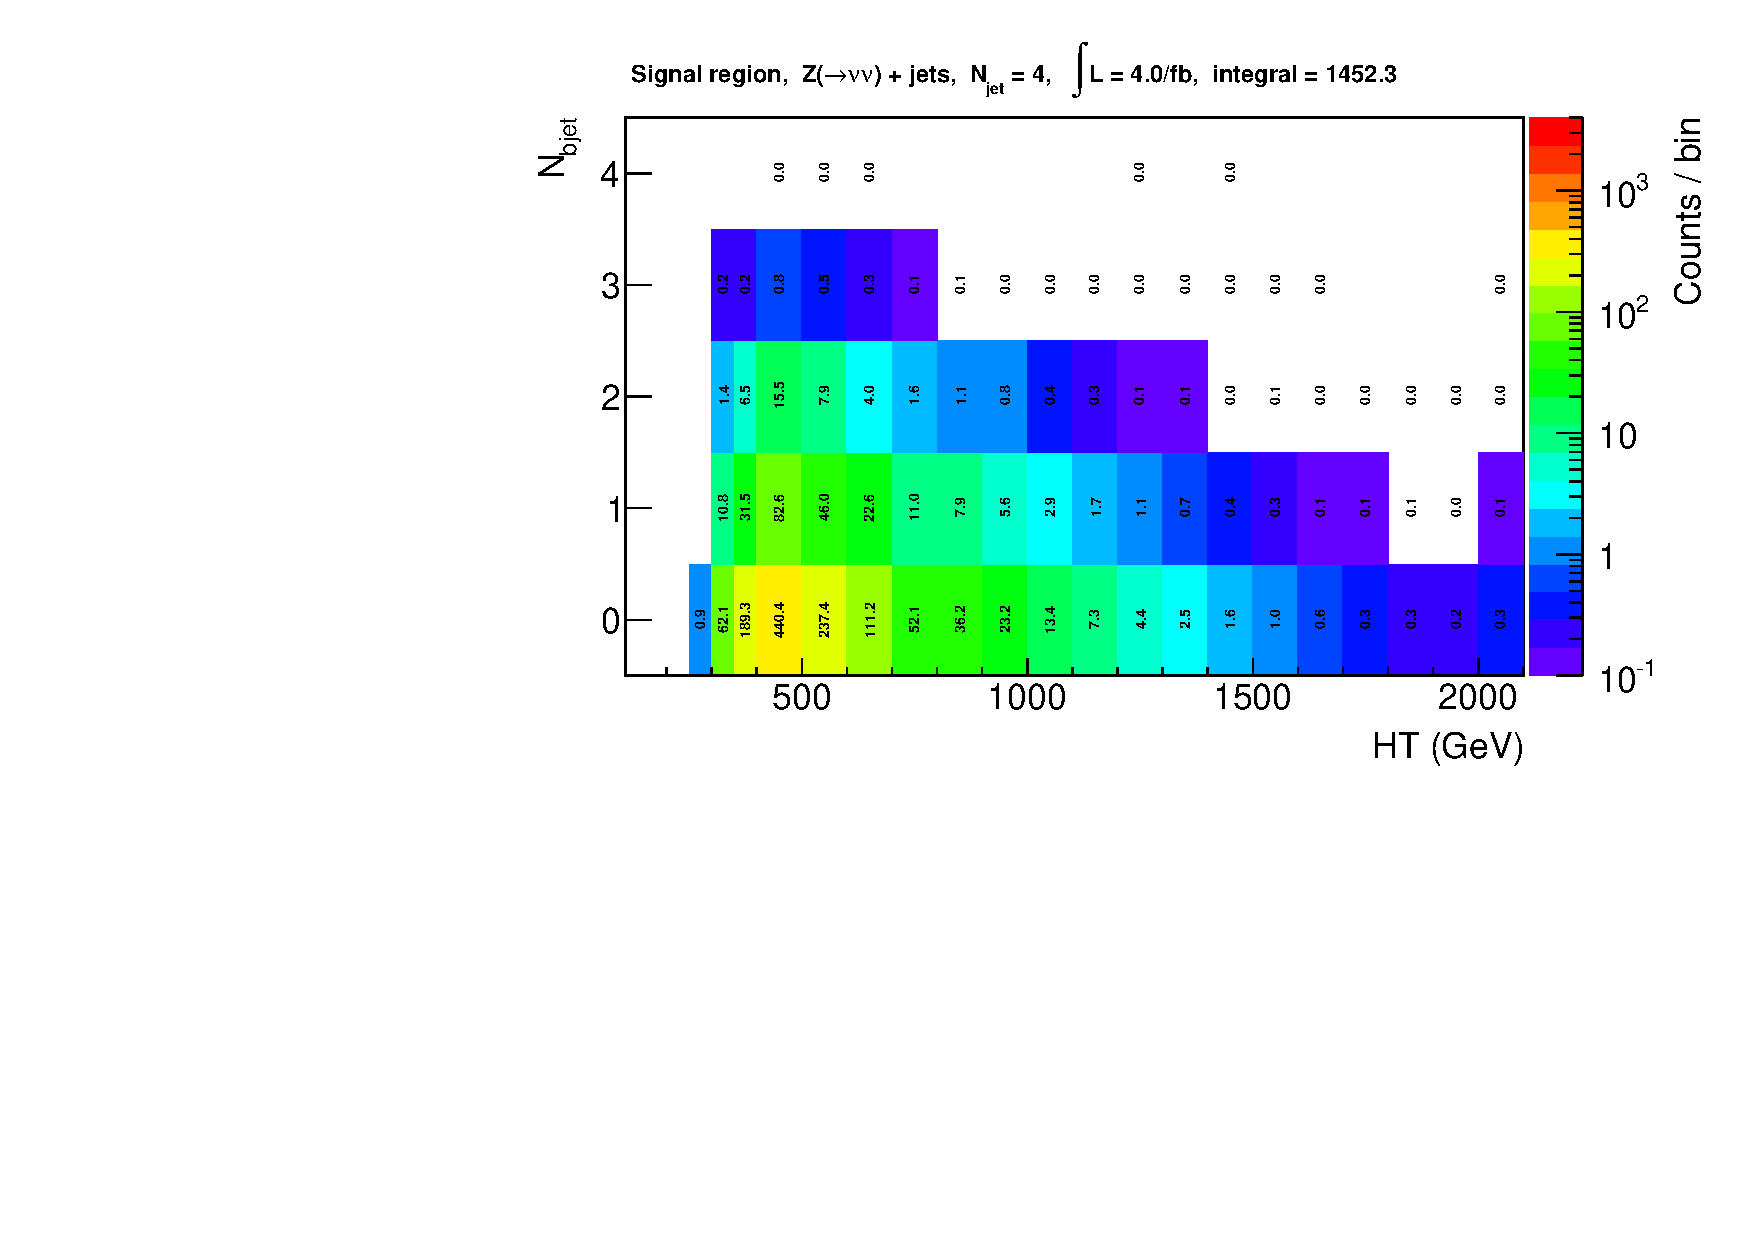
\includegraphics[width=0.5\textwidth]{figures/yieldPlots/had_zinv_eq4j.pdf}
  }\\
  \subfigure[Hadronic signal region yields for W~+~jets backtround
  ($\njet = 4$)]{
    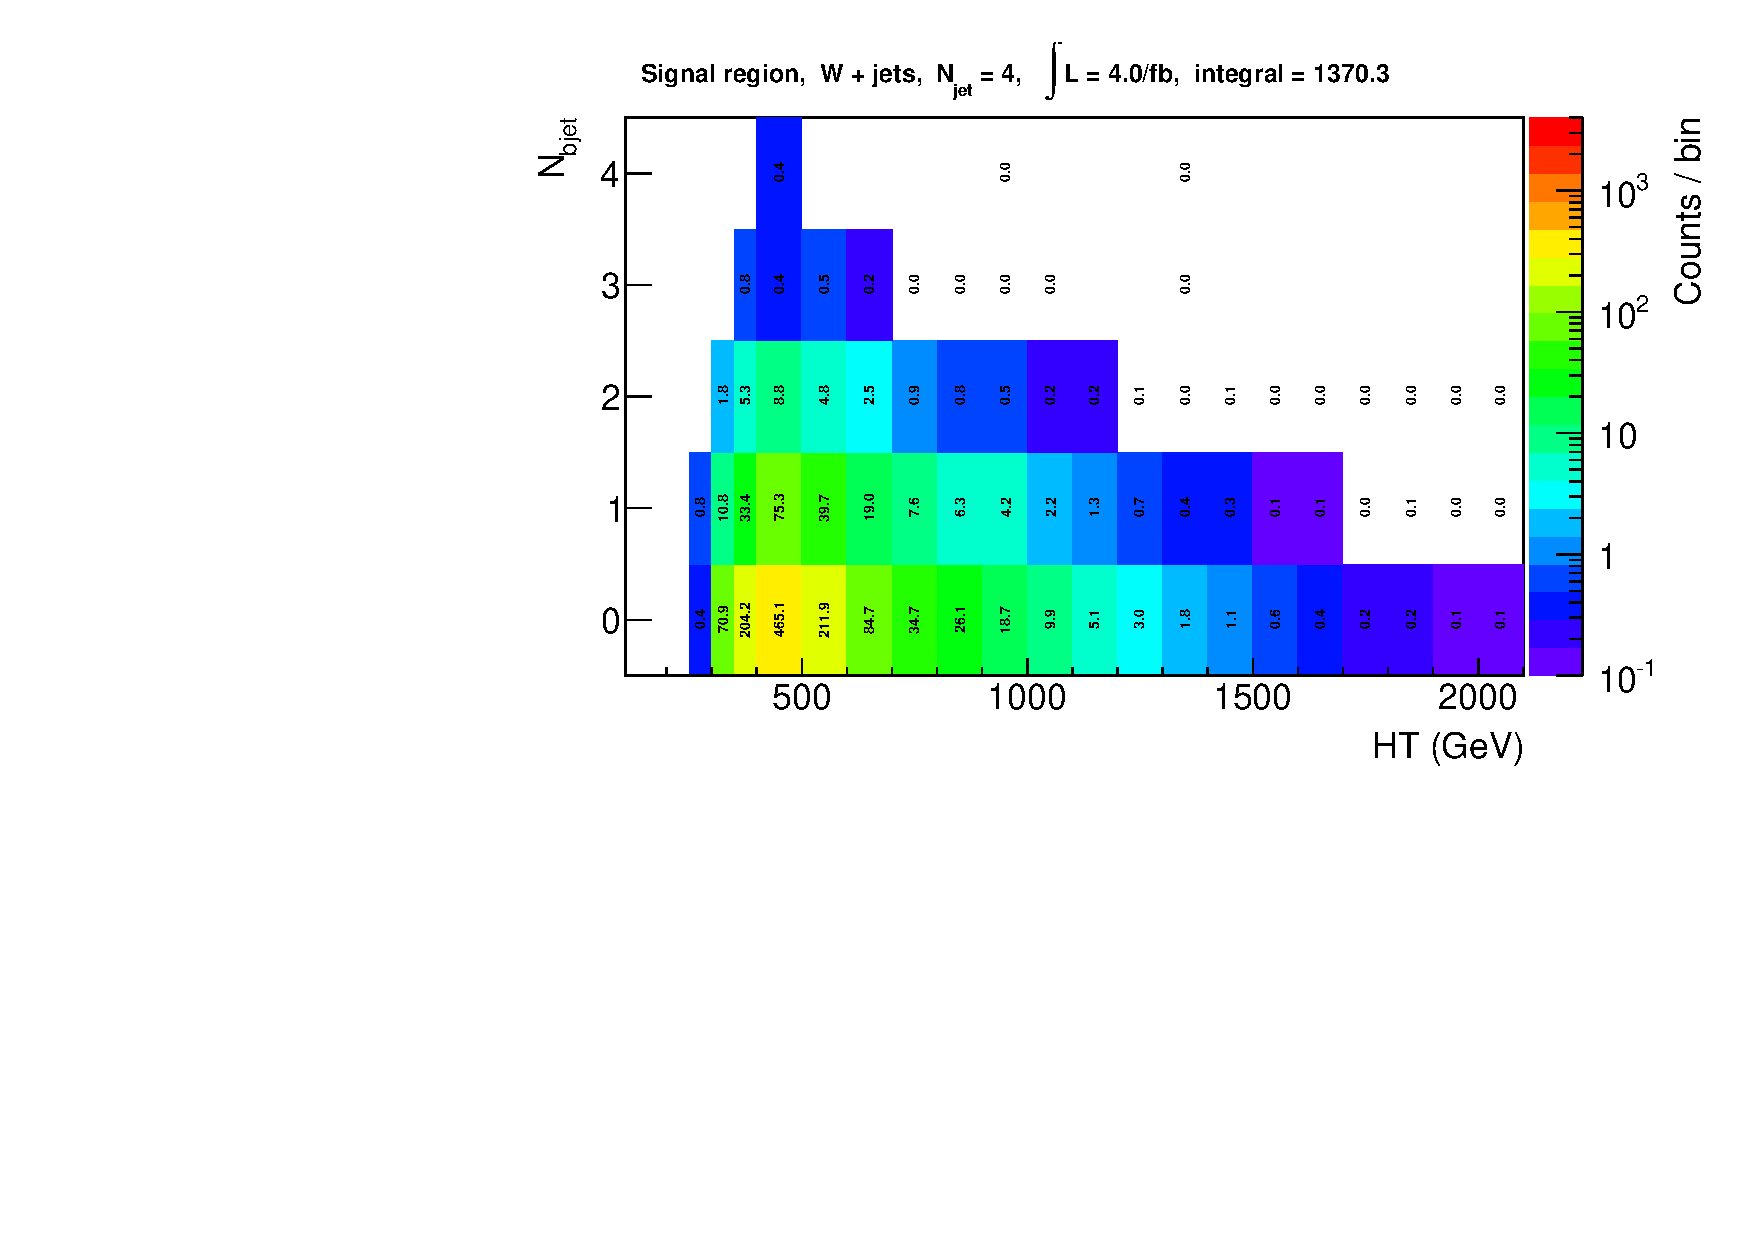
\includegraphics[width=0.5\textwidth]{figures/yieldPlots/had_wjets_eq4j.pdf}
  }~~
  \subfigure[Hadronic signal region yields for \ttbar background
  ($\njet = 4$)]{
    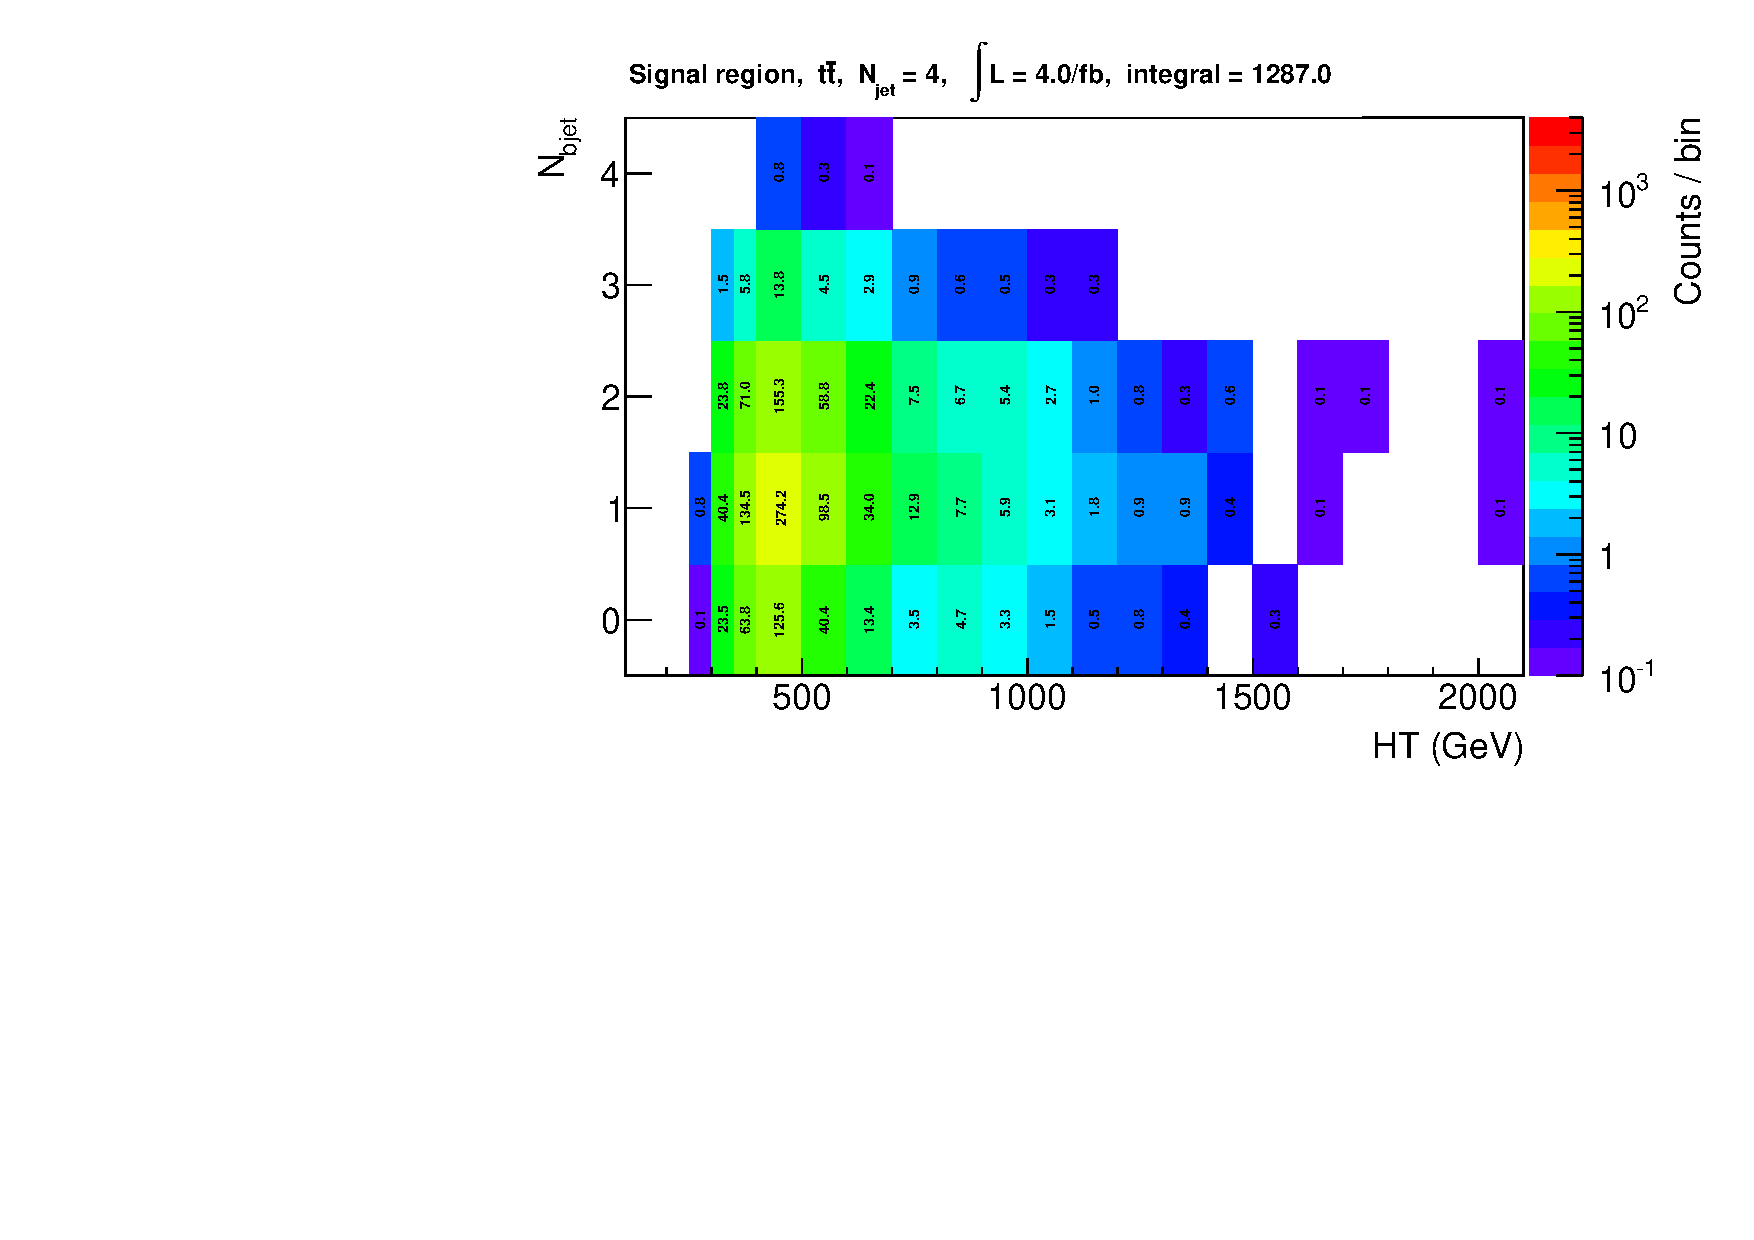
\includegraphics[width=0.5\textwidth]{figures/yieldPlots/had_ttbar_eq4j.pdf}
  }
  \caption{\label{fig:ewkYields3} Yields at $4\fbinv$ for the electroweak backgrounds in the
  hadronic signal region, $\njet=4$. The binning is chosen to be in line with the analysis
  bins. The contribution from the dominant backgrounds is shown separately.}
\end{figure}
\begin{figure}[]
  \centering
  \subfigure[Hadronic signal region yields for electroweak backgrounds
  ($\njet \geq 5$)]{
    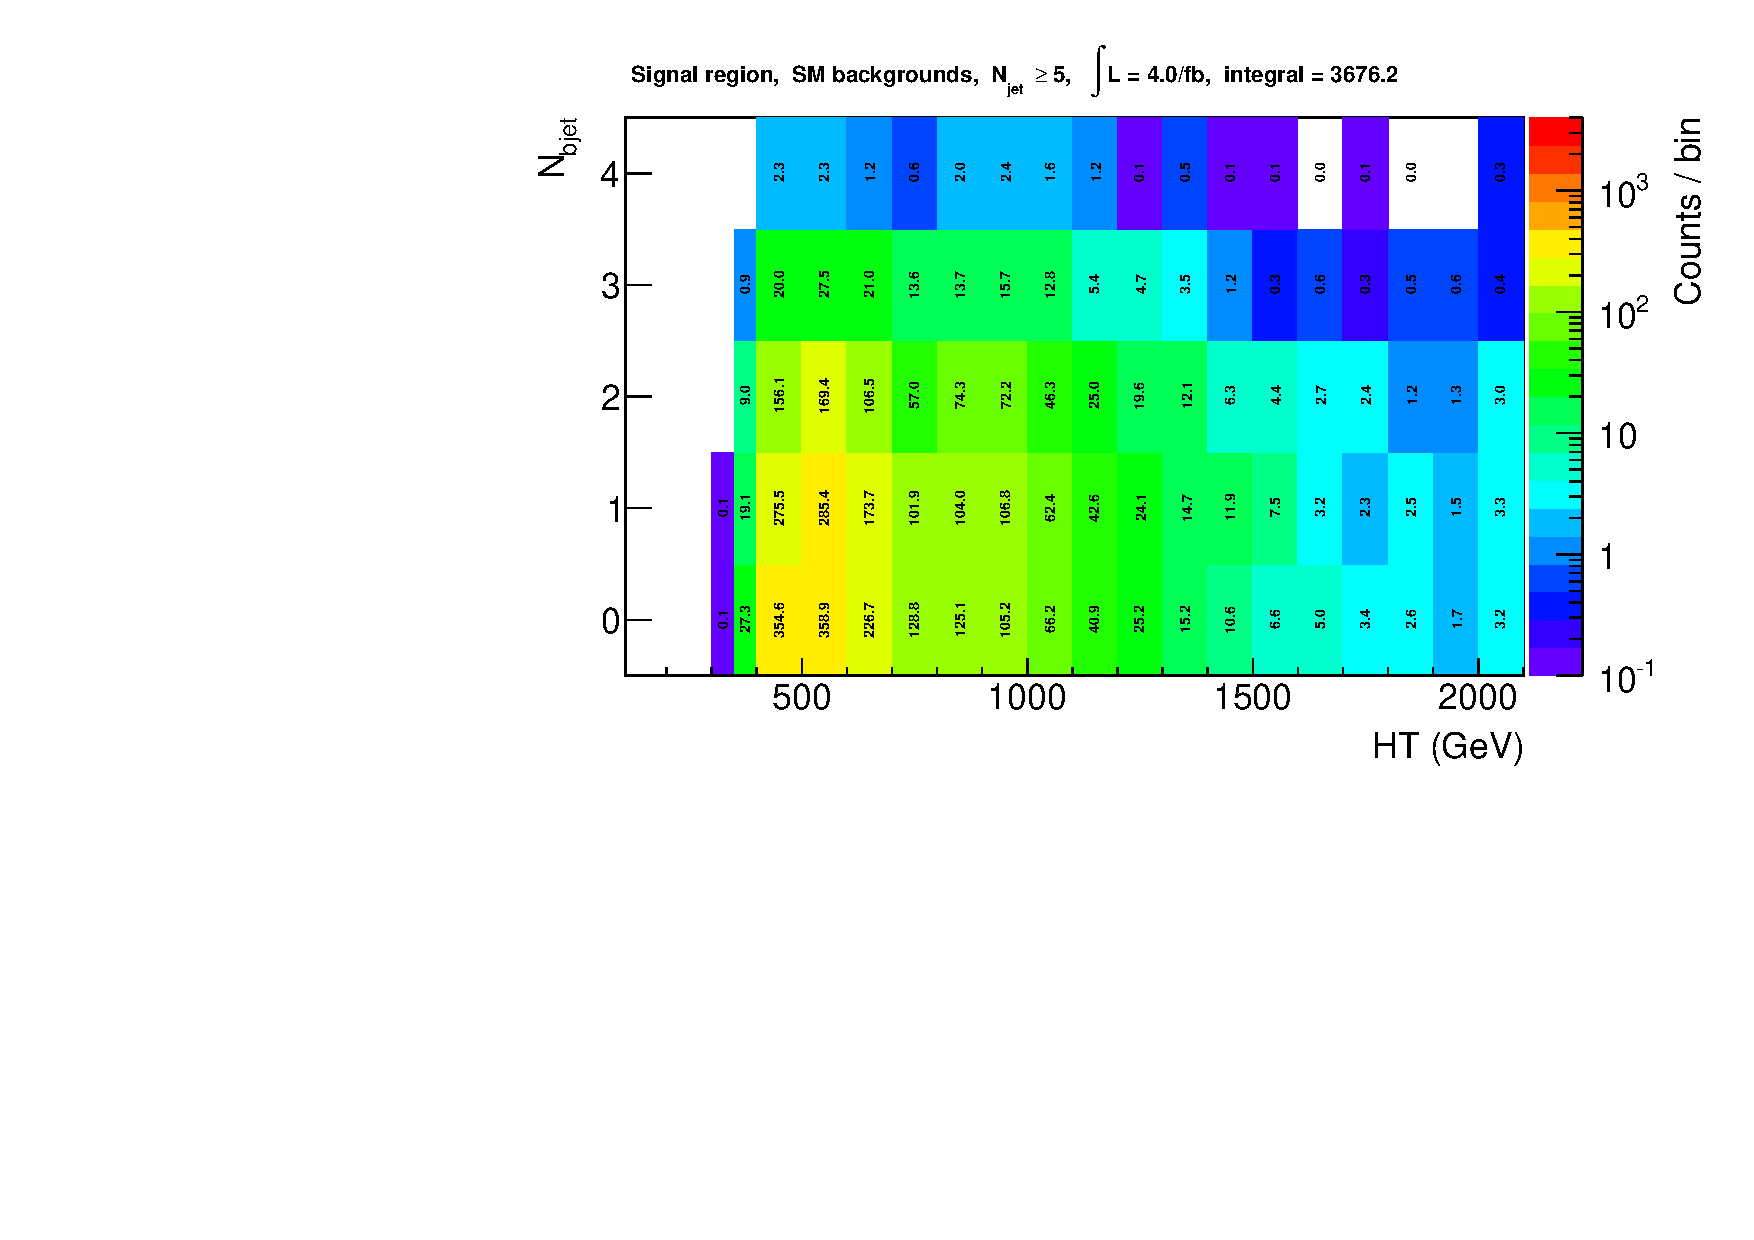
\includegraphics[width=0.5\textwidth]{figures/yieldPlots/had_ewk_ge5j.pdf}
  } ~~
  \subfigure[Hadronic signal region yields for the \zInv background
  ($\njet \geq 5$)]{
    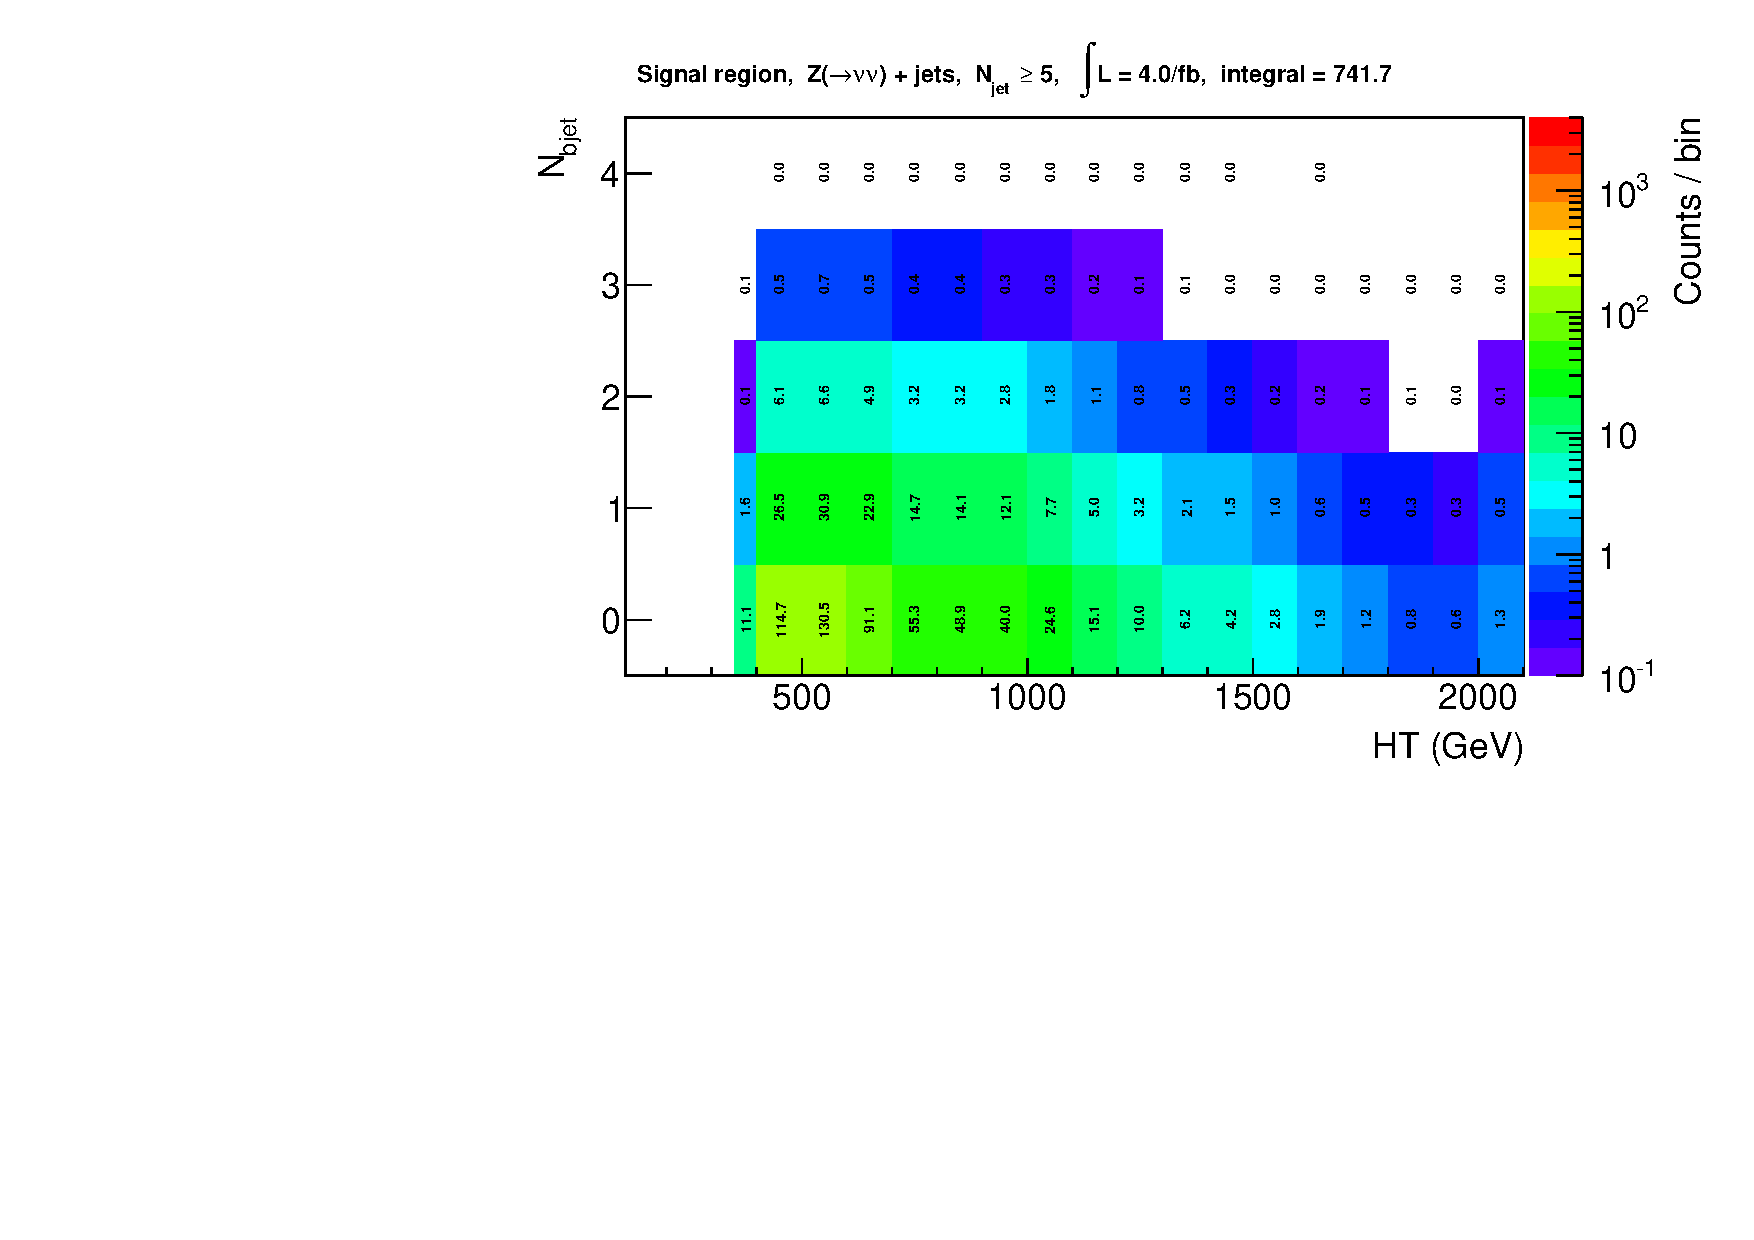
\includegraphics[width=0.5\textwidth]{figures/yieldPlots/had_zinv_ge5j.pdf}
  }\\
  \subfigure[Hadronic signal region yields for W~+~jets backtround
  ($\njet \geq 5$)]{
    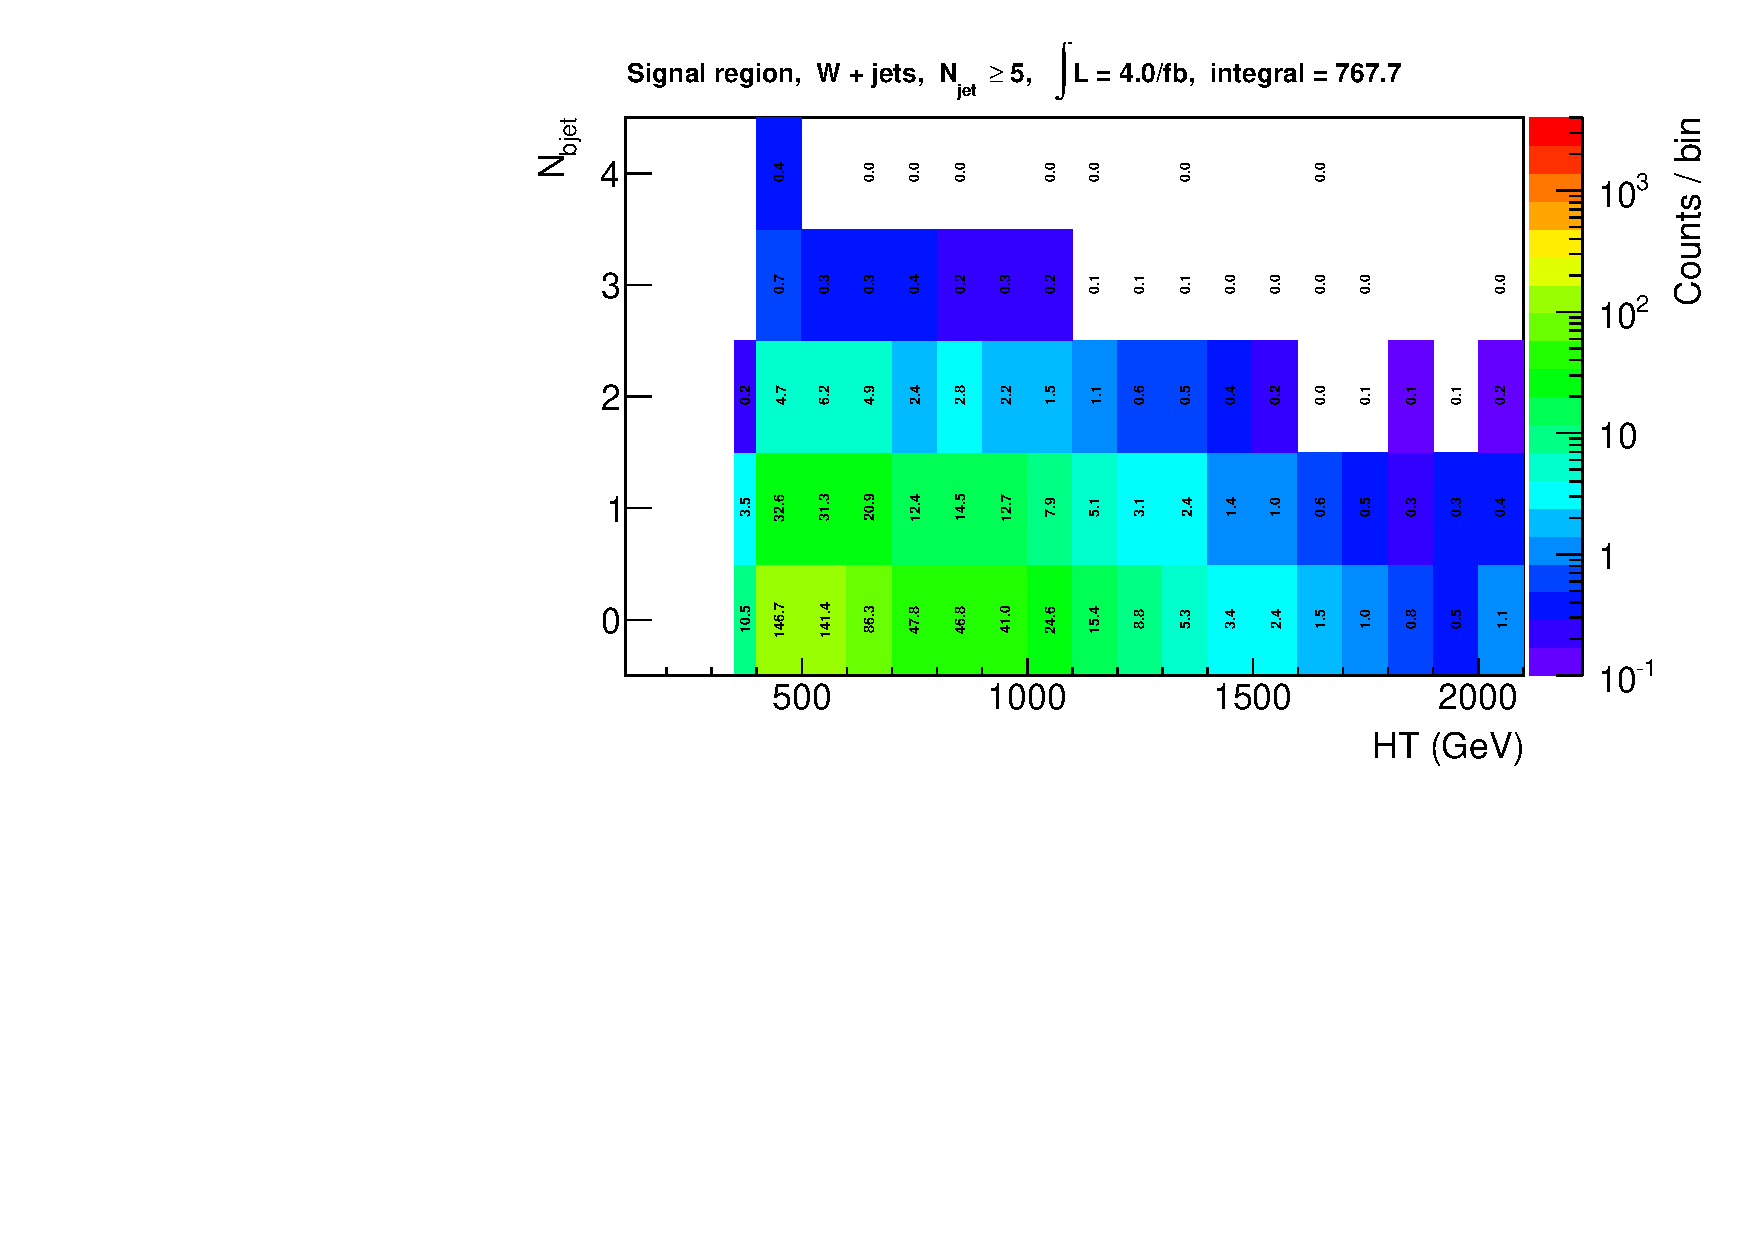
\includegraphics[width=0.5\textwidth]{figures/yieldPlots/had_wjets_ge5j.pdf}
  }~~
  \subfigure[Hadronic signal region yields for \ttbar background
  ($\njet \geq 5$)]{
    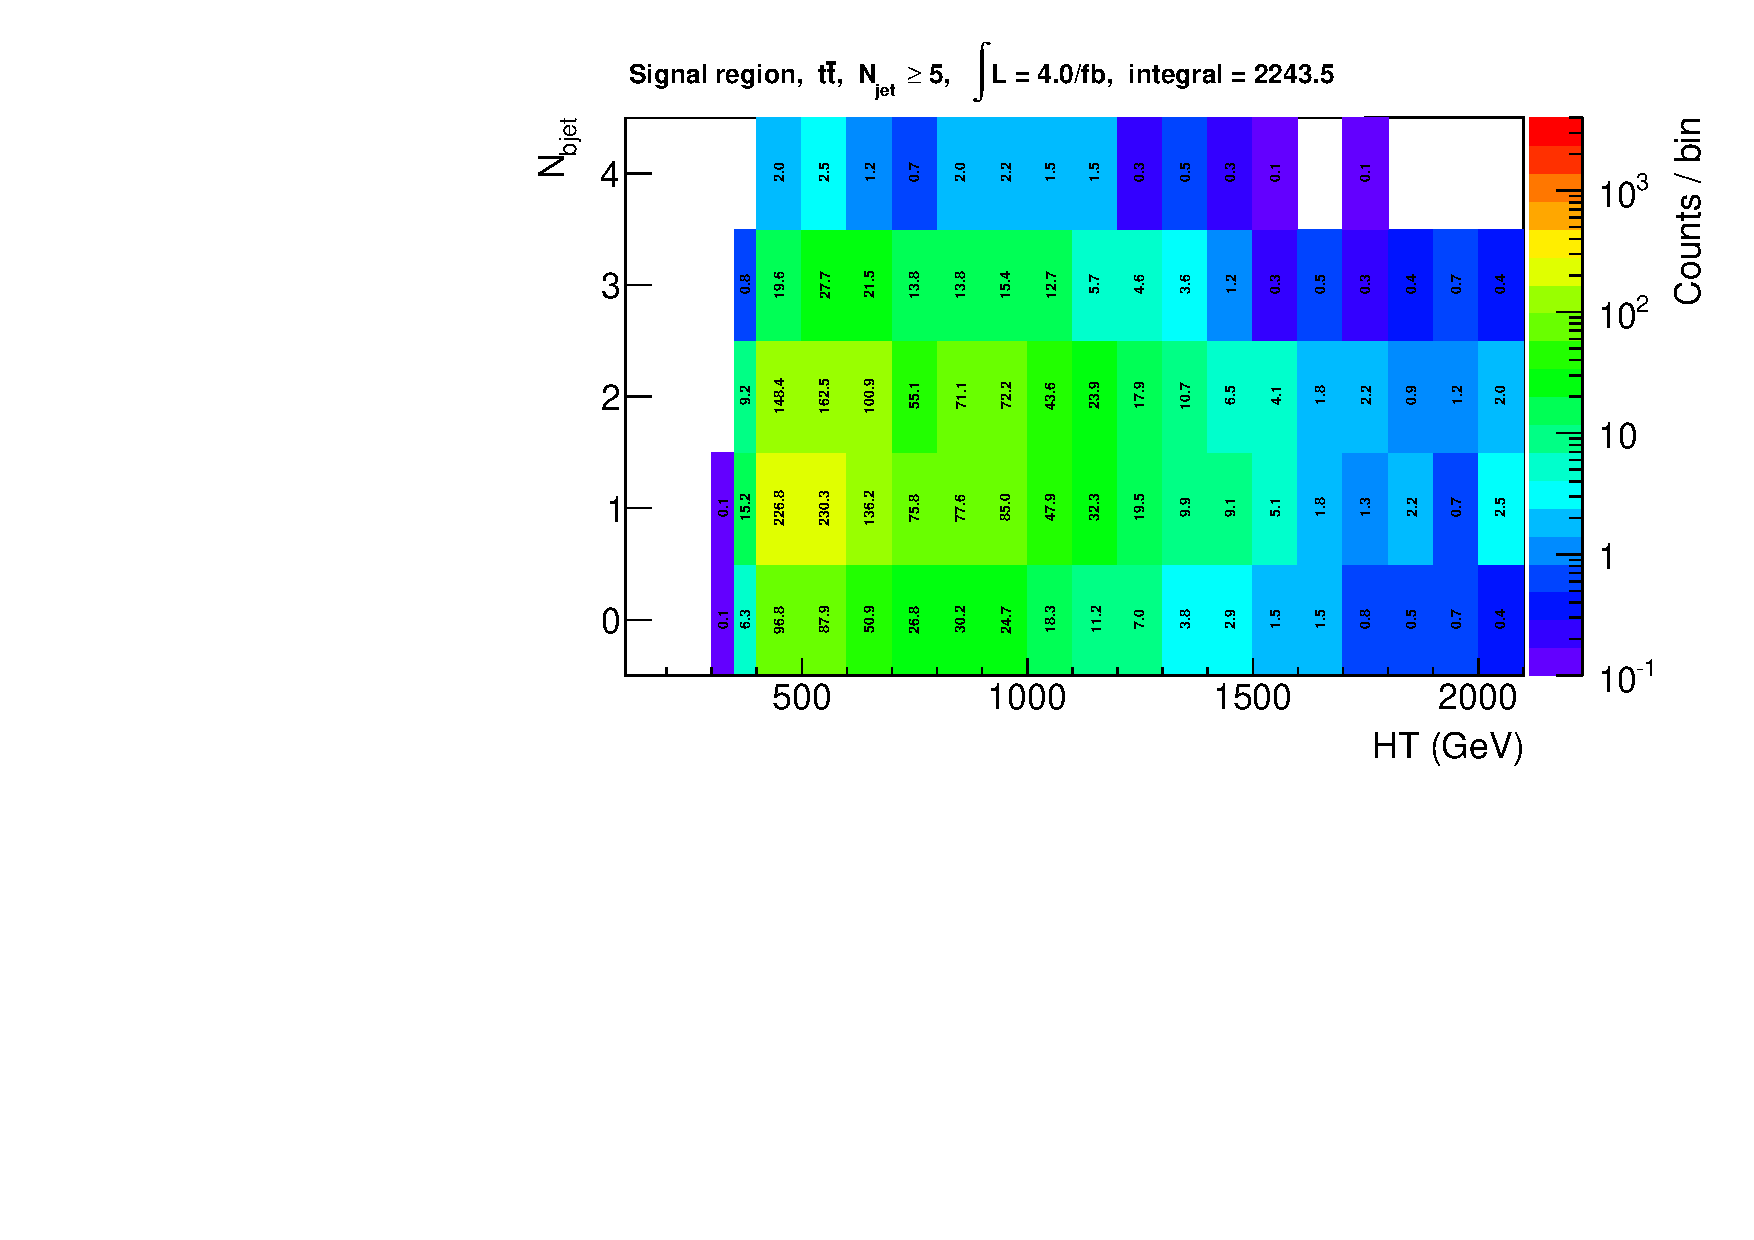
\includegraphics[width=0.5\textwidth]{figures/yieldPlots/had_ttbar_ge5j.pdf}
  }

  \\
  \subfigure[Hadronic signal region yields for T1bbbb simplified model
  \label{fig:sigYields}
  ($\njet \geq 5$)]{
    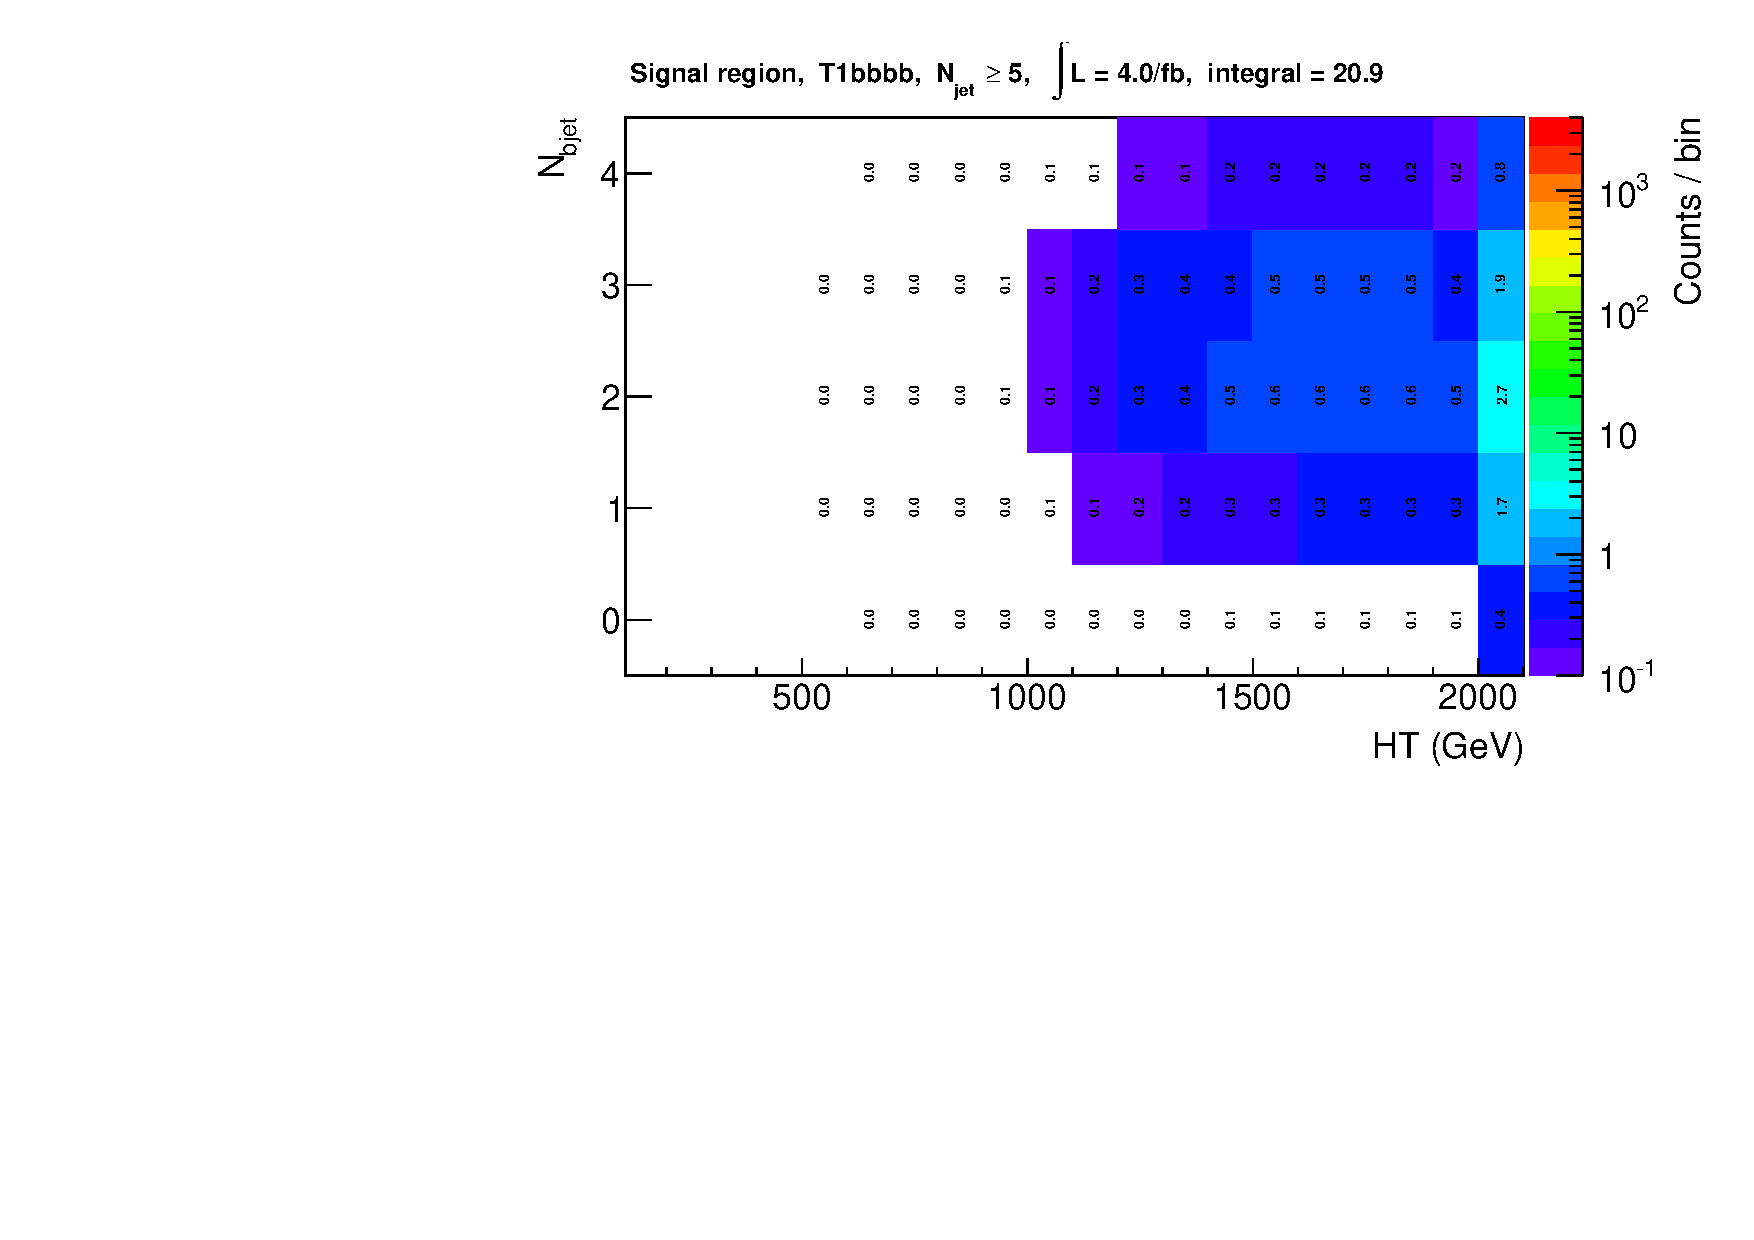
\includegraphics[width=0.5\textwidth]{figures/yieldPlots/sig_T1bbbb_ge5j.pdf}
  }
  \\
  \caption{\label{fig:ewkYields4} Yields at $4\fbinv$ for the electroweak backgrounds in the
  hadronic signal region, $\njet\geq5$. The binning is chosen to be in line with the analysis
  bins. The contribution from the dominant backgrounds is shown separately.}
\end{figure}

%%____________________________________________________________________________||
\subsection{Yields in the control samples}

The yields in the \mj, \mmj and \gj control samples can be seen in
Figures~\ref{fig:muYields}, \ref{fig:mumuYields} and \ref{fig:gammaYields}
respectively. The number of events in each of these bins is important for
working out how far we can extend in our analysis bins. We require there to be
enough events in the control samples to allow robust data driven prediction of
the backgrounds.

\begin{figure}[h!]
  \centering
  \subfigure[Yields from \texorpdfstring{\mj}{muon plus jets} control sample
  ($\njet = 2$)]{
    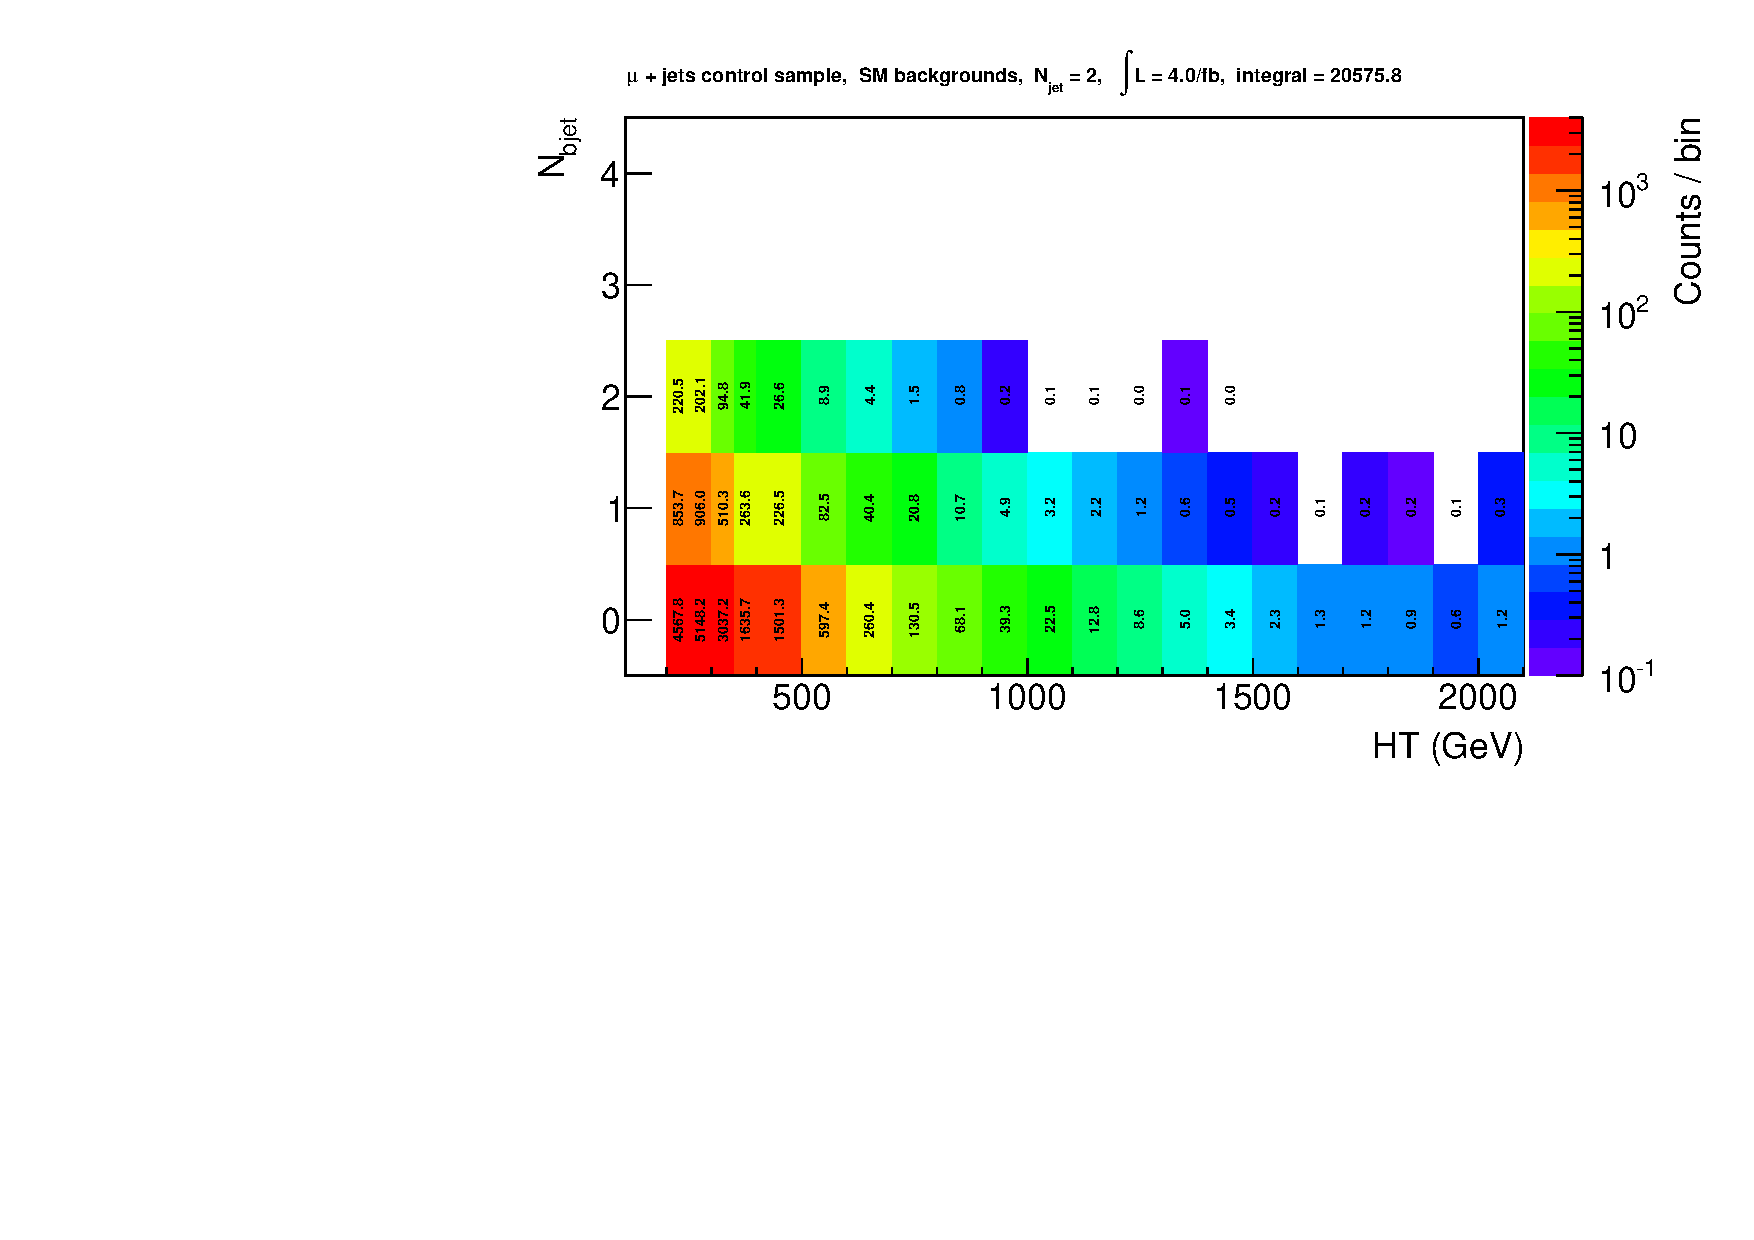
\includegraphics[width=0.5\textwidth]{figures/yieldPlots/mu_ewk_eq2j.pdf}
  }~~
  \subfigure[Yields from \texorpdfstring{\mj}{muon plus jets} control sample
  ($\njet = 3$)]{
    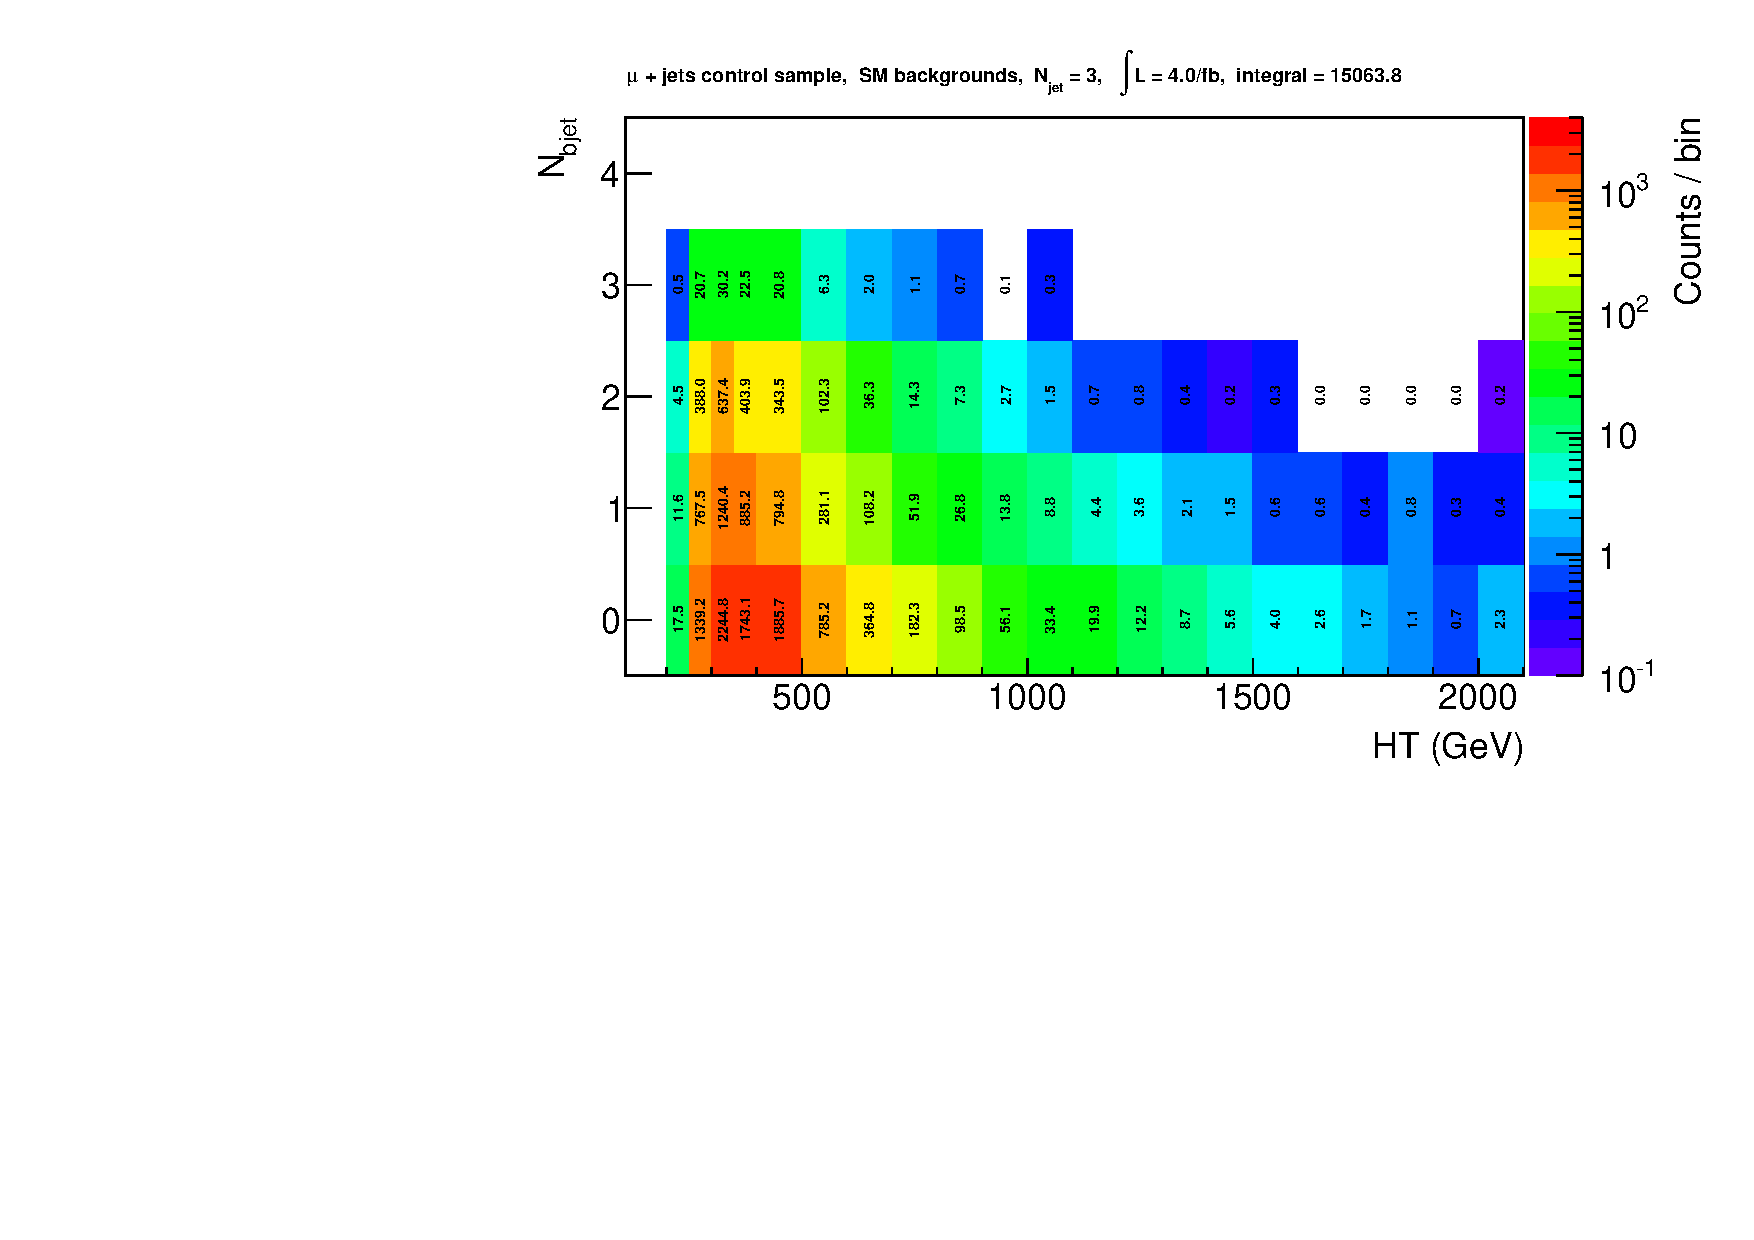
\includegraphics[width=0.5\textwidth]{figures/yieldPlots/mu_ewk_eq3j.pdf}
  }
  \\
  \subfigure[Yields from \texorpdfstring{\mj}{muon plus jets} control sample
  ($\njet = 4$)]{
    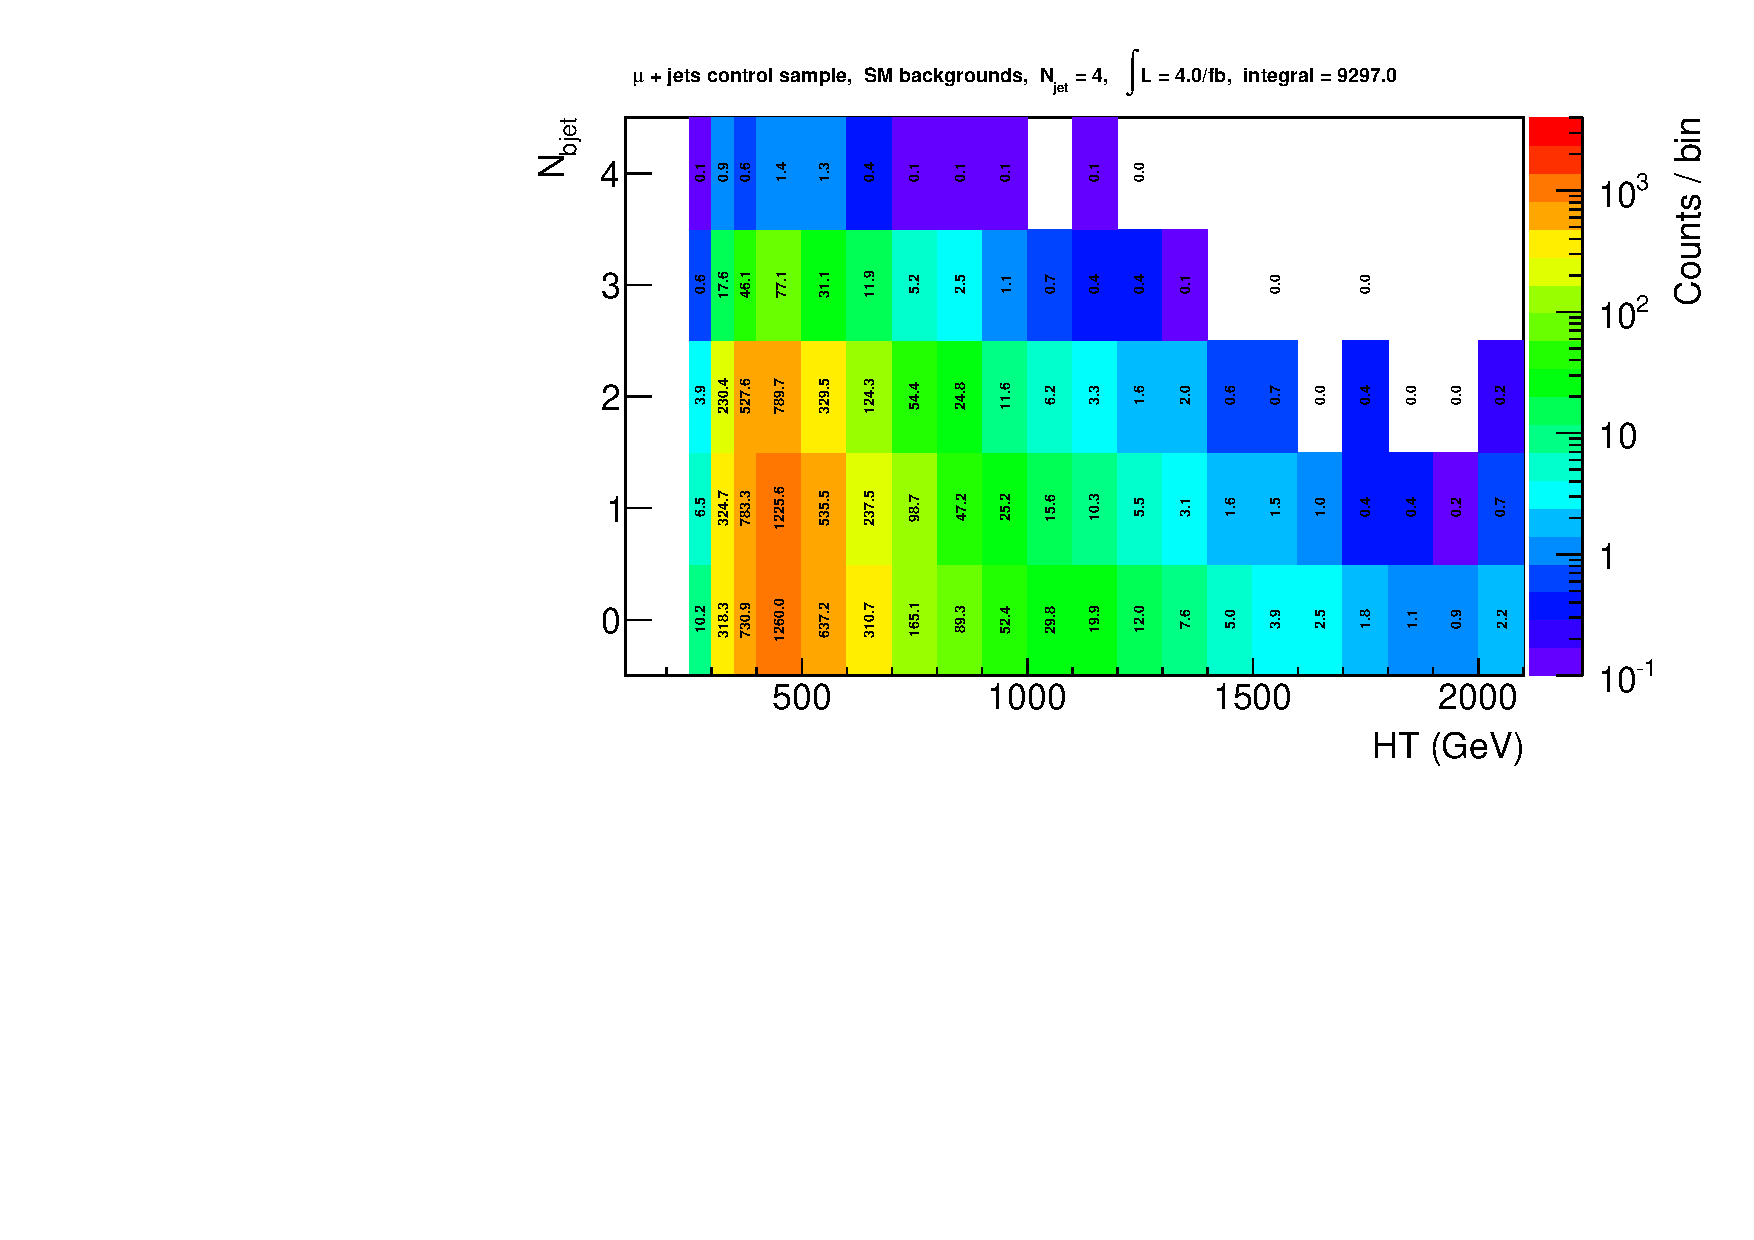
\includegraphics[width=0.5\textwidth]{figures/yieldPlots/mu_ewk_eq4j.pdf}
  }~~
  \subfigure[Yields from \texorpdfstring{\mj}{muon plus jets} control sample
  ($\njet \geq 5$)]{
    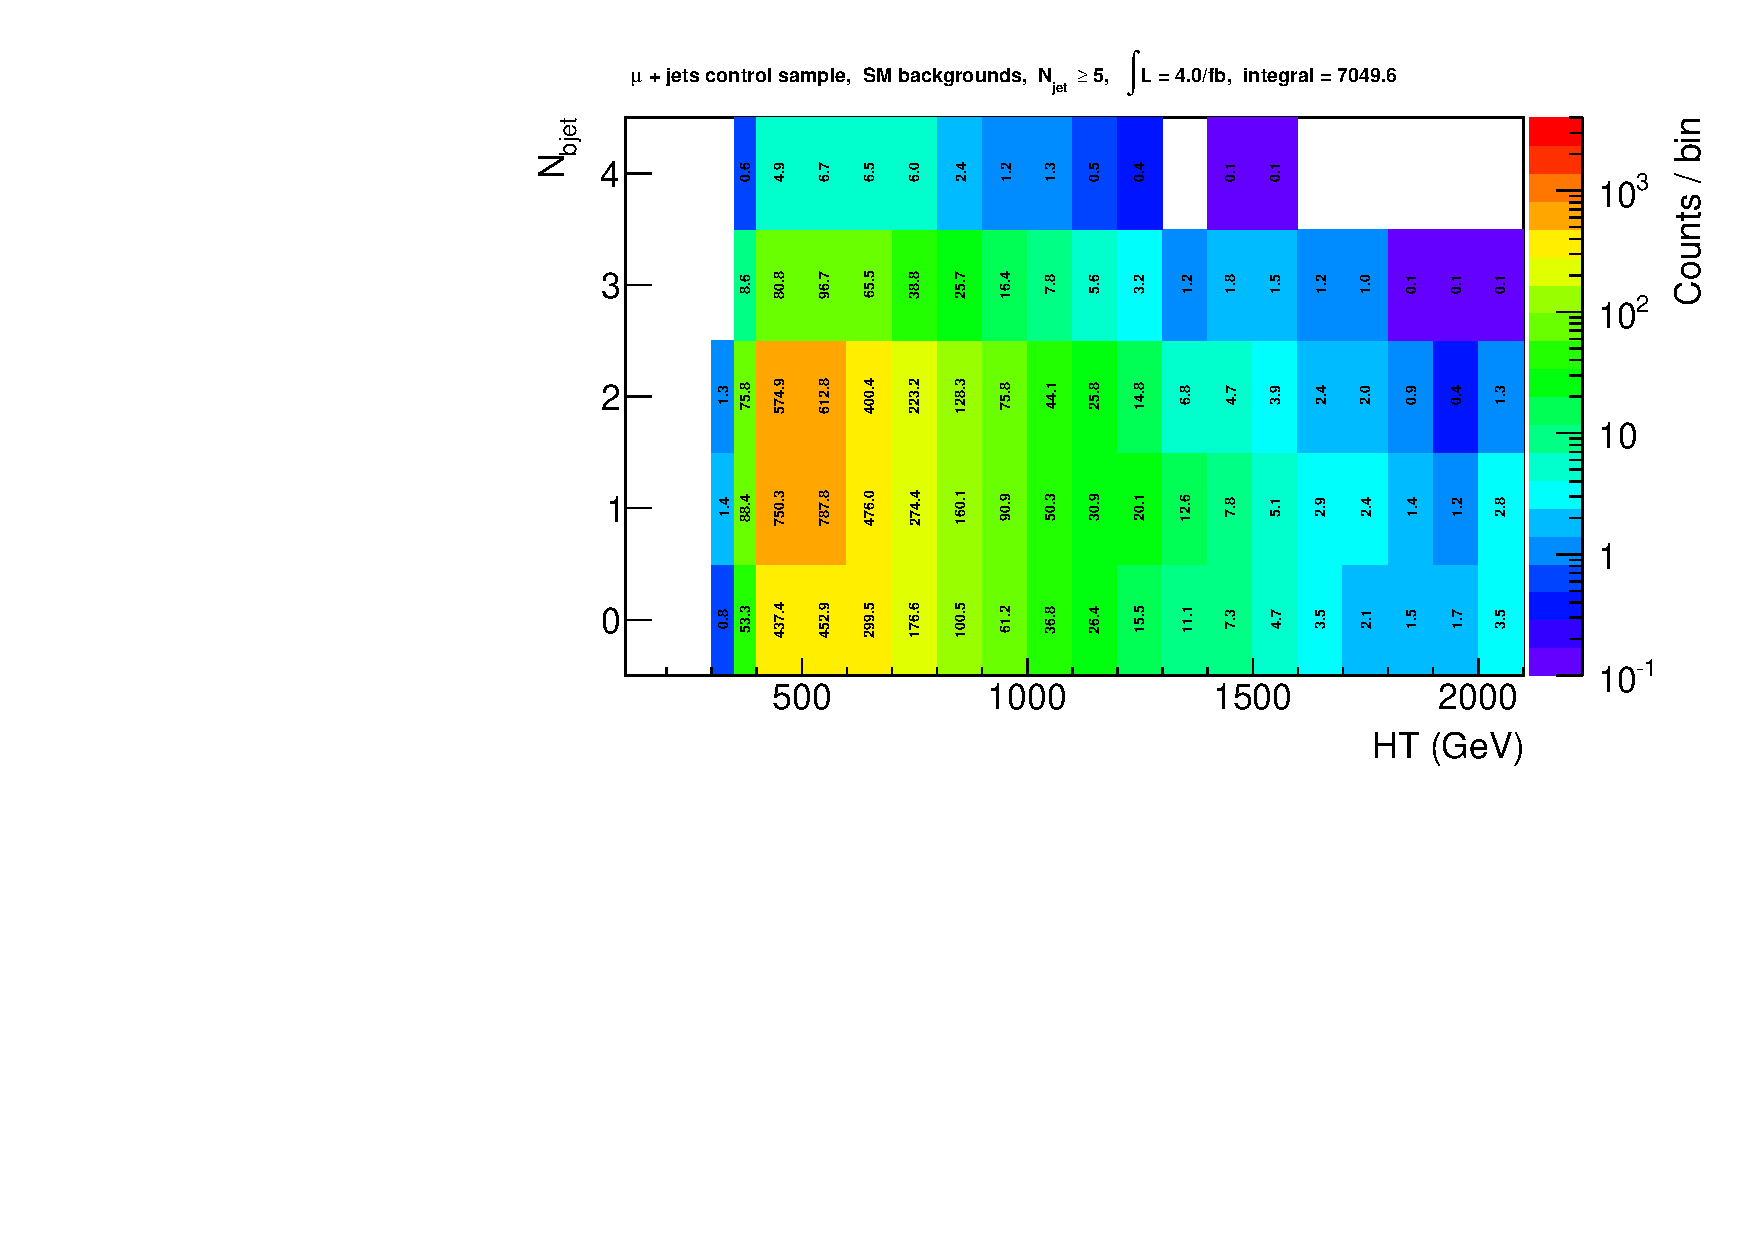
\includegraphics[width=0.5\textwidth]{figures/yieldPlots/mu_ewk_ge5j.pdf}
  } 
  \\
  \caption{\label{fig:muYields} Yields at $4\fbinv$ for the W~+~jets and \ttbar
  MC contributions to the \texorpdfstring{\mj}{muon plus jets} control sample. }
\end{figure}

\begin{figure}[h!]
  \centering
  \subfigure[Yields from \texorpdfstring{\mmj}{di-muon plus jets} control sample
  ($\njet = 2$)]{
    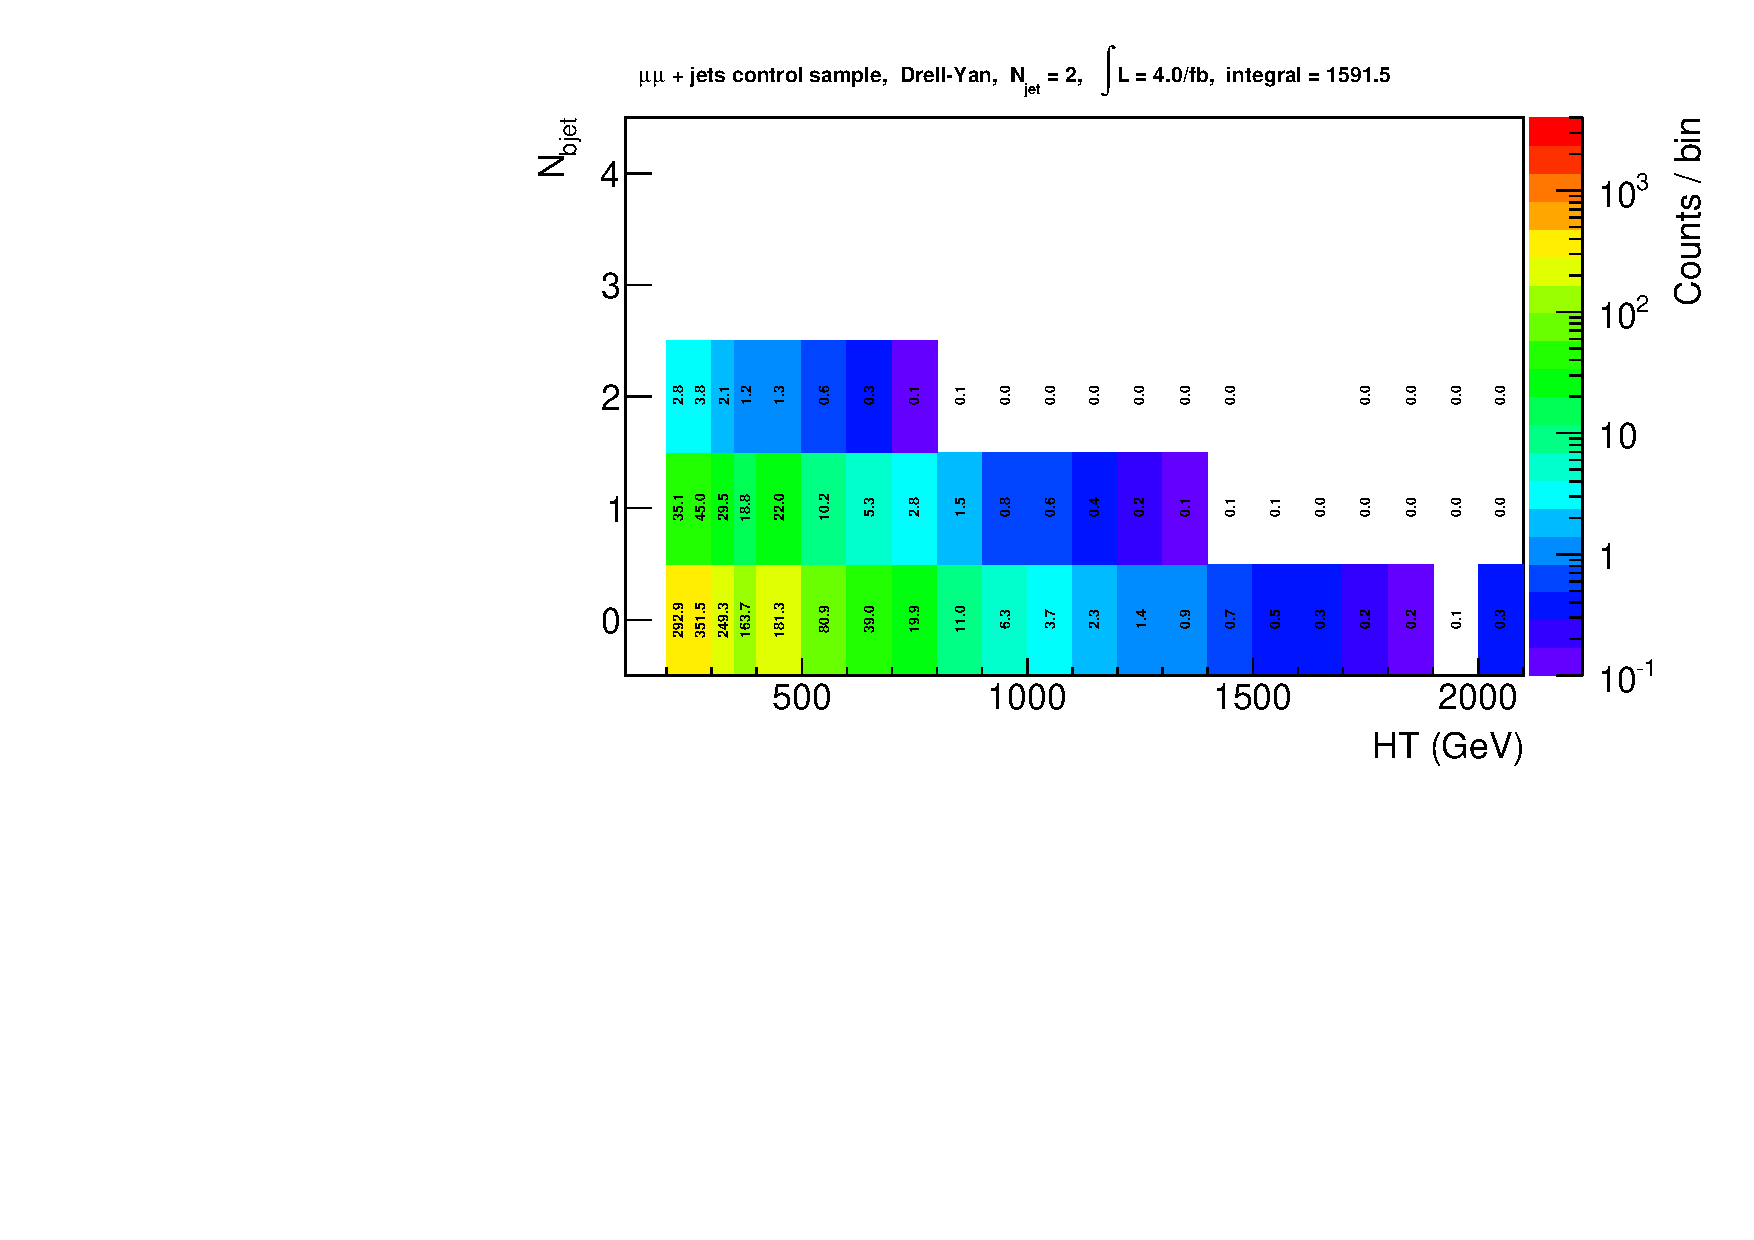
\includegraphics[width=0.5\textwidth]{figures/yieldPlots/mm_dy_eq2j.pdf}
  }~~
  \subfigure[Yields from \texorpdfstring{\mmj}{di-muon plus jets} control sample
  ($\njet = 3$)]{
    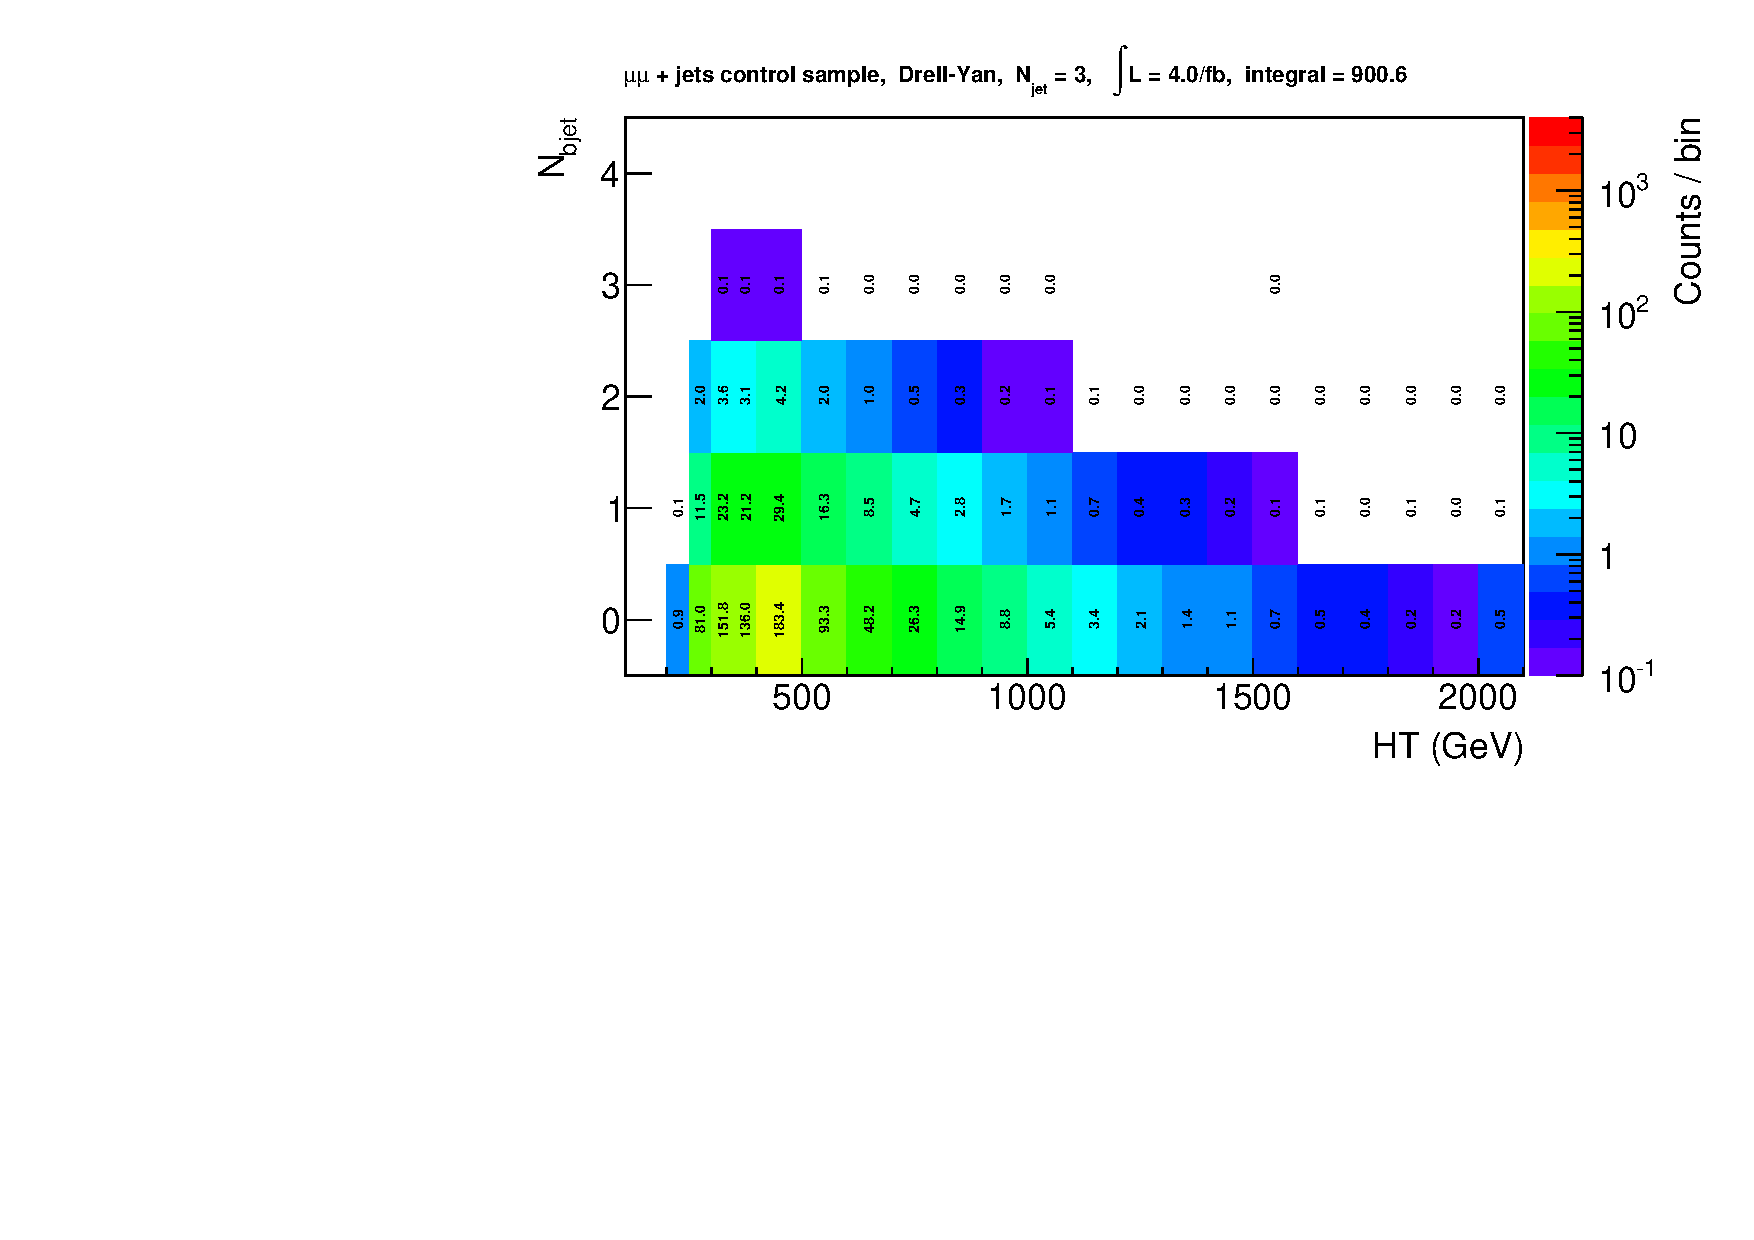
\includegraphics[width=0.5\textwidth]{figures/yieldPlots/mm_dy_eq3j.pdf}
  }
  \\
  \subfigure[Yields from \texorpdfstring{\mmj}{di-muon plus jets} control sample
  ($\njet = 4$)]{
    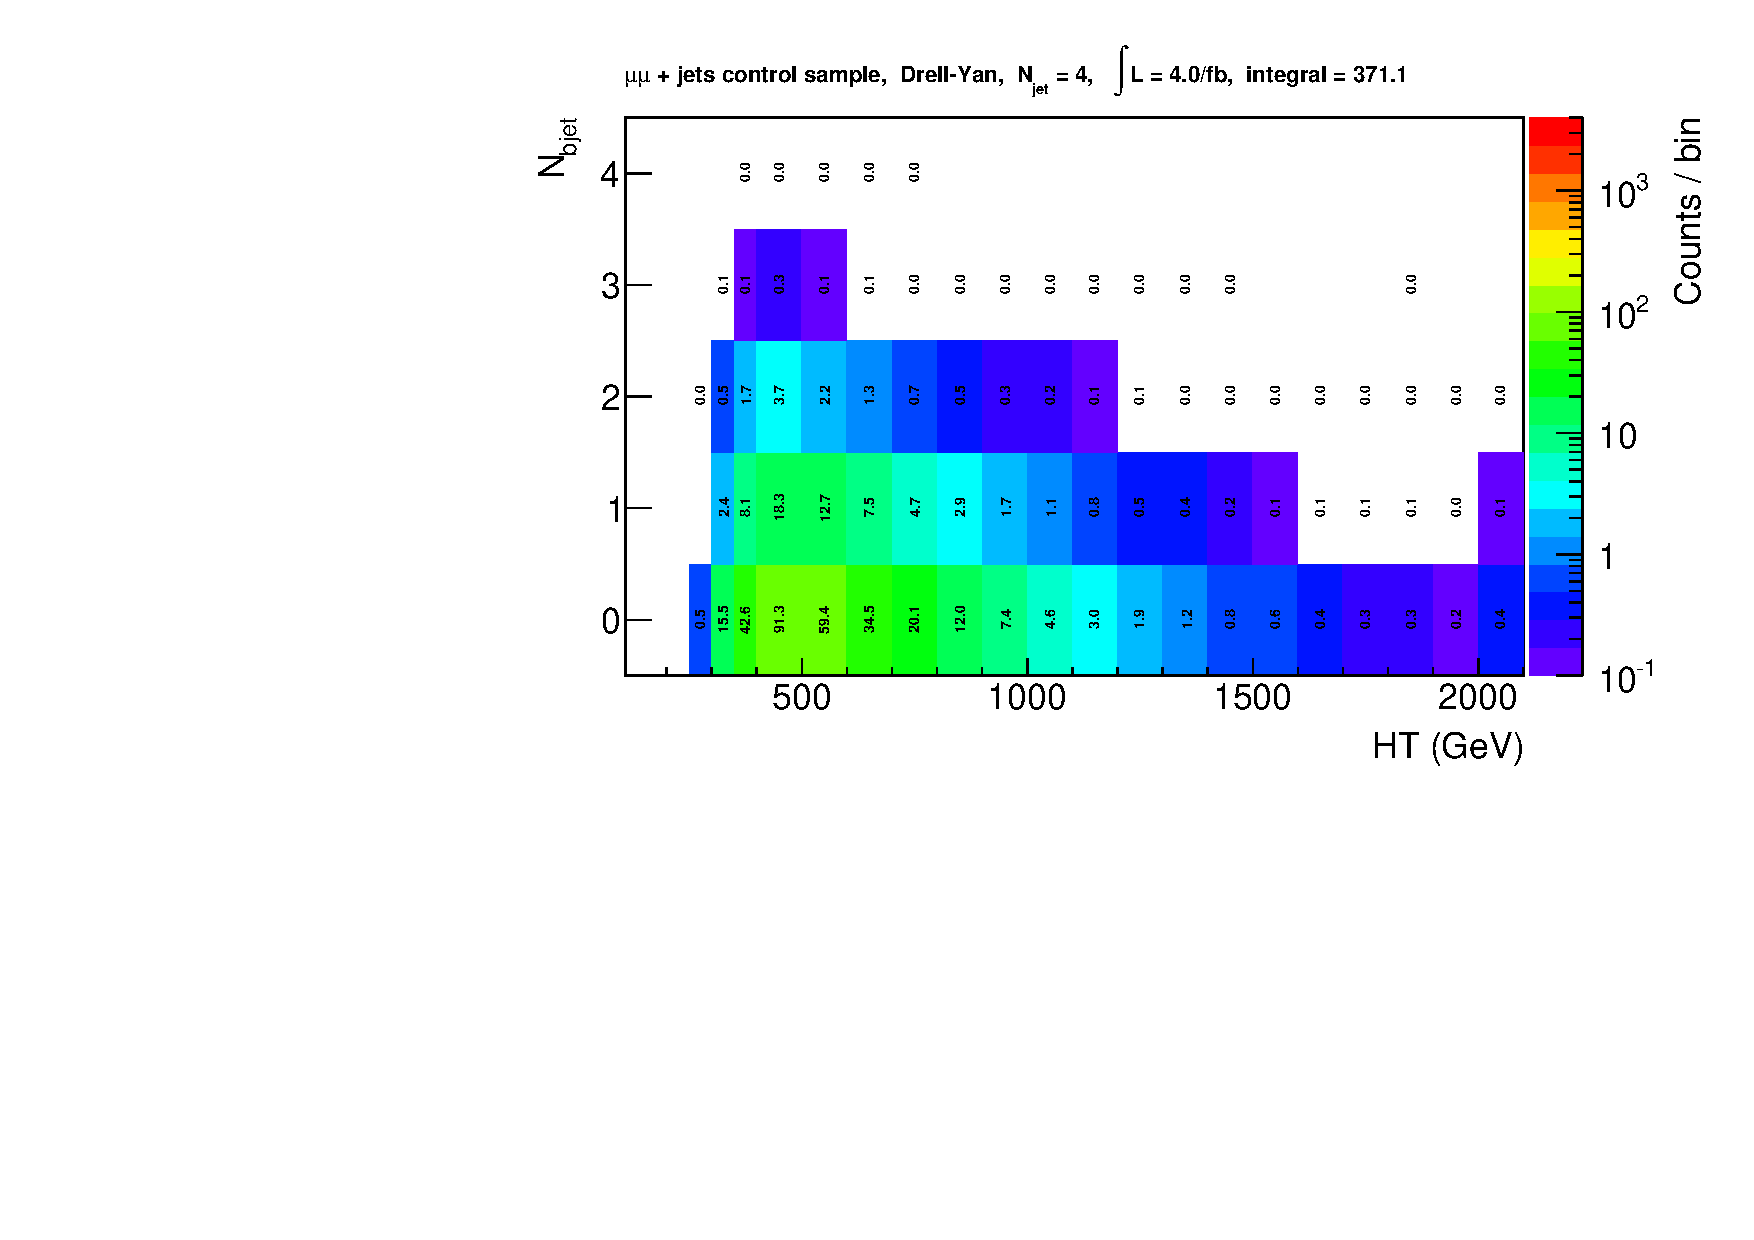
\includegraphics[width=0.5\textwidth]{figures/yieldPlots/mm_dy_eq4j.pdf}
  }~~
  \subfigure[Yields from \texorpdfstring{\mmj}{di-muon plus jets} control sample
  ($\njet \geq 5$)]{
    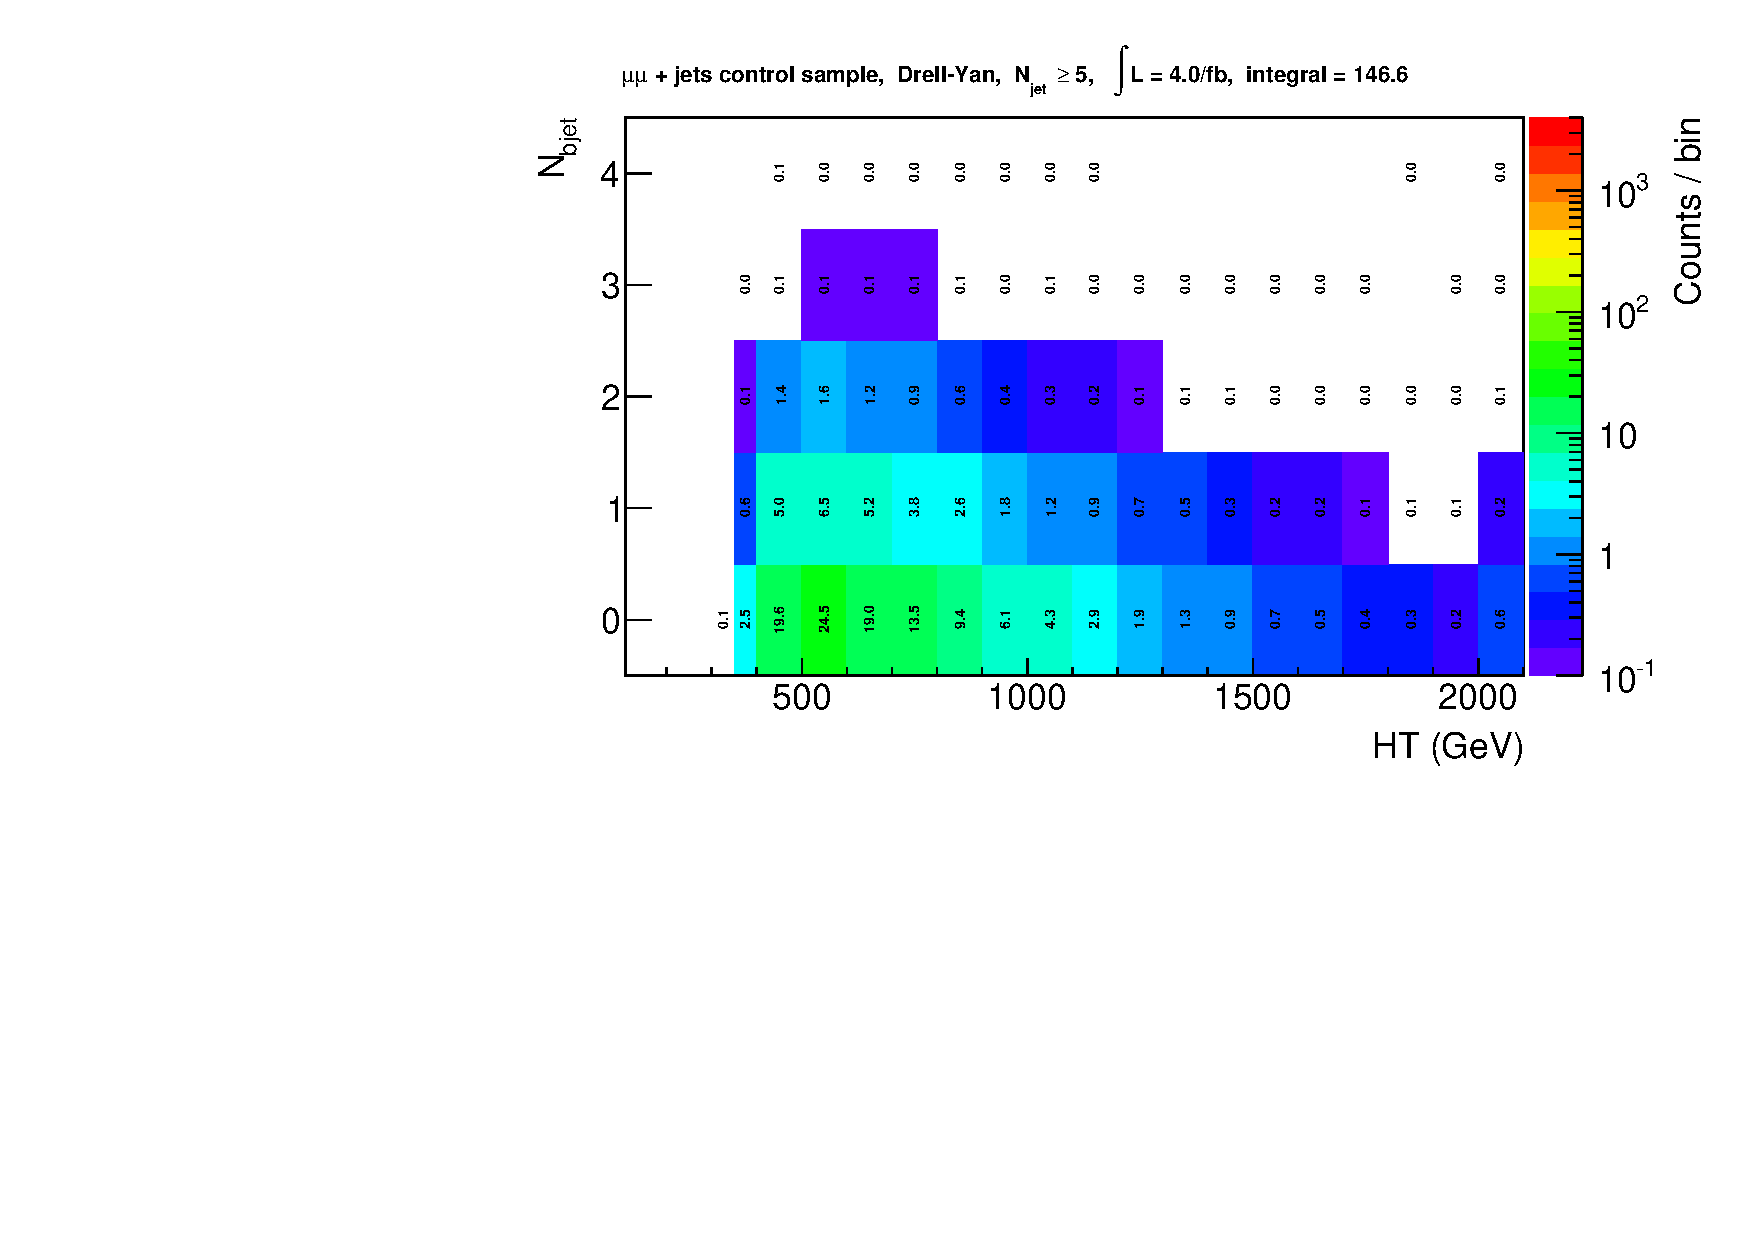
\includegraphics[width=0.5\textwidth]{figures/yieldPlots/mm_dy_ge5j.pdf}
  } 
  \\
  \caption{\label{fig:mumuYields} Yields at $4\fbinv$ for the DY~+~jets MC 
  contributions to the \texorpdfstring{\mmj}{di-muon plus jets} control sample. }
\end{figure}

\begin{figure}[h!]
  \centering
  \subfigure[Yields from \texorpdfstring{\gj}{photon plus jets} control sample
  ($\njet = 2$)]{
    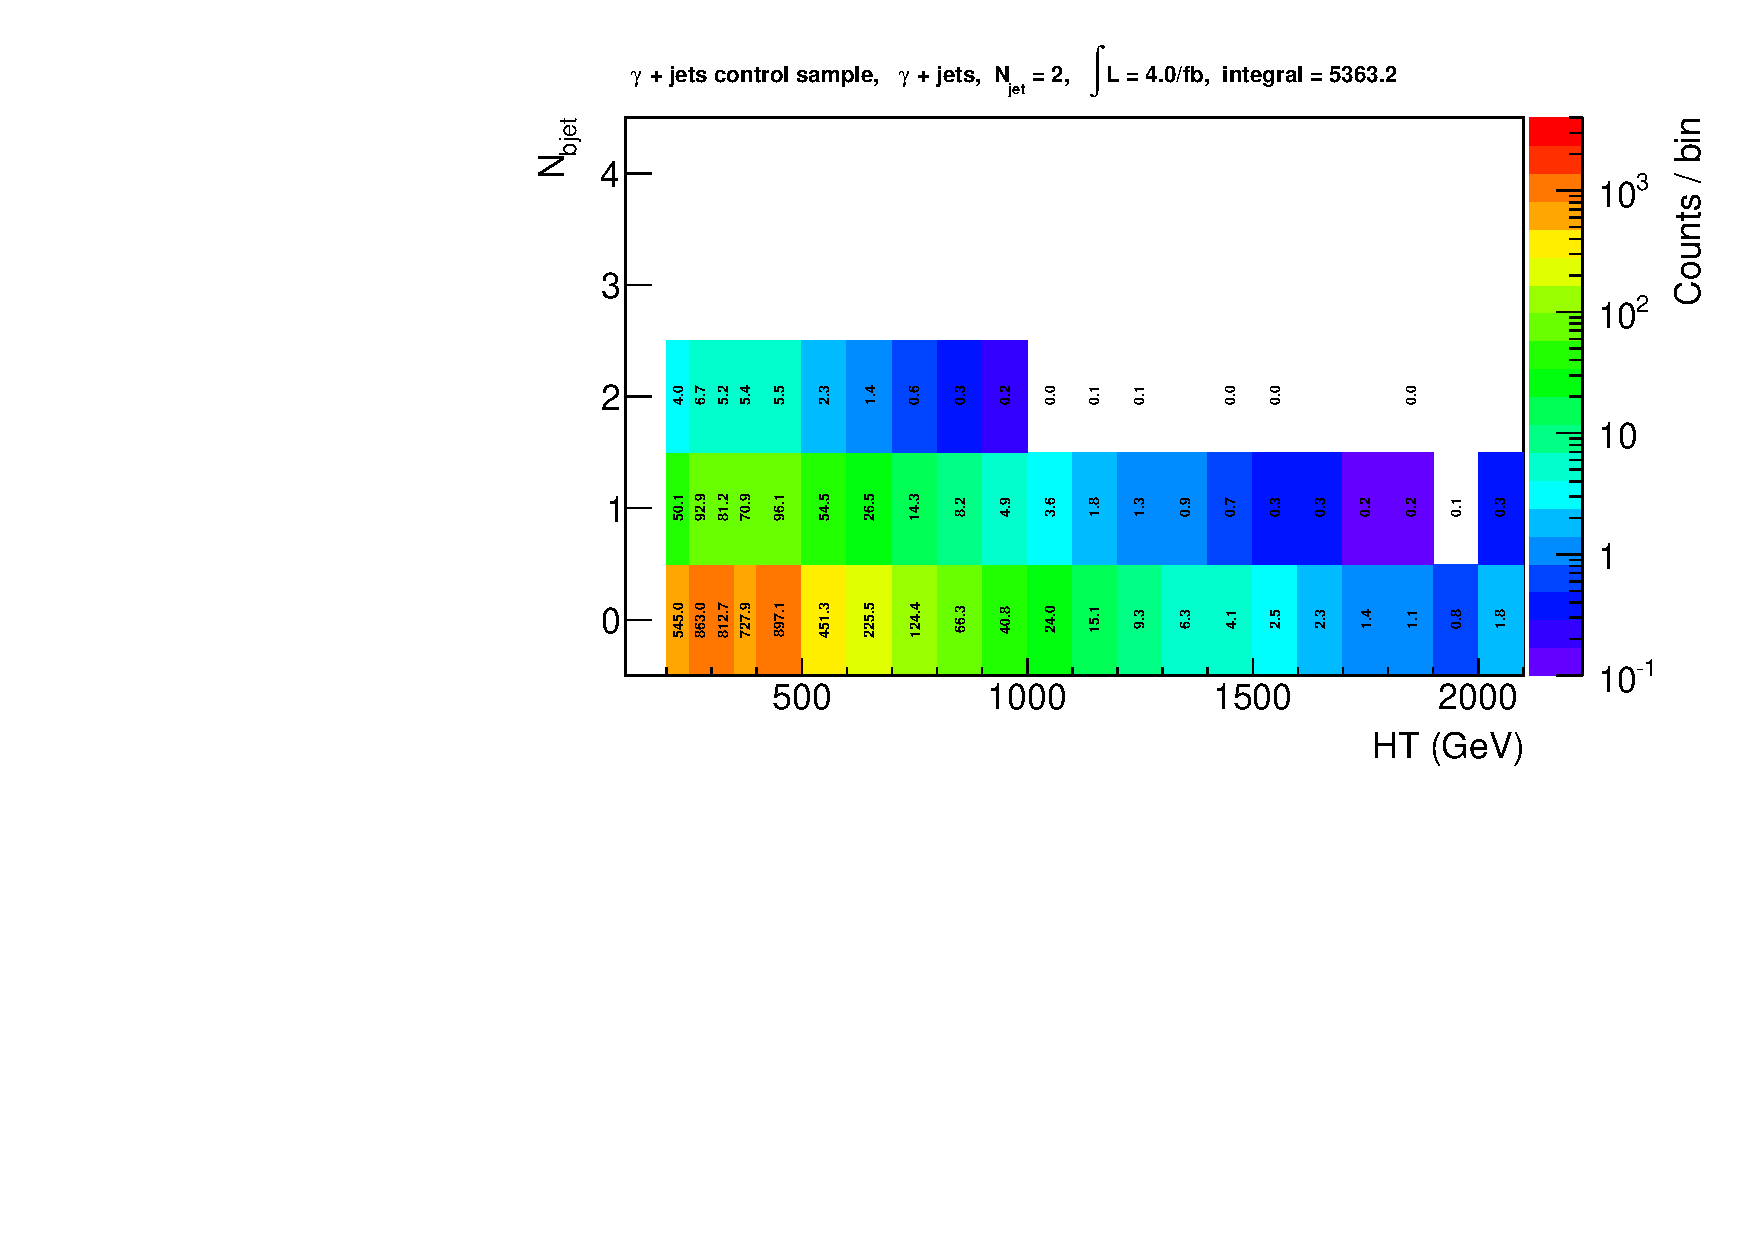
\includegraphics[width=0.5\textwidth]{figures/yieldPlots/ph_gjets_eq2j.pdf}
  }~~
  \subfigure[Yields from \texorpdfstring{\gj}{photon plus jets} control sample
  ($\njet = 3$)]{
    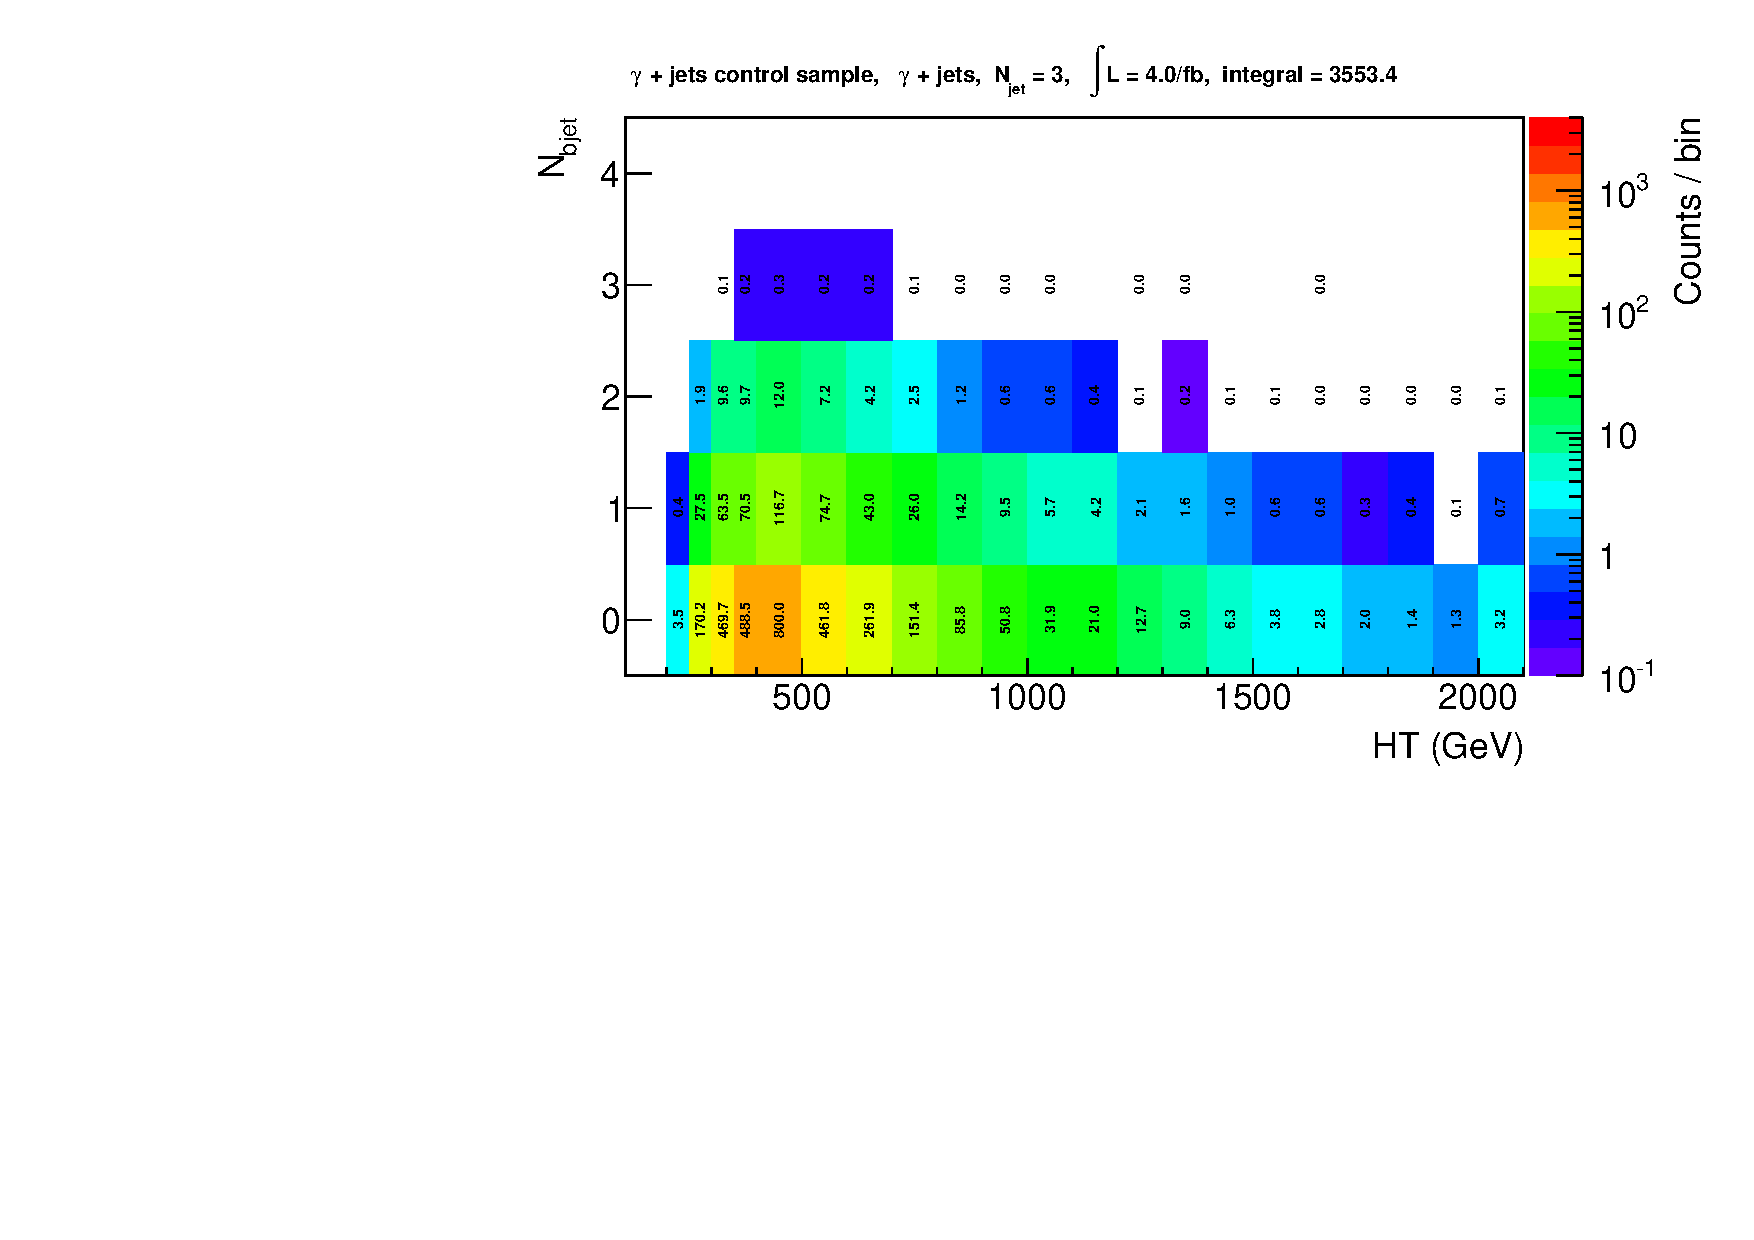
\includegraphics[width=0.5\textwidth]{figures/yieldPlots/ph_gjets_eq3j.pdf}
  }
  \\
  \subfigure[Yields from \texorpdfstring{\gj}{photon plus jets} control sample
  ($\njet = 4$)]{
    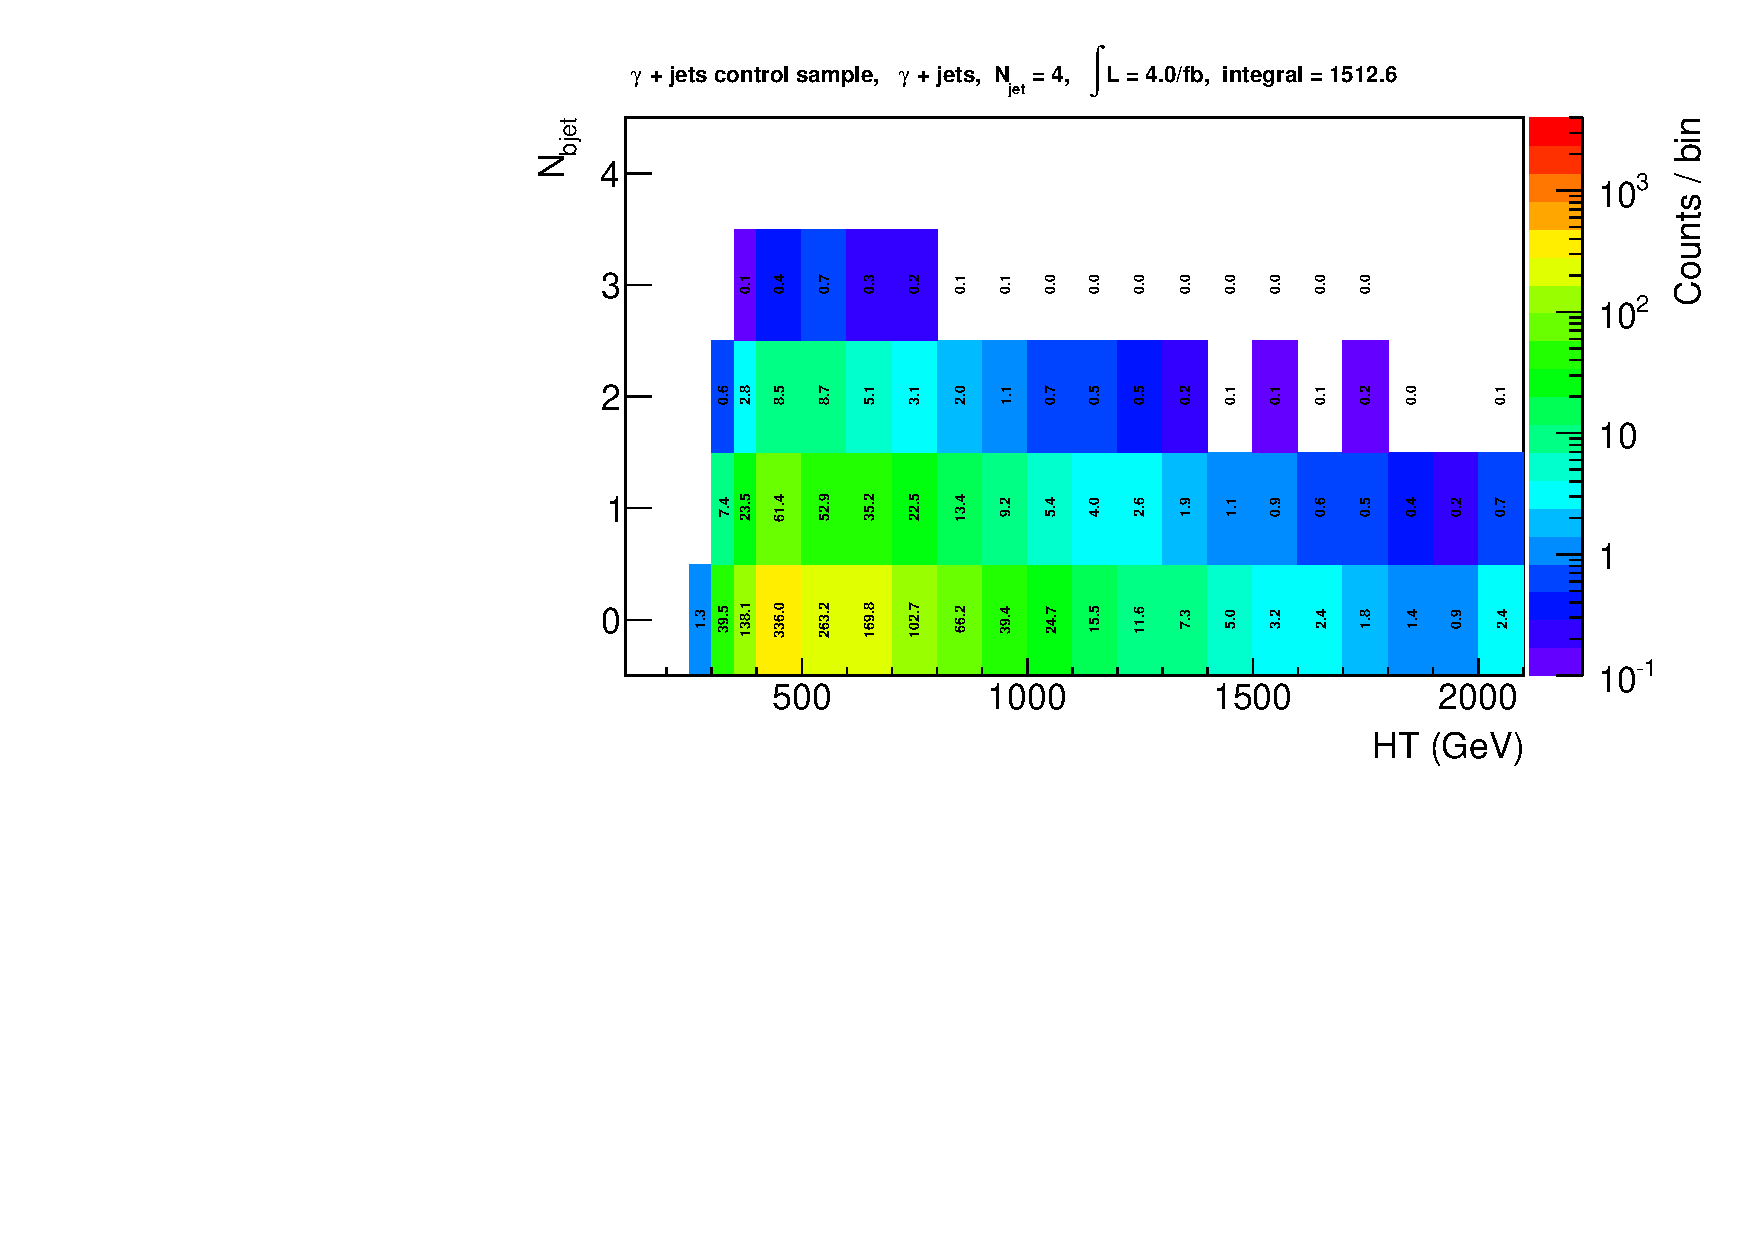
\includegraphics[width=0.5\textwidth]{figures/yieldPlots/ph_gjets_eq4j.pdf}
  }~~
  \subfigure[Yields from \texorpdfstring{\gj}{photon plus jets} control sample
  ($\njet \geq 5$)]{
    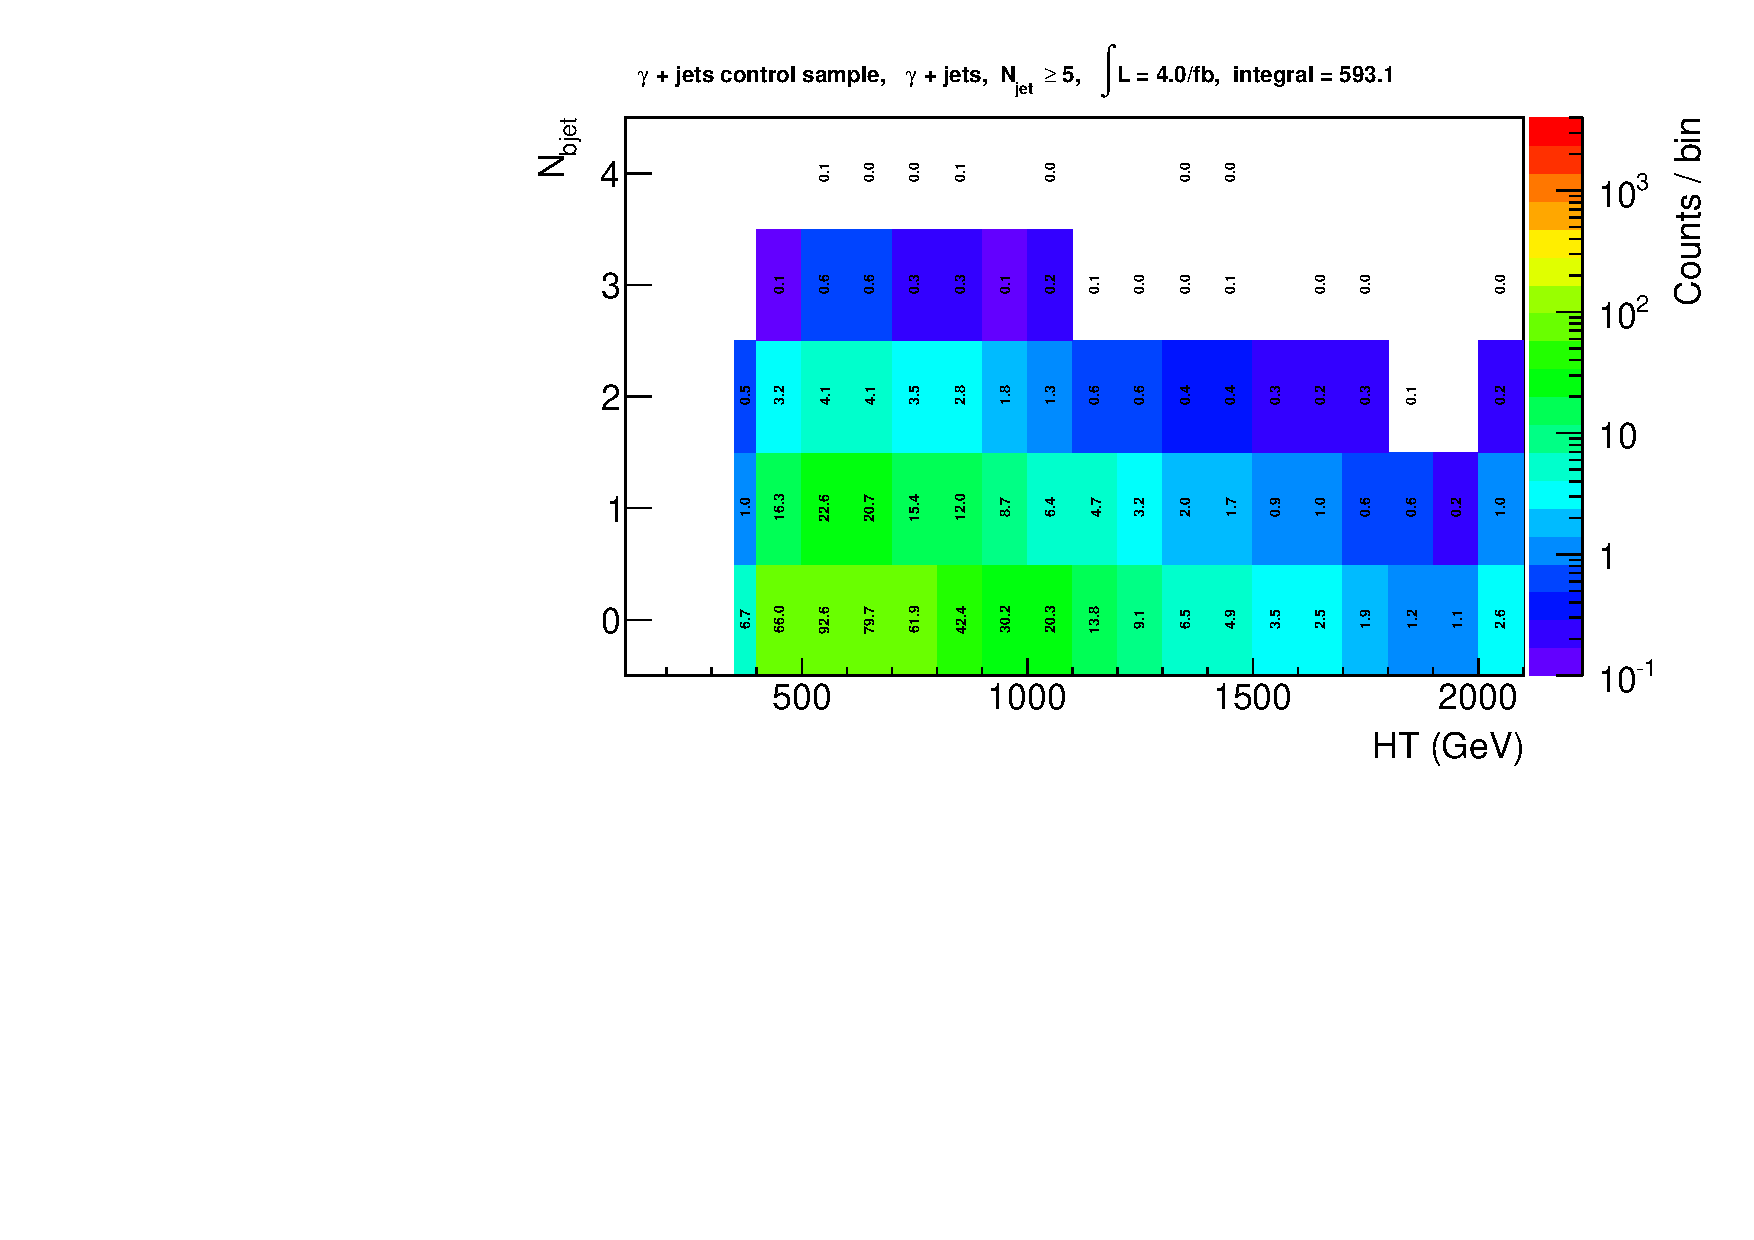
\includegraphics[width=0.5\textwidth]{figures/yieldPlots/ph_gjets_ge5j.pdf}
  } 
  \\
  \caption{\label{fig:gammaYields} Yields at $4\fbinv$ for the GJets MC 
  contributions to the \texorpdfstring{\gj}{photon plus jets} control sample. }
\end{figure}

%%____________________________________________________________________________||
\subsection{The improvement of sensitivity to SUSY and DM models with binning changes}

\subsubsection{Signal }\label{sec:asym_bin}

For a typical compressed model, Fig.~\ref{fig:asymMotivation} shows the second jet \PT
distribution for two different \HT bins. In the low \HT case a large portion of
the events are killed by requiring the second jet to have $\ET>100\gev$. 

We therefore add an new analysis category where the leading jet is required to fulfill 
momenta of jet $\ET>100\gev$ and sub-leading jet $40\gev<\ET<100\gev$. This new category 
results in new asymmetric jet bins split also in $\njet$, $\nb$ and \HT. The asymmetric jet bin
results in much larger acceptance for monojet-type and ISR induced event topologies like DM signals
and compresses SUSY scenarios. 
For the simplified model T2tt with $m_{stop}=425\gev$ and $m_{LSP}=325\gev$, 
including these bins increases signal acceptance by around a factor 3, for the DM models a factor of five is observed.
The asymmetric bins will be added to the nominal selection, thus in combination the for all models the analysis power can only improve or remain constant.
\begin{figure}[h!]
  \centering
  \subfigure[Second jet \PT for $200\gev<\HT<250\gev$, $\alphat>0.65$]{
    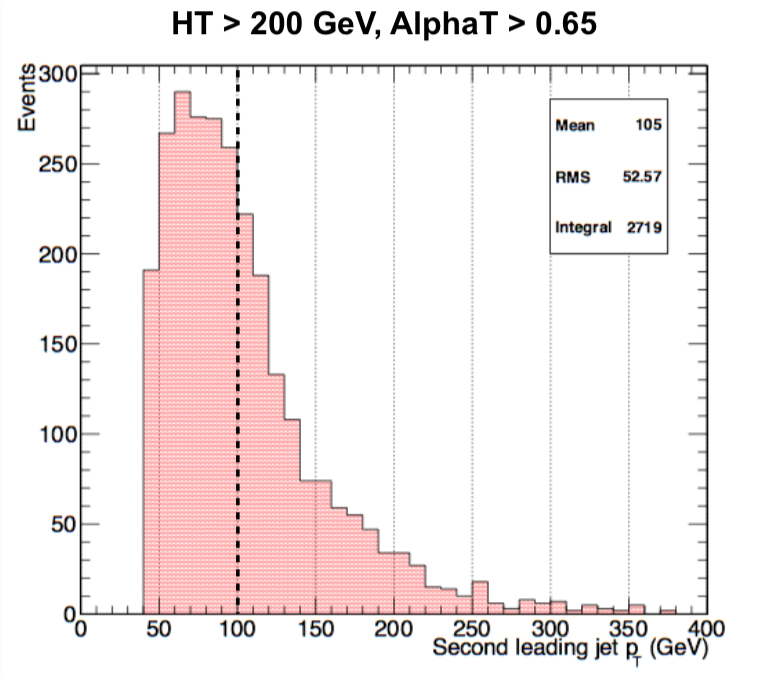
\includegraphics[width=0.5\textwidth]{figures/asymPlots/secondJetPtlowHT}
  }~~
  \subfigure[Second jet \PT for $400\gev<\HT>500\gev$, $\alphat>0.52$]{
    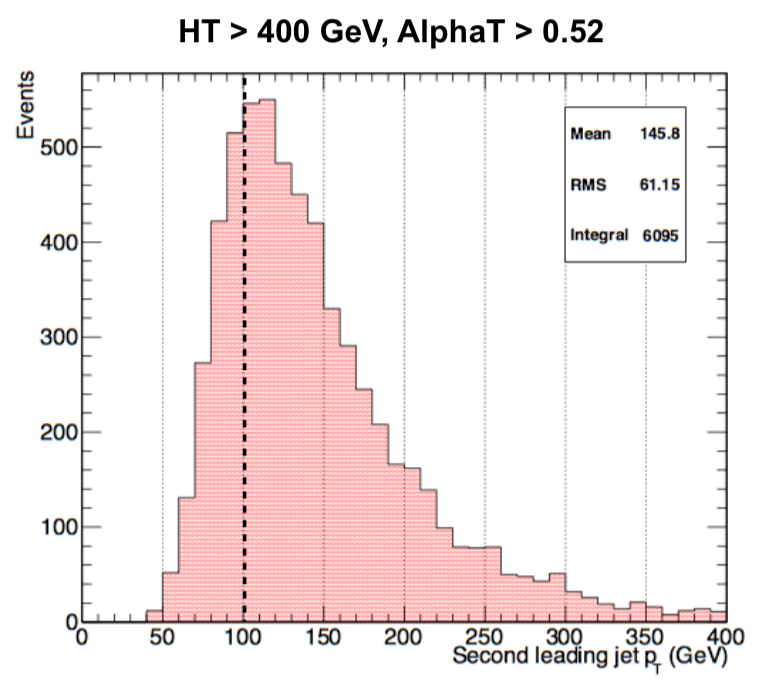
\includegraphics[width=0.5\textwidth]{figures/asymPlots/secondJetPthigherHT}
  }
  \\
  \caption{\label{fig:asymMotivation} The second leading jet \PT for different
  cases of \HT after a baseline signal selection: $\njet\geq2$, lead jet
  $\ET>100\gev$, lepton vetoes. Made with the T2tt ($m_{STOP}=425\gev$, $m_{LSP}=325\gev$) simplified model sample.}
\end{figure}

\subsubsection{Extension of \HT bins}

The production of heavy SUSY particles, such as gluino pair
production, will result in large values of \HT . This is illustrated in the high 
\HT of events in Fig.~\ref{fig:sigYields}. To increase the sensitivity
of the analysis to these kinds of models, the \HT bins can be extended to higher
values. The only limit placed on this value is that there are enough events in the
relevant control samples, to allow a data driven background prediction. The
number of events is deemed to be sufficient when their statistical uncertainty is
approximately equal to the expected systematic uncertainty for the bin in
question. Initial studies suggest it should be possible to extend up to
$\HT=1600$, possibly even $\HT=2000$. This would give a great increase in the
signal over background ratio, particularly for gluino mediated models.

\clearpage
%%____________________________________________________________________________||
\subsection{Signal yields for the asymmetric selection}
The effect of the asymetric bins designed to increase acceptance for monojet-type and ISR induced final stats has been tested using the DM samples defined in Tab.~\ref{tab:datasets_dm}. Details regarding the asymetric jet categories are given in Sec.~\ref{sec:asym_bin}.
For illustration purposes we consider only the bins up to $H_\textrm{T}=700$~GeV and jet multiplicities up to $n_j=4$ in Tab.~\ref{tab:sig_yields_AVDM_nom}-\ref{tab:sig_yields_VDM_asym}.

\begin{table}[h]
\small
\begin{tabular}{lllllllll}
\hline \hline
$H_\textrm{T}$                 &     200 &            250 &             300&             350&             400&             500&             600&             700  \\\hline\hline
$2j 0b$&          16 (0.04)&	   25 (0.03)&	   24 (0.03)&	   19 (0.03)&	   24 (0.03)&	   14 (0.04)&	    7 (0.05)&	    5 (0.07) \\\hline
$2j 1b$&           1 (0.13)&	    2 (0.10)&	    2 (0.10)&	    2 (0.11)&	    3 (0.08)&	    2 (0.12)&	    1 (0.16)&	    1 (0.20) \\\hline
$2j 2b$&           0 (0.50)&	    0 (0.50)&	    0 (0.38)&	    0 (0.41)&	    0 (0.45)&	    0 (0.58)&	    0 (0.58)&	    0 (1.00) \\\hline
$3j 0b$&           0 ( nan)&	    5 (0.07)&	   14 (0.04)&	   18 (0.03)&	   31 (0.03)&	   20 (0.03)&	   13 (0.04)&	    8 (0.05) \\\hline
$3j 1b$&           0 ( nan)&	    0 (0.21)&	    2 (0.12)&	    2 (0.10)&	    4 (0.07)&	    3 (0.09)&	    2 (0.10)&	    1 (0.12) \\\hline
$3j 2b$&           0 ( nan)&	    0 (1.00)&	    0 (0.30)&	    0 (0.30)&	    1 (0.20)&	    0 (0.23)&	    0 (0.32)&	    0 (0.38) \\\hline
$3j 3b$&           0 ( nan)&	    0 ( nan)&	    0 ( nan)&	    0 ( nan)&	    0 ( nan)&	    0 ( nan)&	    0 (1.00)&	    0 (1.00) \\\hline
$4j 0b$&           0 ( nan)&	    0 (0.71)&	    1 (0.13)&	    6 (0.06)&	   15 (0.04)&	   15 (0.04)&	   10 (0.05)&	    7 (0.06) \\\hline
$4j 1b$&           0 ( nan)&	    0 ( nan)&	    0 (0.33)&	    1 (0.17)&	    3 (0.09)&	    2 (0.09)&	    2 (0.11)&	    2 (0.12) \\\hline
$4j 2b$&           0 ( nan)&	    0 ( nan)&	    0 (1.00)&	    0 (0.41)&	    0 (0.22)&	    0 (0.22)&	    0 (0.25)&	    0 (0.50) \\\hline
$4j 3b$&           0 ( nan)&	    0 ( nan)&	    0 ( nan)&	    0 ( nan)&	    0 ( nan)&	    0 ( nan)&	    0 (1.00)&	    0 ( nan) \\\hline
$4j 4b$&           0 ( nan)&	    0 ( nan)&	    0 ( nan)&	    0 ( nan)&	    0 ( nan)&	    0 ( nan)&	    0 ( nan)&	    0 ( nan) \\\hline
\hline
\end{tabular}
\caption{Signal yields for $H_\textrm{T}$ up to 700~GeV and up to 4 jets in the nominal selection for the axial-vector DM sample.}
\label{tab:sig_yields_AVDM_nom}
\end{table}

\begin{table}[h]
\begin{tabular}{lllllllll}
\hline \hline
$H_\textrm{T}$                 &     200 &            250 &             300&             350&             400&             500&             600&             700  \\\hline\hline
Asym. $2j 0b$&     66 (0.02)&	   34 (0.02)&	   20 (0.03)&	   12 (0.04)&	   13 (0.04)&	    6 (0.06)&	    2 (0.09)&	    1 (0.14) \\\hline
Asym. $2j 1b$&      5 (0.06)&	    3 (0.08)&	    2 (0.11)&	    1 (0.12)&	    1 (0.13)&	    1 (0.18)&	    0 (0.35)&	    0 (0.45) \\\hline
Asym. $2j 2b$&      0 (0.27)&	    0 (0.33)&	    0 (0.45)&	    0 (0.50)&	    0 (0.41)&	    0 (1.00)&	    0 ( nan)&	    0 (1.00) \\\hline
Asym. $3j 0b$&     15 (0.04)&	   24 (0.03)&	   18 (0.03)&	   10 (0.05)&	    9 (0.05)&	    3 (0.08)&	    1 (0.13)&	    0 (0.24) \\\hline
Asym. $3j 1b$&      2 (0.12)&	    3 (0.09)&	    2 (0.10)&	    1 (0.12)&	    1 (0.14)&	    0 (0.23)&	    0 (0.32)&	    0 (0.50) \\\hline
Asym. $3j 2b$&      0 (0.26)&	    0 (0.25)&	    0 (0.27)&	    0 (0.45)&	    0 (0.33)&	    0 (0.58)&	    0 (1.00)&	    0 ( nan) \\\hline
Asym. $3j 3b$&      0 (1.00)&	    0 ( nan)&	    0 (1.00)&	    0 (1.00)&	    0 ( nan)&	    0 ( nan)&	    0 ( nan)&	    0 ( nan) \\\hline
Asym. $4j 0b$&      0 (0.58)&	    3 (0.09)&	    7 (0.06)&	    6 (0.06)&	    5 (0.06)&	    2 (0.11)&	    1 (0.19)&	    0 (0.27) \\\hline
Asym. $4j 1b$&      0 (1.00)&	    0 (0.28)&	    1 (0.14)&	    1 (0.15)&	    1 (0.17)&	    0 (0.23)&	    0 (0.33)&	    0 (0.58) \\\hline
Asym. $4j 2b$&      0 ( nan)&	    0 (0.50)&	    0 (0.30)&	    0 (0.41)&	    0 (0.58)&	    0 (0.71)&	    0 (0.71)&	    0 ( nan) \\\hline
Asym. $4j 3b$&      0 ( nan)&	    0 (1.00)&	    0 ( nan)&	    0 ( nan)&	    0 ( nan)&	    0 ( nan)&	    0 ( nan)&	    0 ( nan) \\\hline
Asym. $4j 4b$&      0 ( nan)&	    0 ( nan)&	    0 ( nan)&	    0 ( nan)&	    0 ( nan)&	    0 ( nan)&	    0 ( nan)&	    0 ( nan) \\\hline
\hline              
\end{tabular}
\caption{Signal yields for $H_\textrm{T}$ up to 700~GeV and up to 4 jets in the asymmetric jet selection for the axial-vector DM sample.}
\label{tab:sig_yields_AVDM_asym}
\end{table}





\begin{table}[h]
\small
\begin{tabular}{lllllllll}
\hline \hline
$H_\textrm{T}$                 &     200 &            250 &             300&             350&             400&             500&             600&             700  \\\hline\hline
$2j 0b$&          16 (0.04)&	   31 (0.03)&	   31 (0.03)&	   24 (0.03)&	   36 (0.02)&	   21 (0.03)&	   12 (0.04)&	    9 (0.05) \\\hline
$2j 1b$&           1 (0.13)&	    3 (0.09)&	    3 (0.08)&	    3 (0.08)&	    5 (0.07)&	    3 (0.08)&	    2 (0.11)&	    1 (0.12) \\\hline
$2j 2b$&           0 (0.58)&	    0 (0.28)&	    0 (0.35)&	    0 (0.50)&	    0 (0.28)&	    0 (0.33)&	    0 (0.58)&	    0 (0.58) \\\hline
$3j 0b$&           0 (0.41)&	    6 (0.06)&	   18 (0.03)&	   23 (0.03)&	   42 (0.02)&	   30 (0.03)&	   19 (0.03)&	   13 (0.04) \\\hline
$3j 1b$&           0 ( nan)&	    1 (0.18)&	    2 (0.09)&	    3 (0.08)&	    7 (0.05)&	    6 (0.06)&	    4 (0.07)&	    3 (0.09) \\\hline
$3j 2b$&           0 ( nan)&	    0 (0.58)&	    0 (0.41)&	    0 (0.21)&	    1 (0.16)&	    0 (0.21)&	    0 (0.23)&	    0 (0.24) \\\hline
$3j 3b$&           0 ( nan)&	    0 ( nan)&	    0 ( nan)&	    0 ( nan)&	    0 ( nan)&	    0 (1.00)&	    0 (1.00)&	    0 ( nan) \\\hline
$4j 0b$&           0 ( nan)&	    0 (1.00)&	    2 (0.11)&	    6 (0.06)&	   21 (0.03)&	   20 (0.03)&	   14 (0.04)&	   10 (0.04) \\\hline
$4j 1b$&           0 ( nan)&	    0 ( nan)&	    0 (0.23)&	    1 (0.14)&	    4 (0.07)&	    4 (0.07)&	    3 (0.08)&	    2 (0.09) \\\hline
$4j 2b$&           0 ( nan)&	    0 ( nan)&	    0 (0.58)&	    0 (0.50)&	    1 (0.18)&	    1 (0.19)&	    1 (0.19)&	    1 (0.20) \\\hline
$4j 3b$&           0 ( nan)&	    0 ( nan)&	    0 ( nan)&	    0 ( nan)&	    0 ( nan)&	    0 (0.50)&	    0 (0.71)&	    0 ( nan) \\\hline
$4j 4b$&           0 ( nan)&	    0 ( nan)&	    0 ( nan)&	    0 ( nan)&	    0 ( nan)&	    0 ( nan)&	    0 ( nan)&	    0 ( nan) \\\hline
\hline
\end{tabular}
\caption{Signal yields for $H_\textrm{T}$ up to 700~GeV and up to 4 jets in the nominal selection for the vector DM sample.}
\label{tab:sig_yields_VDM_nom}
\end{table}

\begin{table}[h]
\begin{tabular}{lllllllll}
\hline \hline
$H_\textrm{T}$                 &     200 &            250 &             300&             350&             400&             500&             600&             700  \\\hline\hline
Asym. $2j 0b$&     71 (0.02)&	   40 (0.02)&	   26 (0.03)&	   18 (0.03)&	   19 (0.03)&	    9 (0.05)&	    4 (0.07)&	    3 (0.09) \\\hline
Asym. $2j 1b$&      6 (0.06)&	    4 (0.07)&	    3 (0.09)&	    2 (0.10)&	    2 (0.10)&	    1 (0.14)&	    1 (0.16)&	    0 (0.24) \\\hline
Asym. $2j 2b$&      0 (0.21)&	    0 (0.28)&	    0 (0.45)&	    0 (0.58)&	    0 (0.33)&	    0 (0.58)&	    0 ( nan)&	    0 (1.00) \\\hline
Asym. $3j 0b$&     18 (0.03)&	   29 (0.03)&	   22 (0.03)&	   13 (0.04)&	   13 (0.04)&	    5 (0.06)&	    2 (0.09)&	    1 (0.13) \\\hline
Asym. $3j 1b$&      2 (0.11)&	    4 (0.07)&	    3 (0.08)&	    2 (0.11)&	    2 (0.10)&	    1 (0.15)&	    0 (0.22)&	    0 (0.27) \\\hline
Asym. $3j 2b$&      0 (0.29)&	    0 (0.27)&	    0 (0.23)&	    0 (0.28)&	    0 (0.32)&	    0 (0.50)&	    0 (0.71)&	    0 ( nan) \\\hline
Asym. $3j 3b$&      0 ( nan)&	    0 ( nan)&	    0 ( nan)&	    0 ( nan)&	    0 ( nan)&	    0 ( nan)&	    0 ( nan)&	    0 ( nan) \\\hline
Asym. $4j 0b$&      0 (0.58)&	    3 (0.08)&	    9 (0.05)&	    9 (0.05)&	    8 (0.05)&	    3 (0.08)&	    1 (0.13)&	    1 (0.17) \\\hline
Asym. $4j 1b$&      0 ( nan)&	    1 (0.17)&	    1 (0.13)&	    2 (0.12)&	    2 (0.12)&	    0 (0.20)&	    0 (0.32)&	    0 (0.41) \\\hline
Asym. $4j 2b$&      0 ( nan)&	    0 (0.58)&	    0 (0.35)&	    0 (0.24)&	    0 (0.32)&	    0 (0.50)&	    0 (1.00)&	    0 (0.71) \\\hline
Asym. $4j 3b$&      0 ( nan)&	    0 ( nan)&	    0 ( nan)&	    0 (1.00)&	    0 (1.00)&	    0 (1.00)&	    0 ( nan)&	    0 ( nan) \\\hline
Asym. $4j 4b$&      0 ( nan)&	    0 ( nan)&	    0 ( nan)&	    0 ( nan)&	    0 ( nan)&	    0 ( nan)&	    0 ( nan)&	    0 ( nan) \\\hline
\hline
\end{tabular}
\caption{Signal yields for $H_\textrm{T}$ up to 700~GeV and up to 4 jets in the asymmetric jet selection for the vector DM sample.}
\label{tab:sig_yields_VDM_asym}
\end{table}


One see that the acceptance gained in addition to the nominal selection is typically about a factor of five larger and mainly in low $H_\textrm{T}$ and jet multiplicity bin.
However, the background expectation for this additional bins are also increasing as seen in Tab. .

Figures~\ref{fig:DM_AV_Yields1}-~\ref{fig:DM_V_Yields2} show the yields obtained for the nominal and asymetric selection for all $H_\textrm{T}$ and jet multiplicities.

\begin{figure}[]
  \centering
  \subfigure[Hadronic signal region yields for the axial vector DM model, nominal selection.
  ($\njet = 2$)]{
    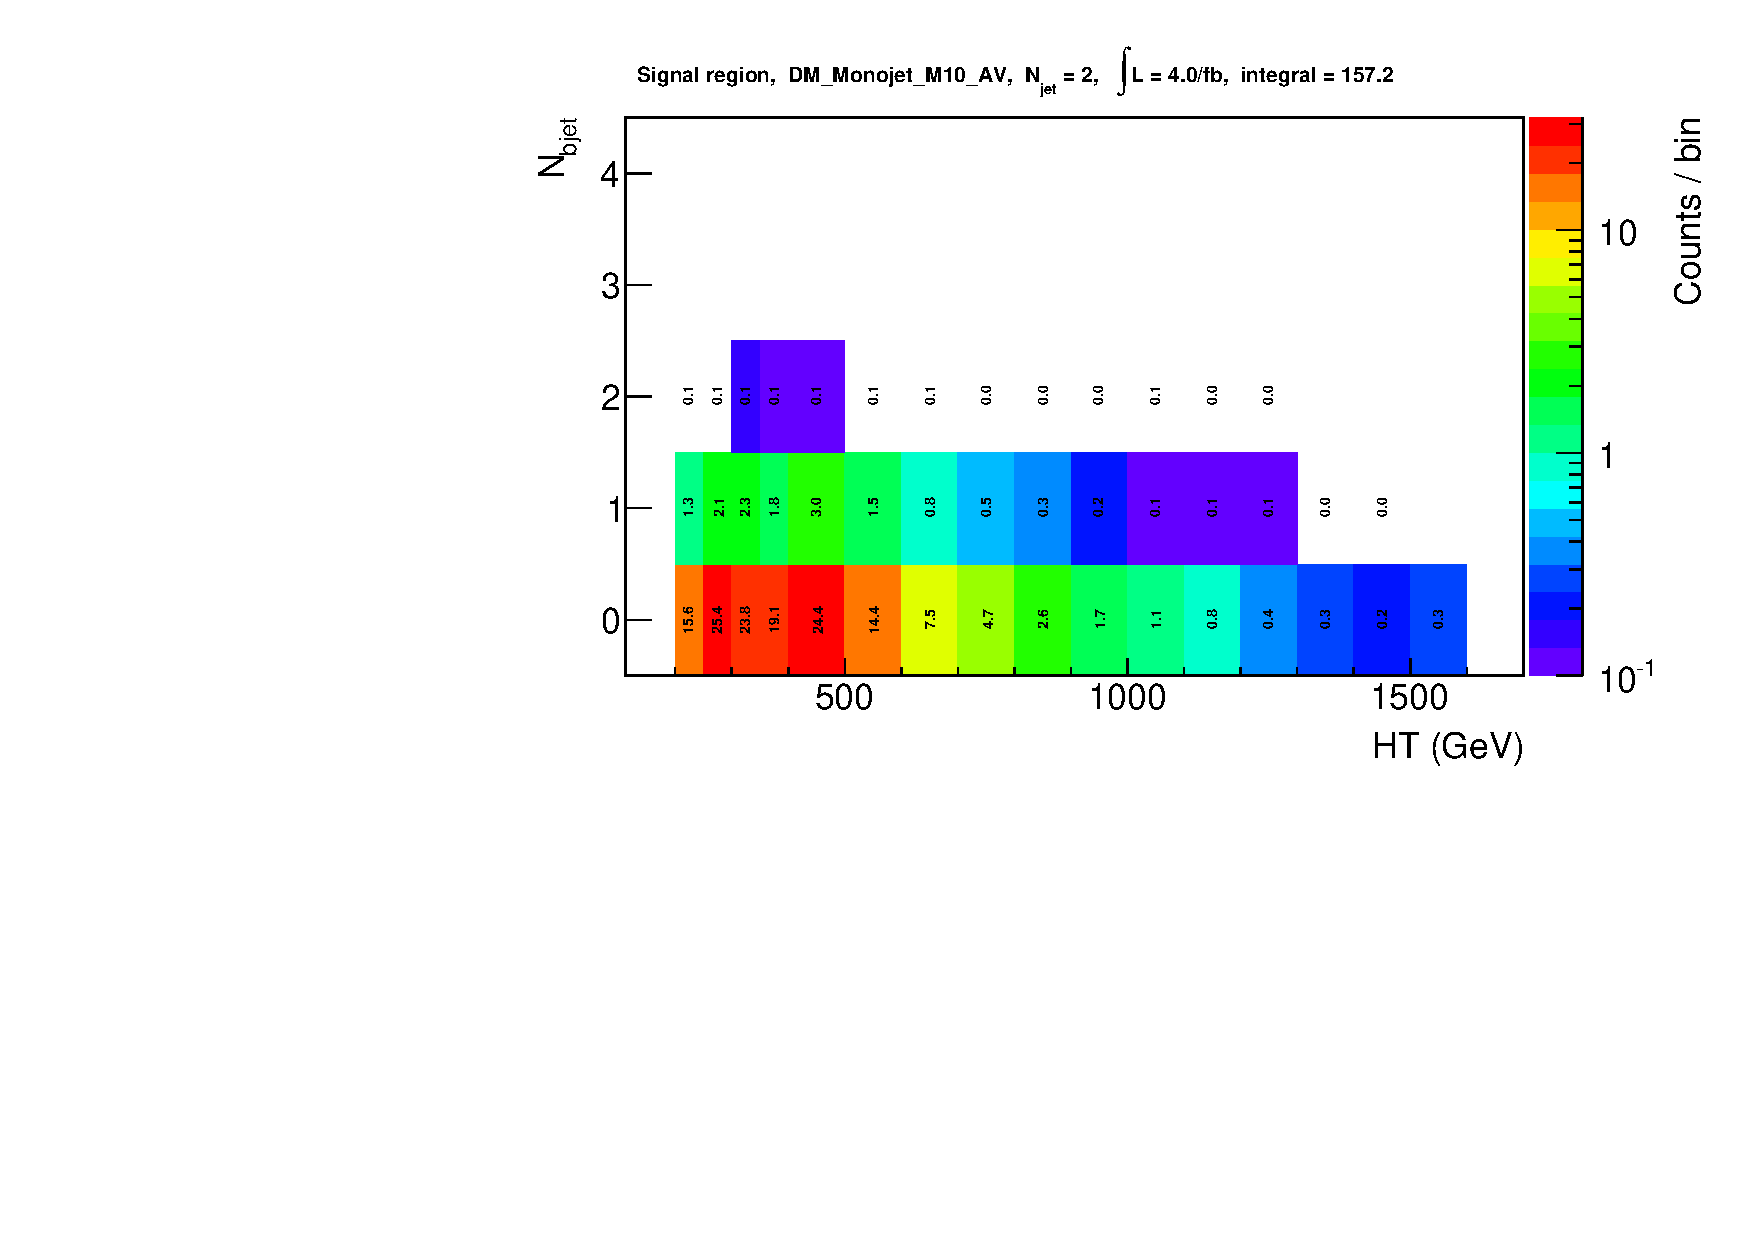
\includegraphics[width=0.5\textwidth]{figures/yieldPlots/sig_DM_Monojet_M10_AV_eq2j.pdf}
  }~~
  \subfigure[Hadronic signal region yields for the axial vectorDM model, asymetric selection.
  ($\njet = 2$)]{
    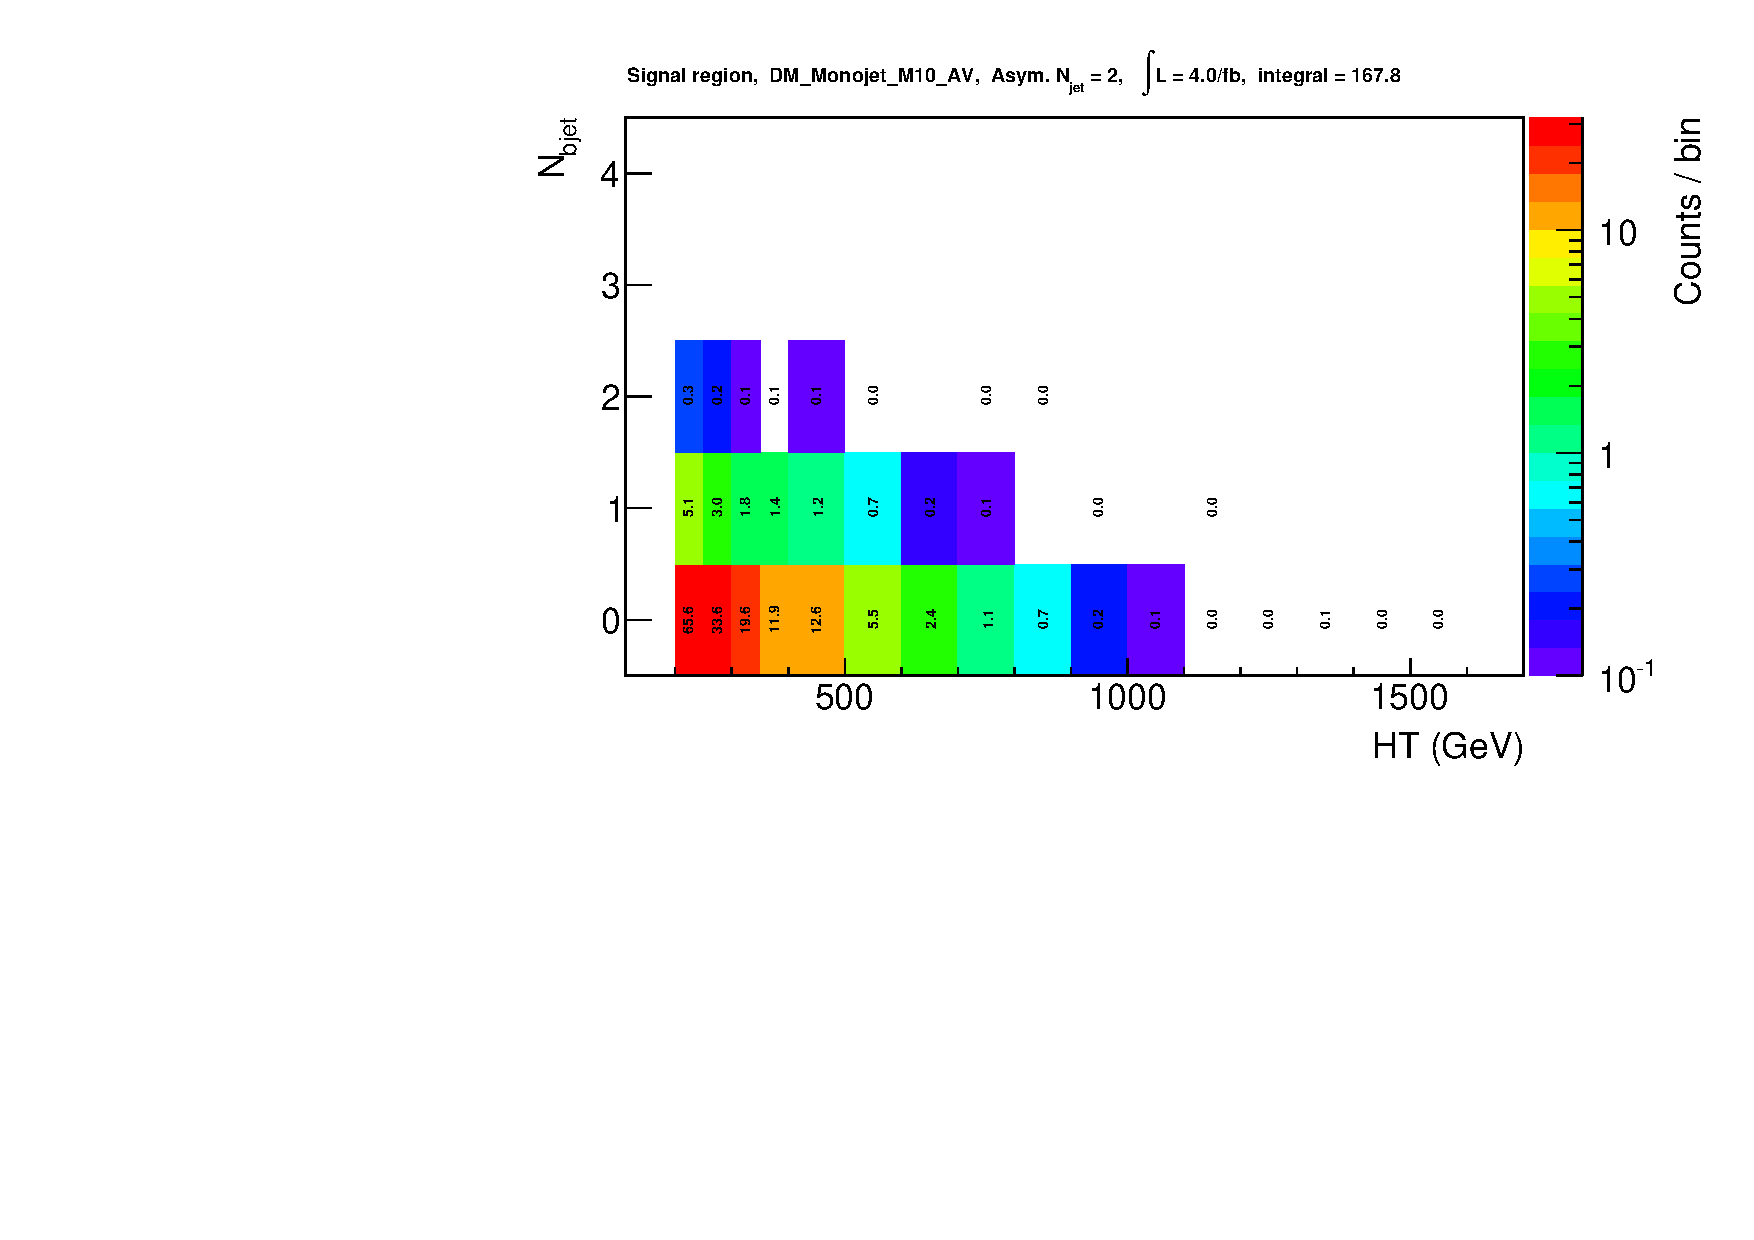
\includegraphics[width=0.5\textwidth]{figures/yieldPlots/sig_DM_Monojet_M10_AV_eq2jAsym.pdf}
  }\\

  \subfigure[Hadronic signal region yields for the axial vector DM model, nominal selection.
  ($\njet = 2$)]{
    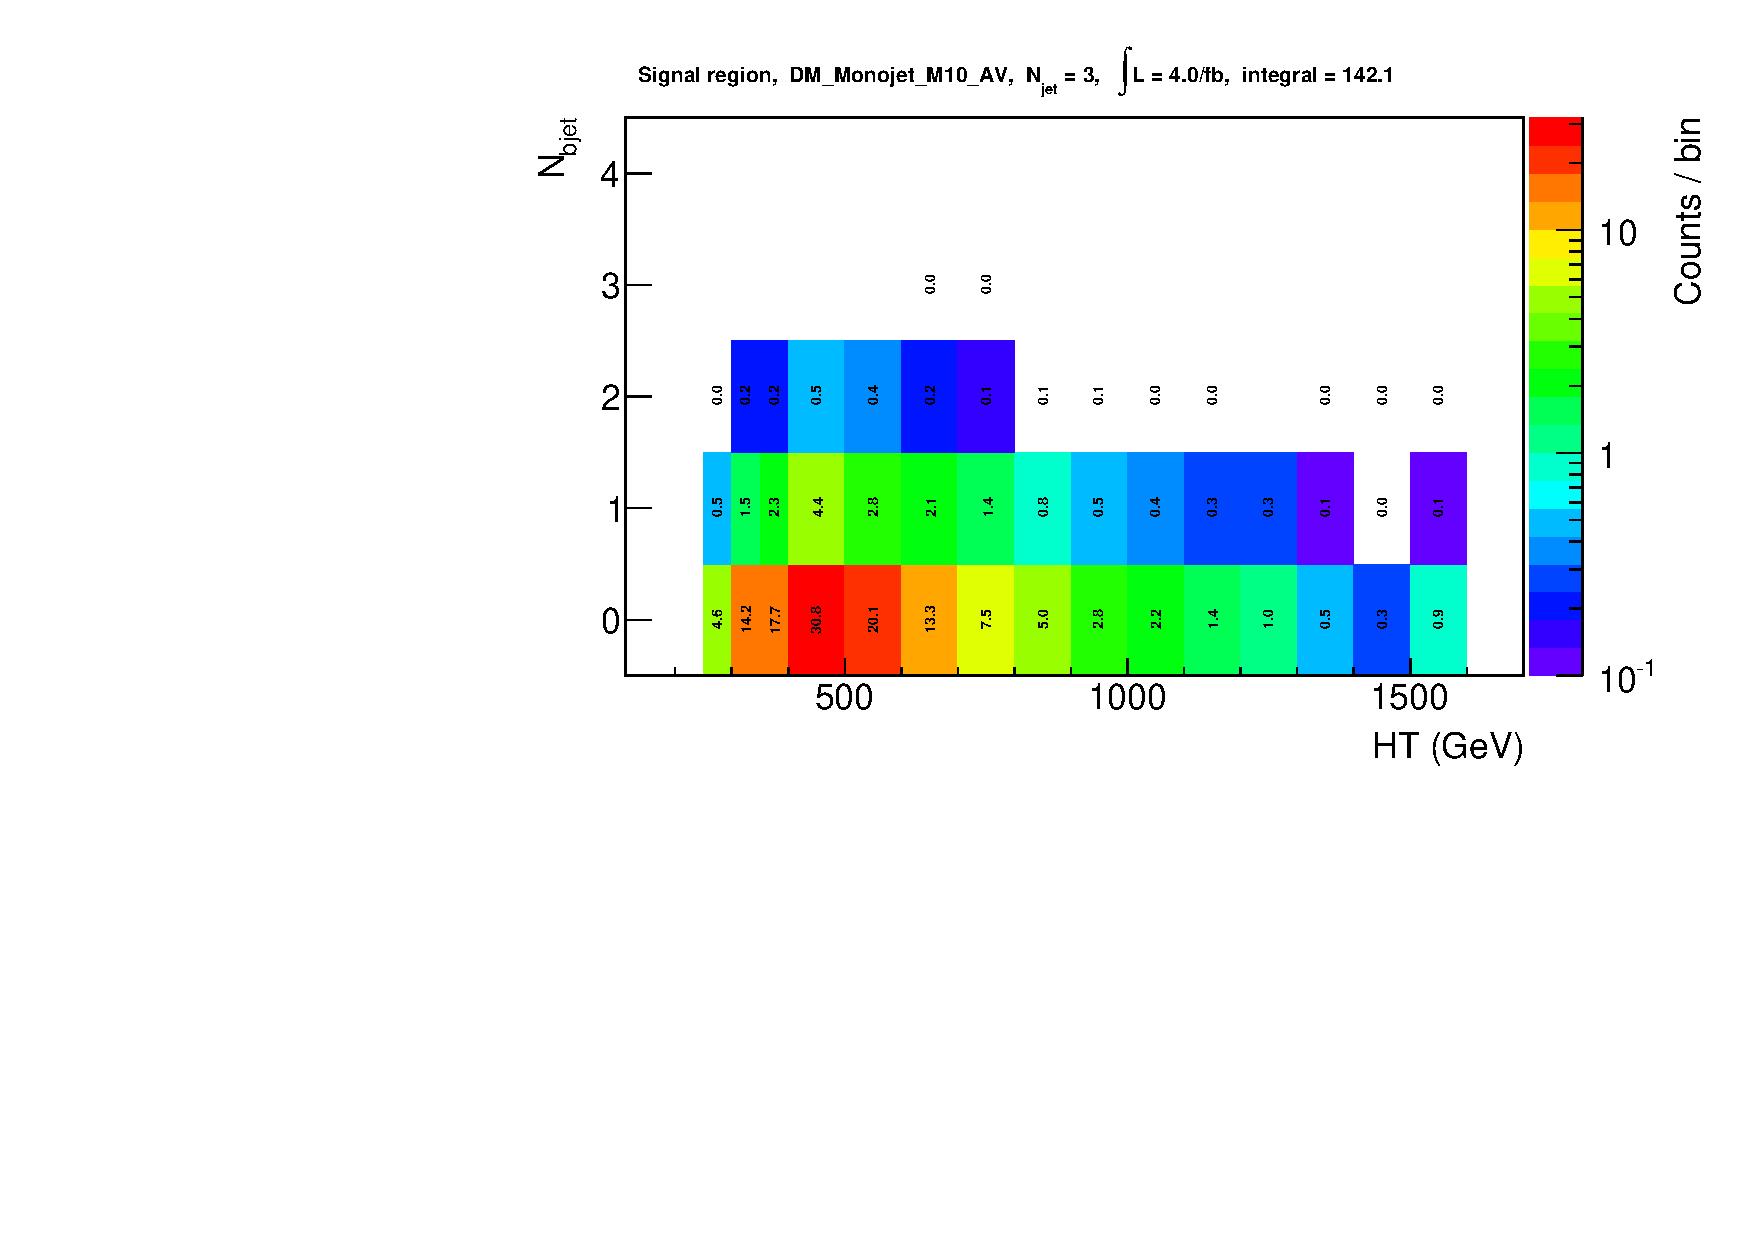
\includegraphics[width=0.5\textwidth]{figures/yieldPlots/sig_DM_Monojet_M10_AV_eq3j.pdf}
  }~~
  \subfigure[Hadronic signal region yields for the axial vectorDM model, asymetric selection.
  ($\njet = 2$)]{
    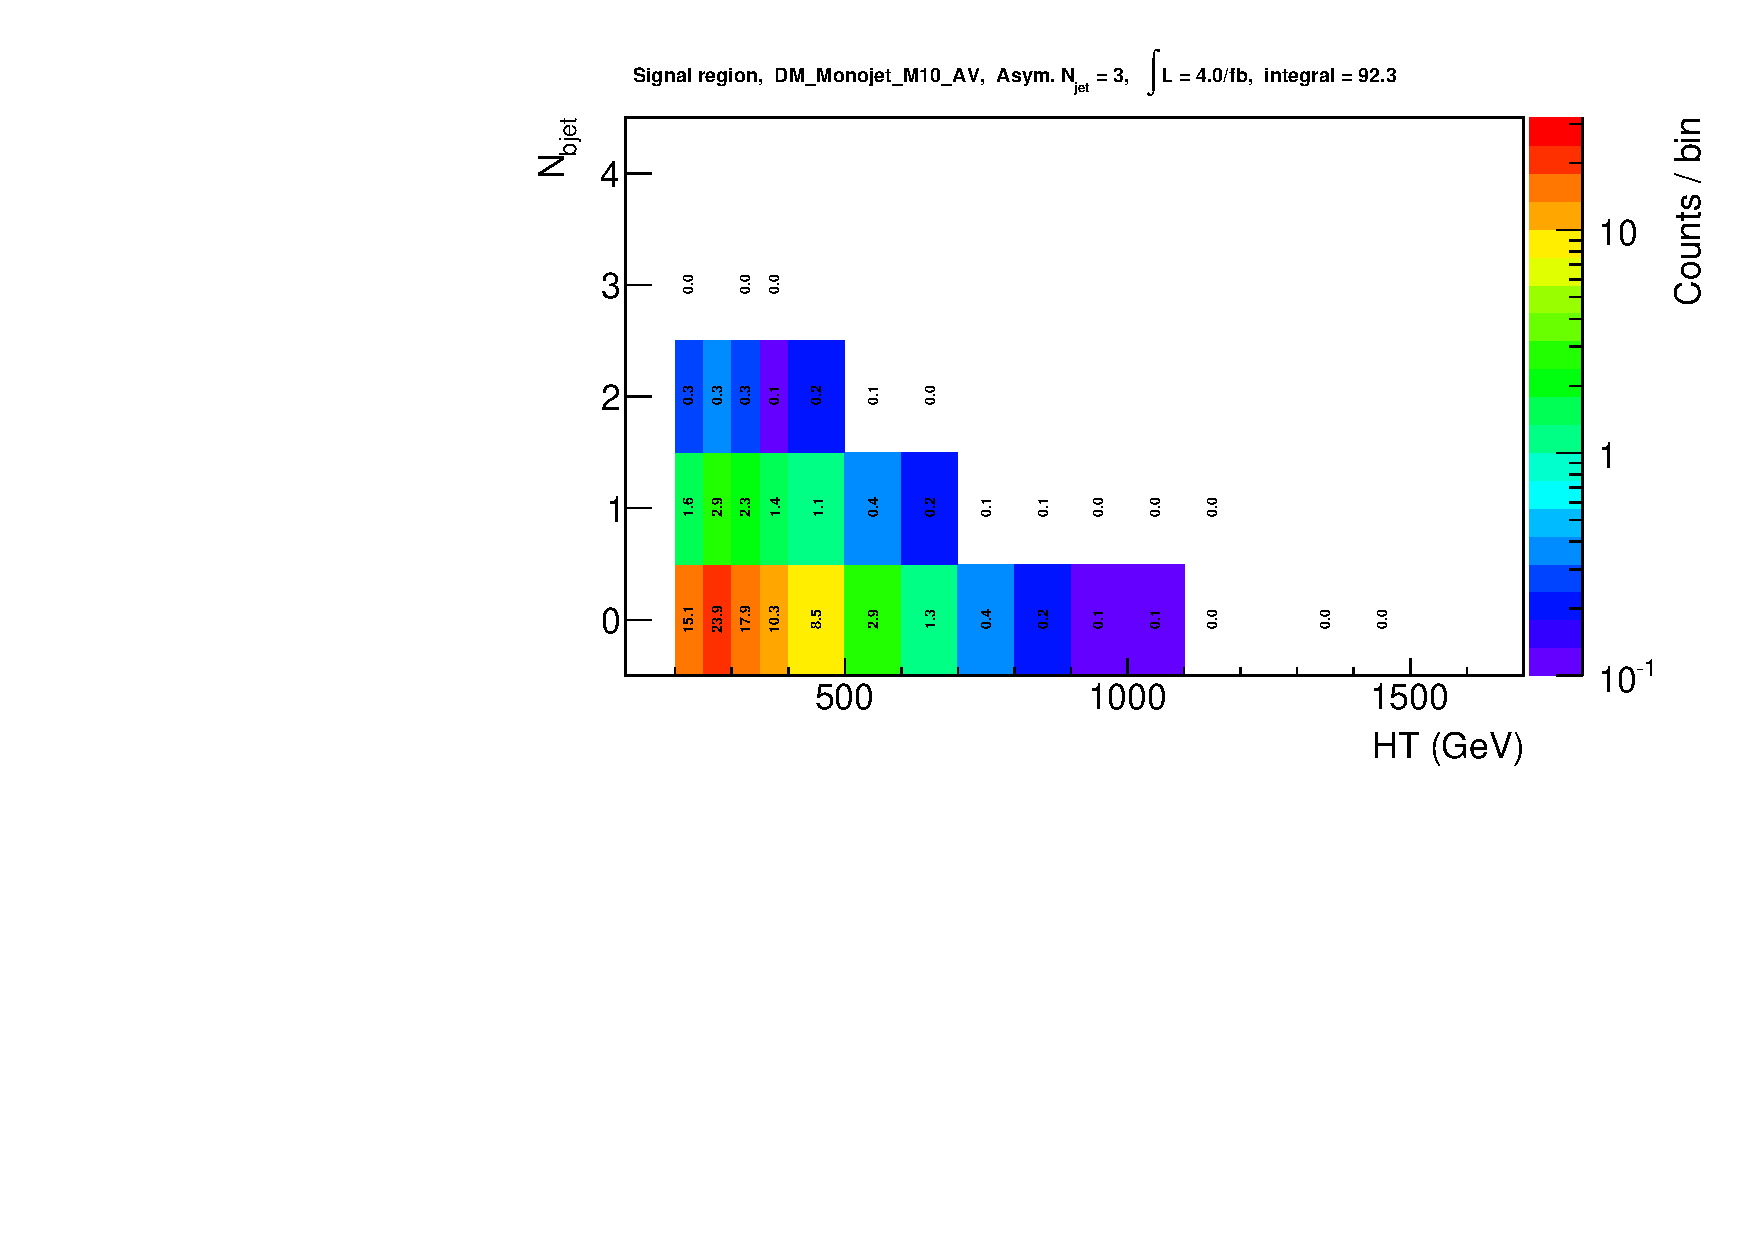
\includegraphics[width=0.5\textwidth]{figures/yieldPlots/sig_DM_Monojet_M10_AV_eq3jAsym.pdf}
  }\\
  \caption{\label{fig:DM_AV_Yields1} Yields at $4\fbinv$ for the AV DM model in the
  hadronic signal region, for $\njet=2,3$. The binning corresponds to the analysis  bins. }
\end{figure}



\begin{figure}[]
  \centering
  \subfigure[Hadronic signal region yields for the axial vector DM model, nominal selection.
  ($\njet = 2$)]{
    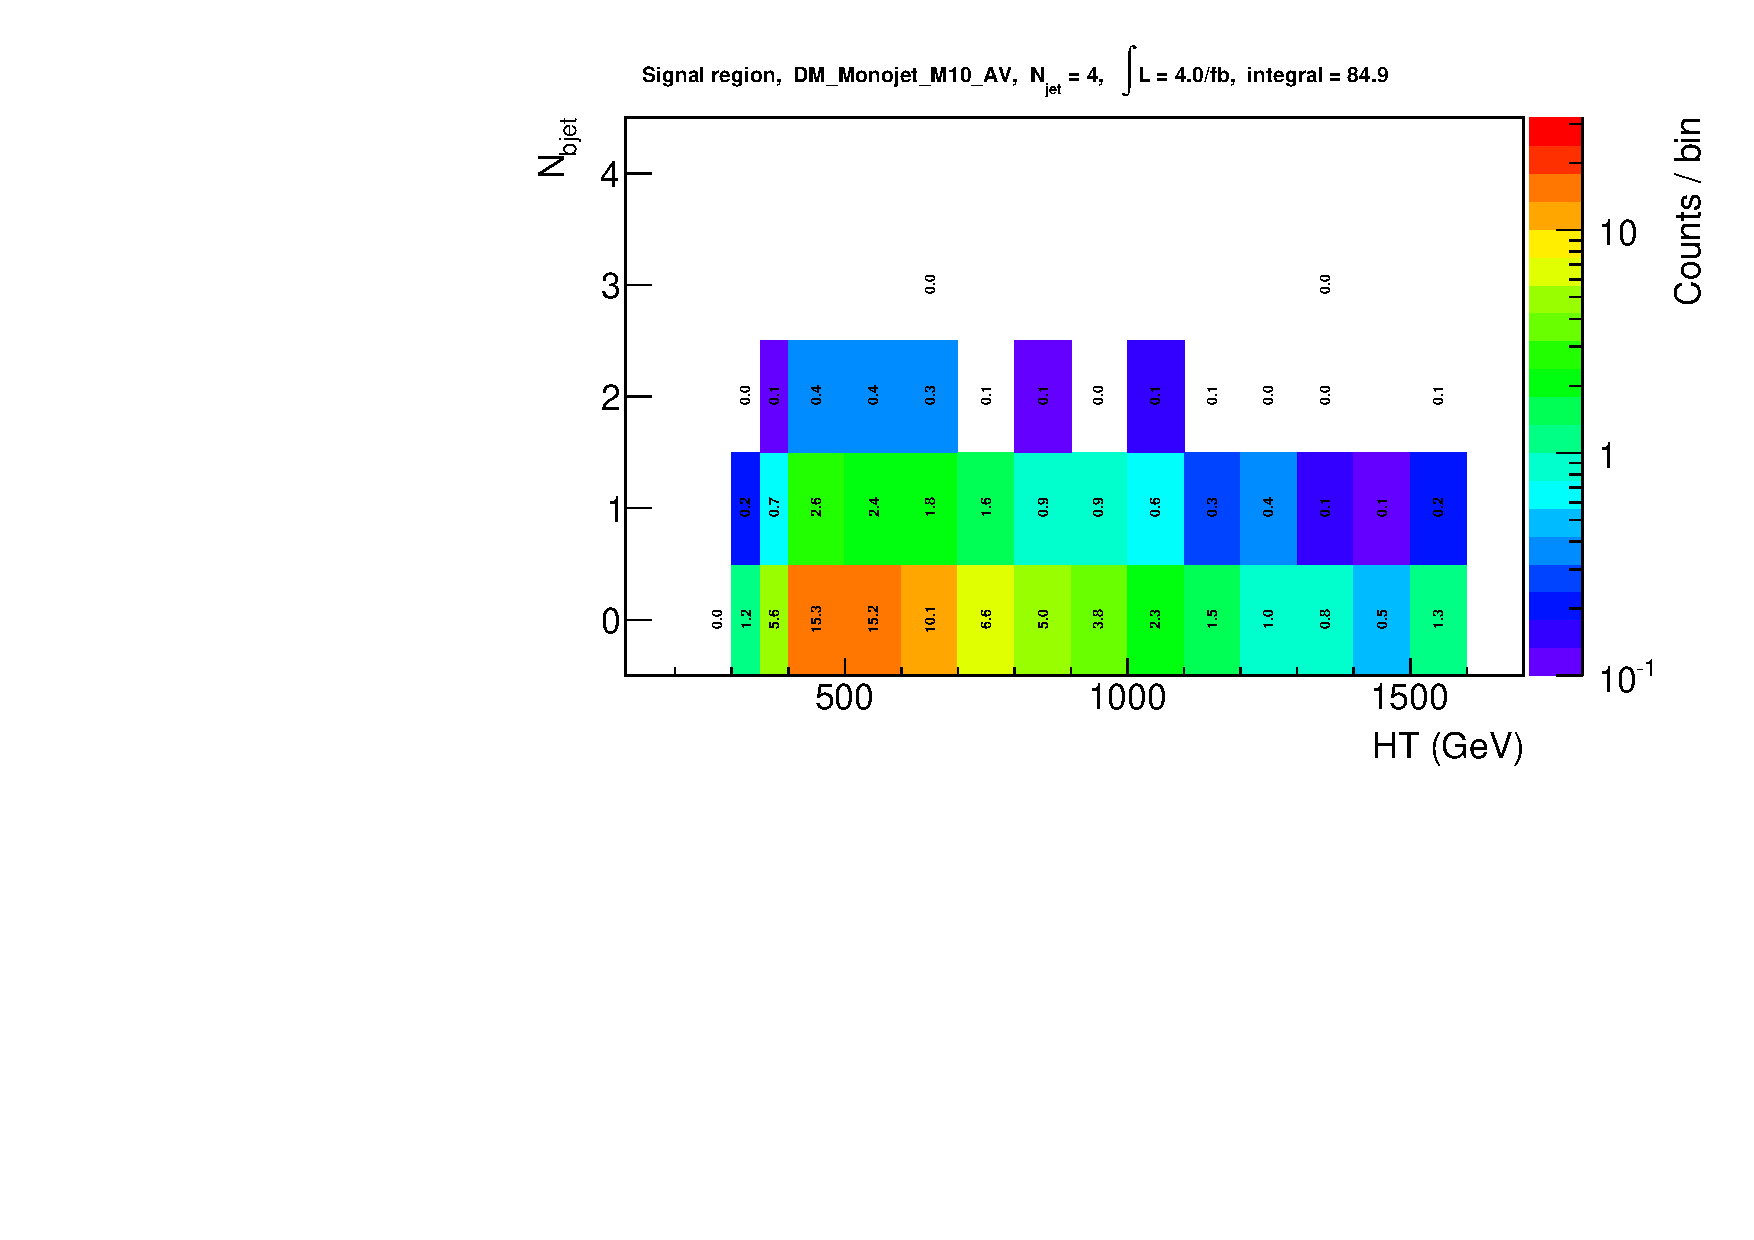
\includegraphics[width=0.5\textwidth]{figures/yieldPlots/sig_DM_Monojet_M10_AV_eq4j.pdf}
  }~~
  \subfigure[Hadronic signal region yields for the axial vectorDM model, asymetric selection.
  ($\njet = 2$)]{
    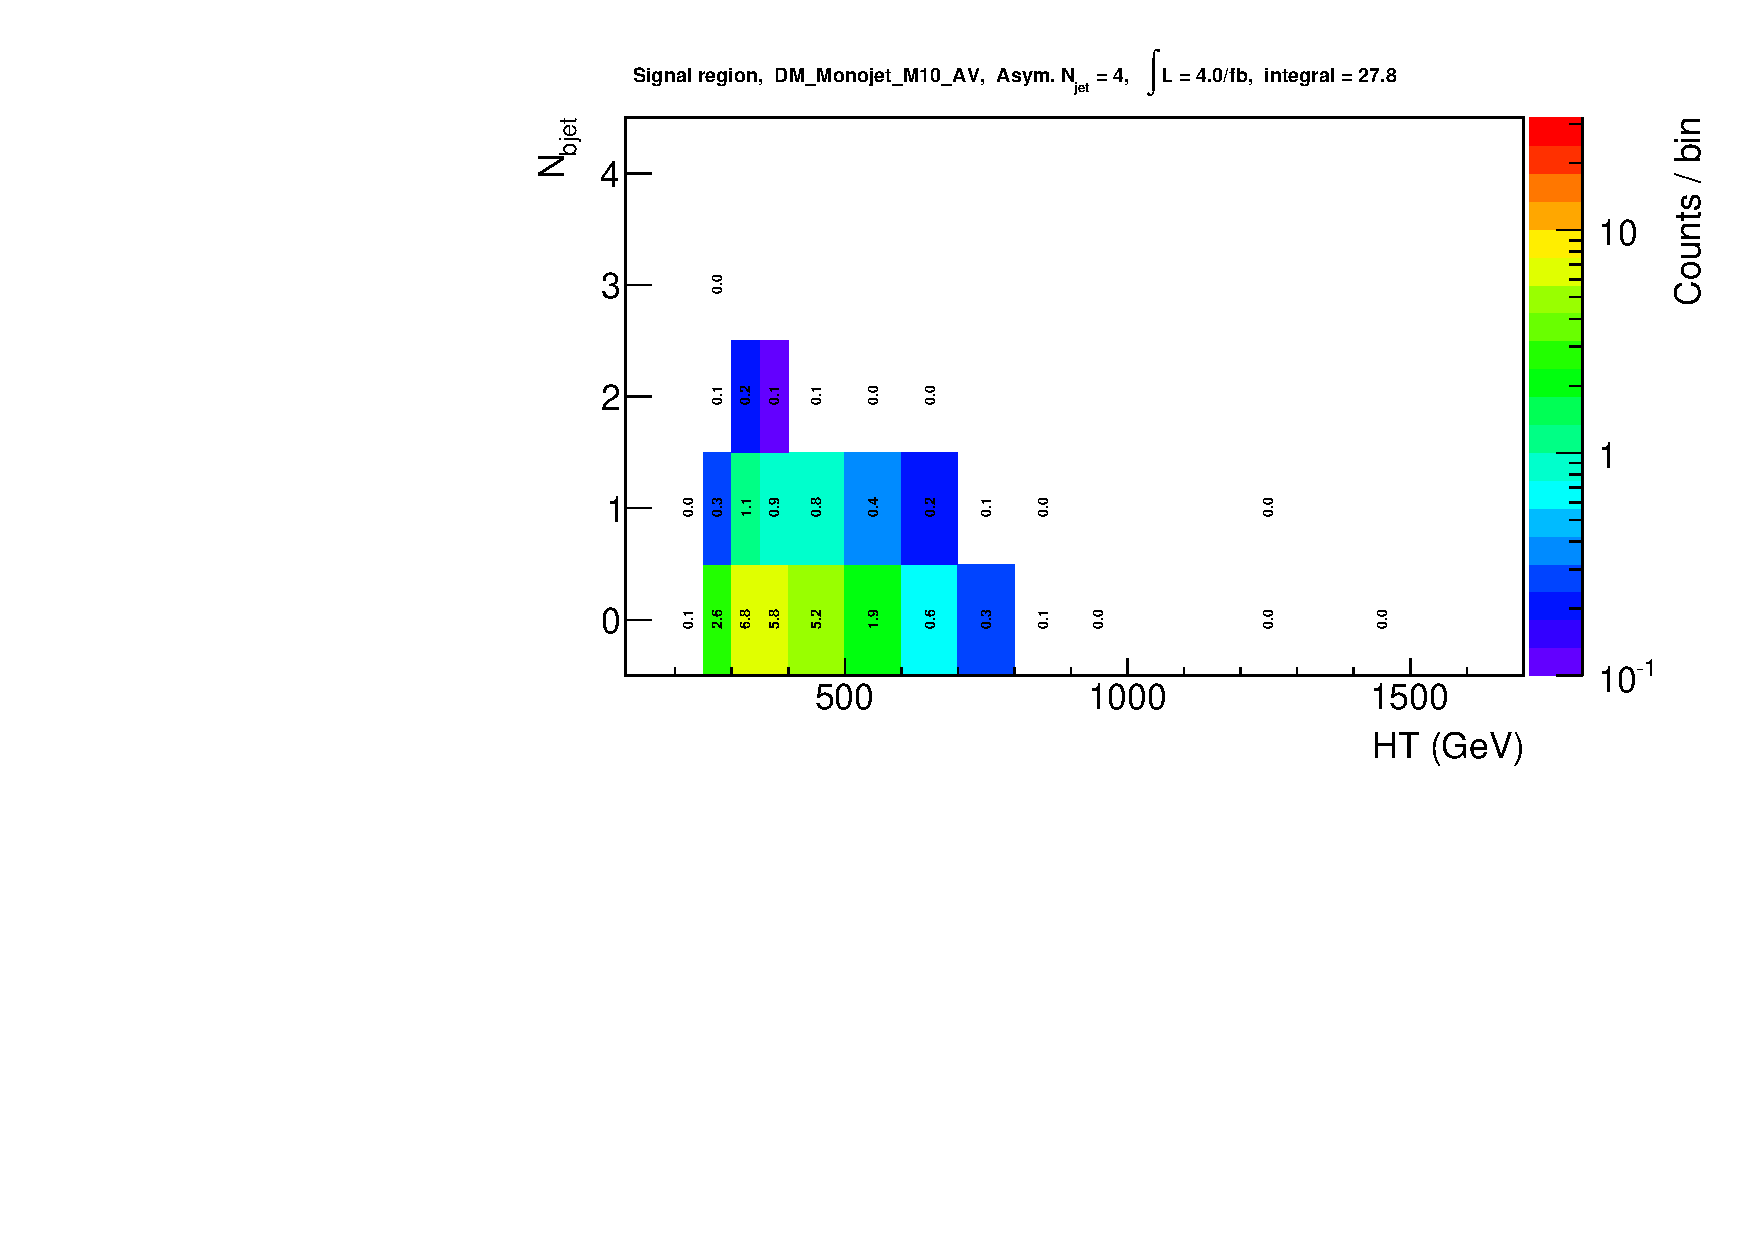
\includegraphics[width=0.5\textwidth]{figures/yieldPlots/sig_DM_Monojet_M10_AV_eq4jAsym.pdf}
  }\\

  \subfigure[Hadronic signal region yields for the axial vector DM model, nominal selection.
  ($\njet = 5$)]{
    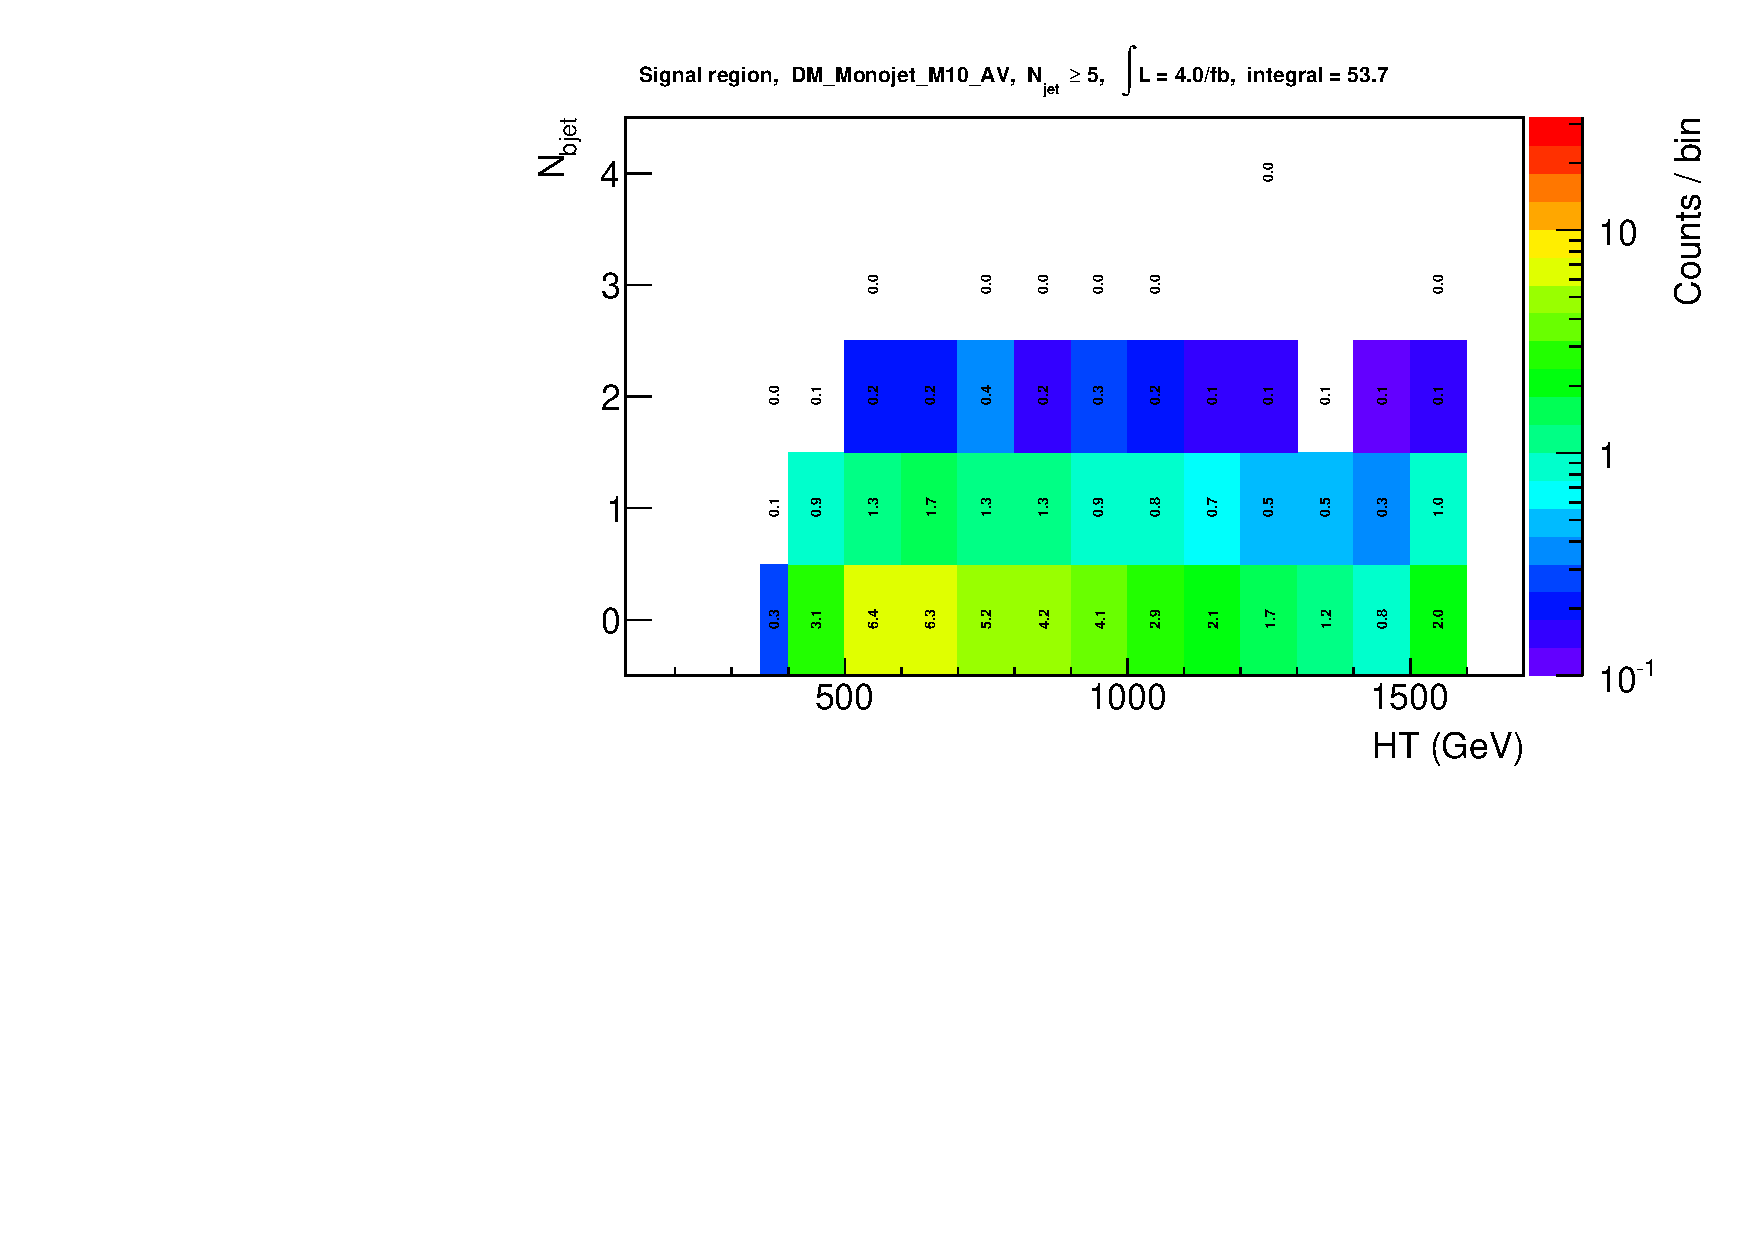
\includegraphics[width=0.5\textwidth]{figures/yieldPlots/sig_DM_Monojet_M10_AV_ge5j.pdf}
  }~~
  \subfigure[Hadronic signal region yields for the axial vectorDM model, asymetric selection.
  ($\njet = 5$)]{
    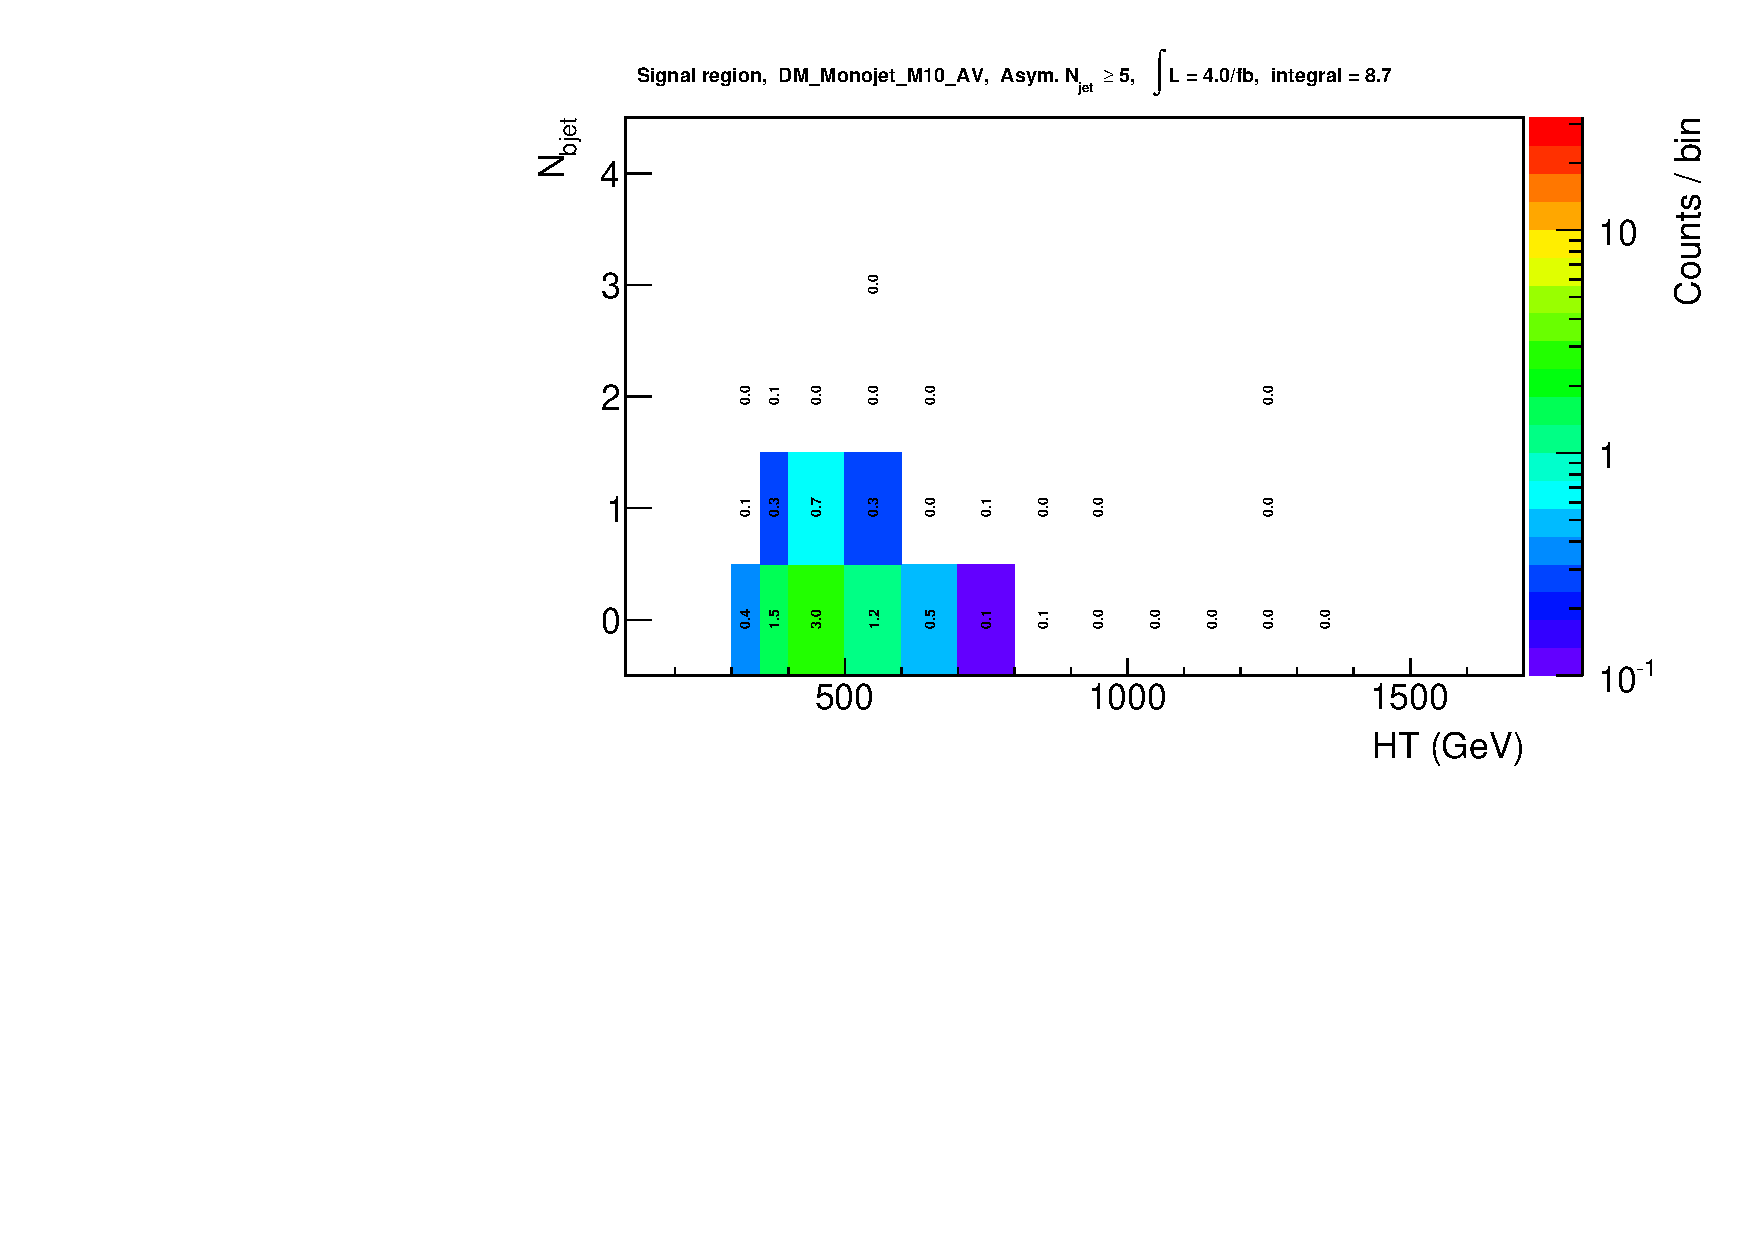
\includegraphics[width=0.5\textwidth]{figures/yieldPlots/sig_DM_Monojet_M10_AV_ge5jAsym.pdf}
  }
  \caption{\label{fig:DM_AV_Yields2} Yields at $4\fbinv$ for the AV DM in the
  hadronic signal region, for $\njet=4,5$. The binning corresponds to the analysis  bins. }
\end{figure}




\begin{figure}[]
  \centering
  \subfigure[Hadronic signal region yields for the axial vector DM model, nominal selection.
  ($\njet = 2$)]{
    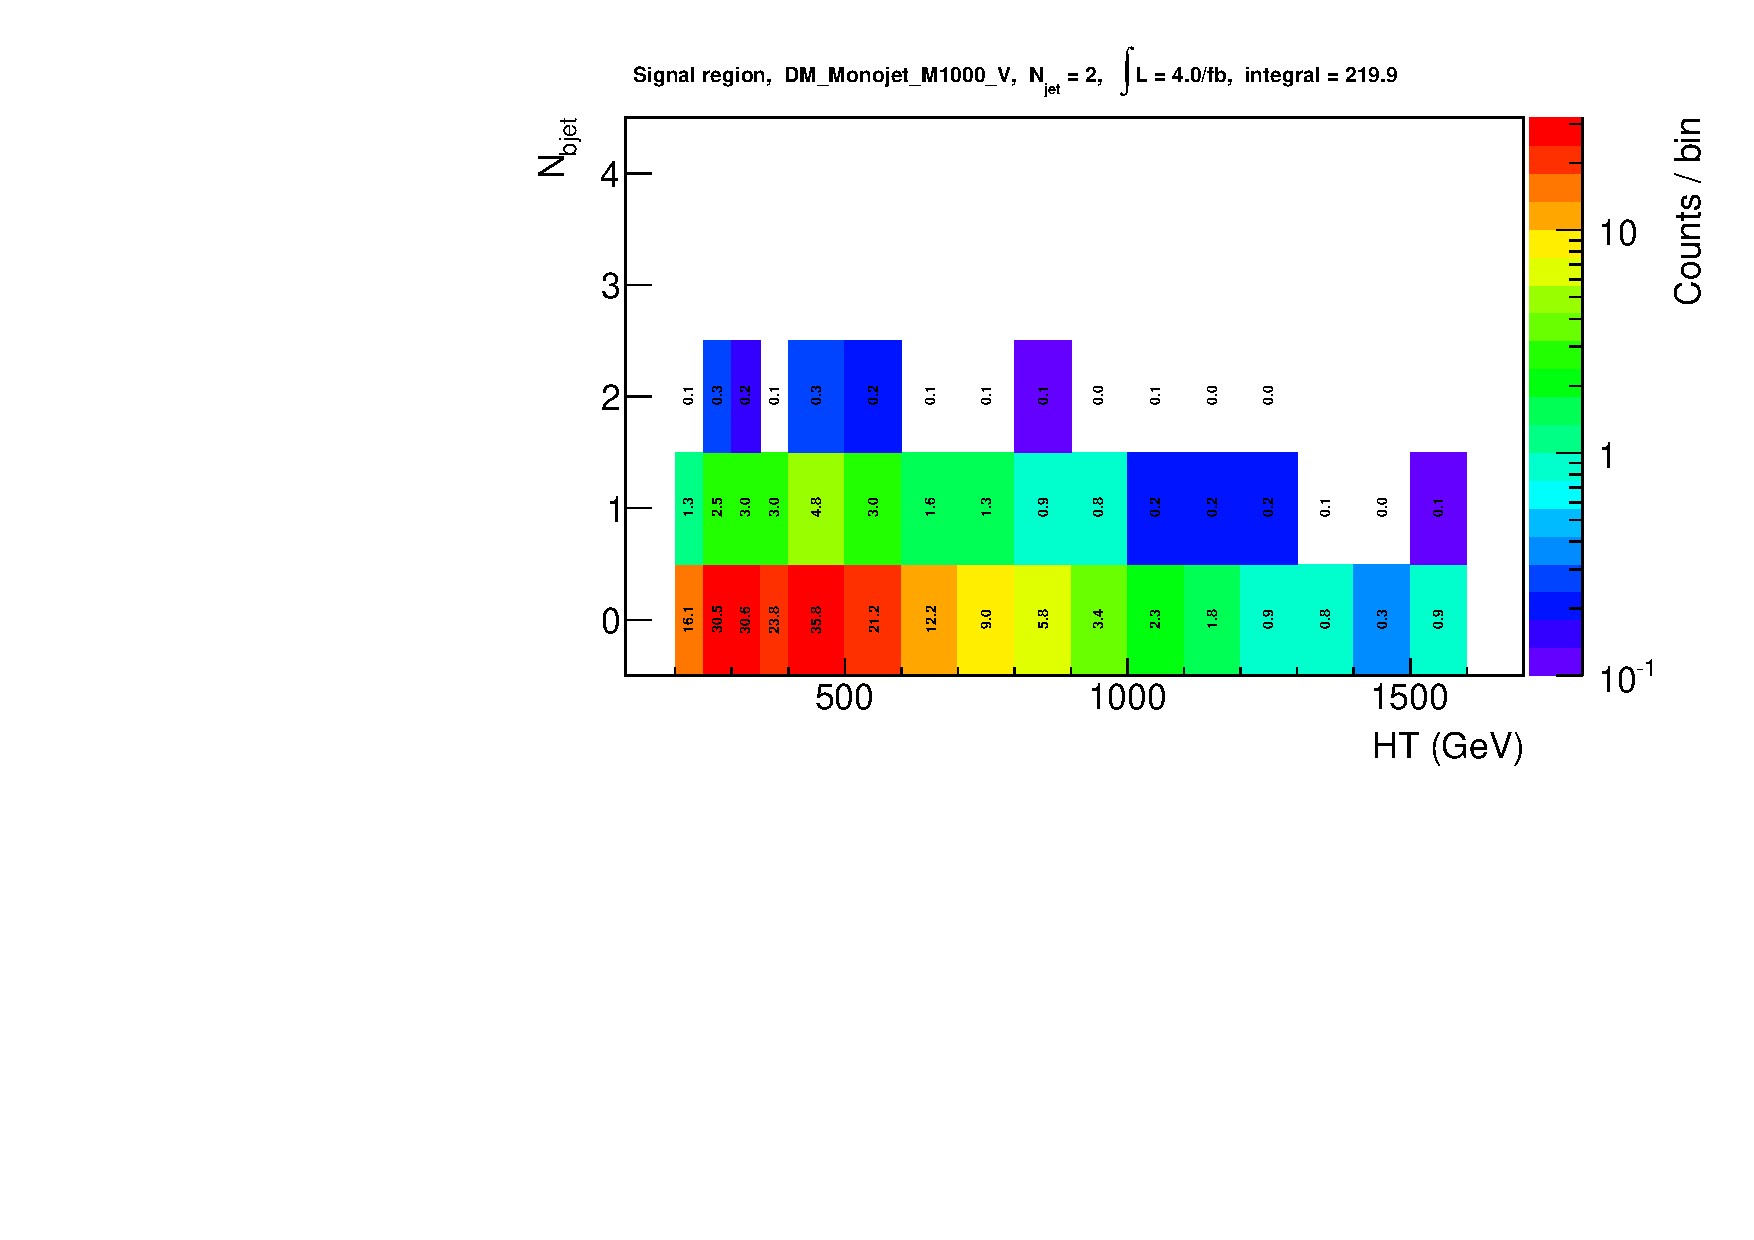
\includegraphics[width=0.5\textwidth]{figures/yieldPlots/sig_DM_Monojet_M1000_V_eq2j.pdf}
  }~~
  \subfigure[Hadronic signal region yields for the axial vectorDM model, asymetric selection.
  ($\njet = 2$)]{
    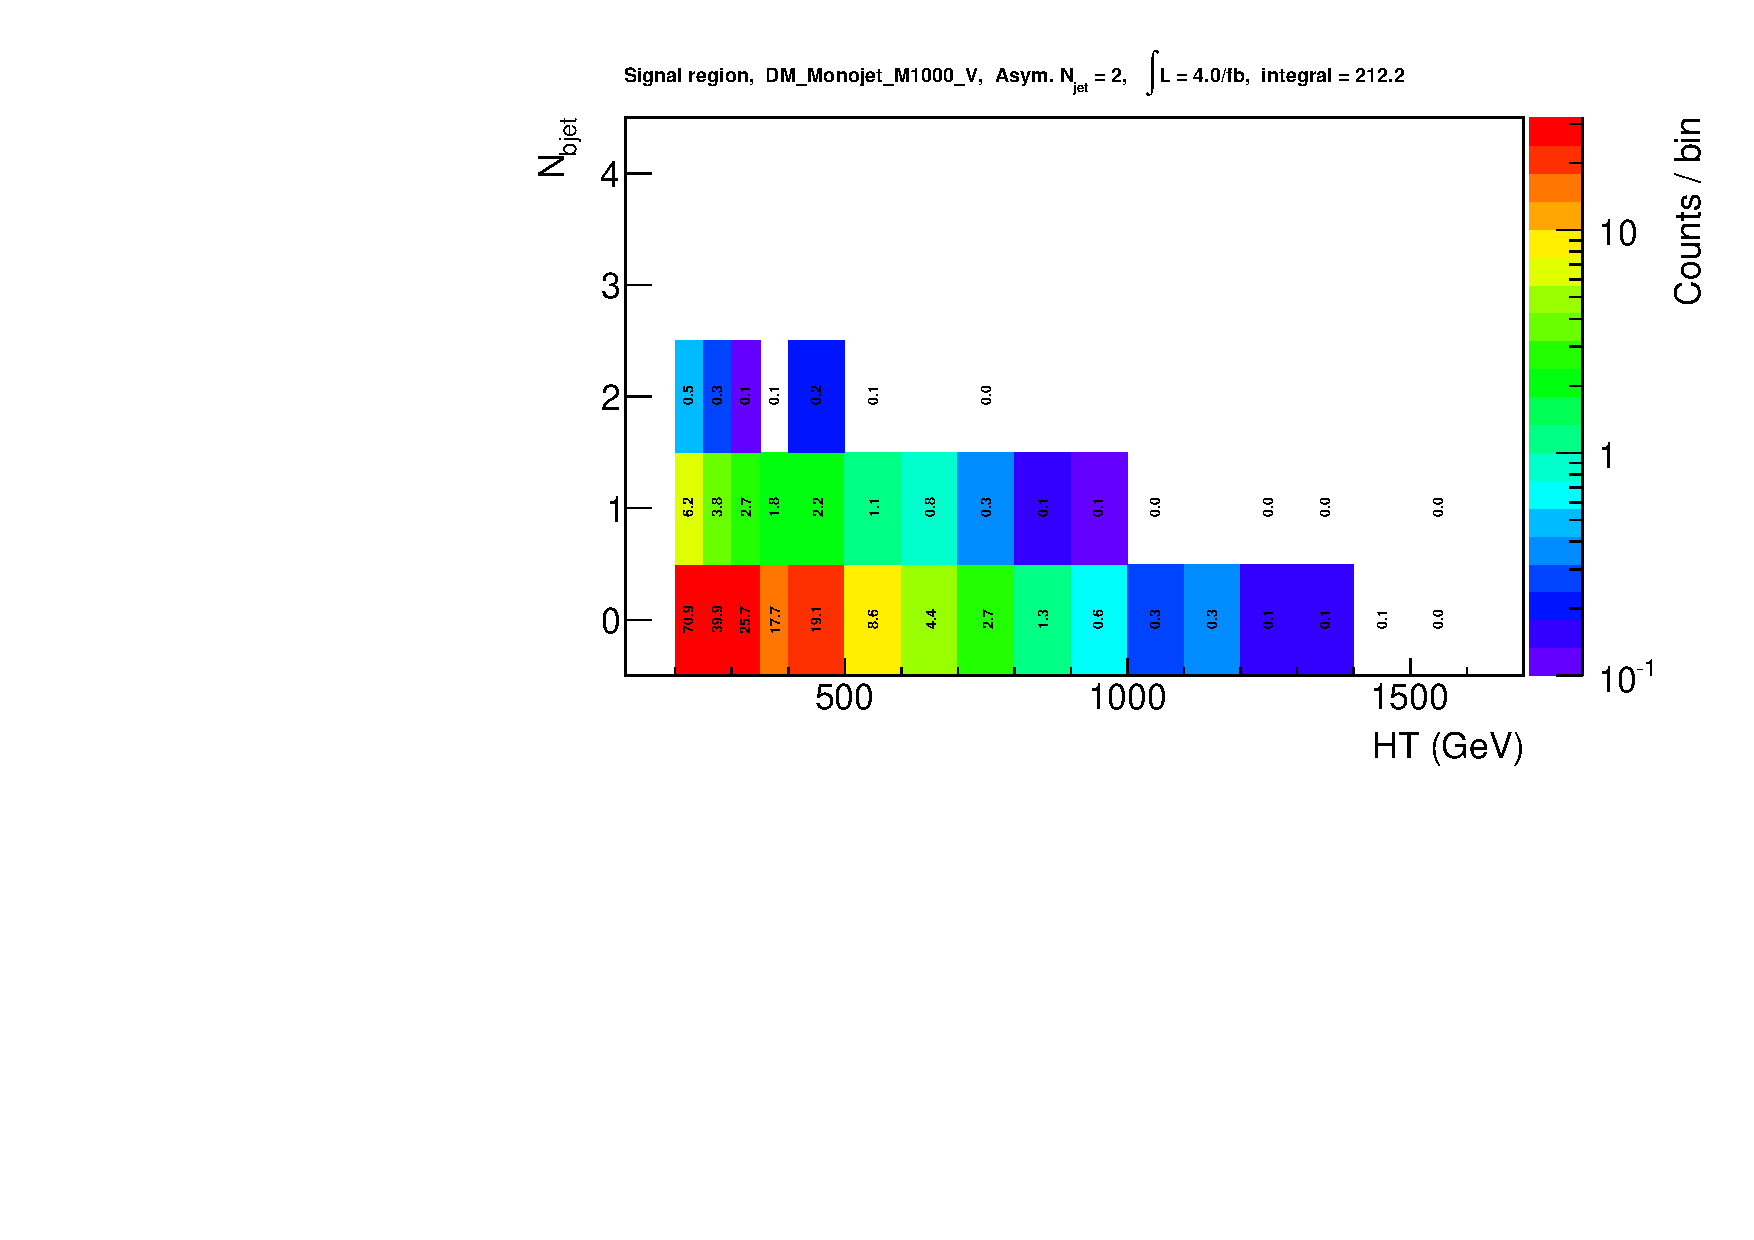
\includegraphics[width=0.5\textwidth]{figures/yieldPlots/sig_DM_Monojet_M1000_V_eq2jAsym.pdf}
  }\\

  \subfigure[Hadronic signal region yields for the axial vector DM model, nominal selection.
  ($\njet = 2$)]{
    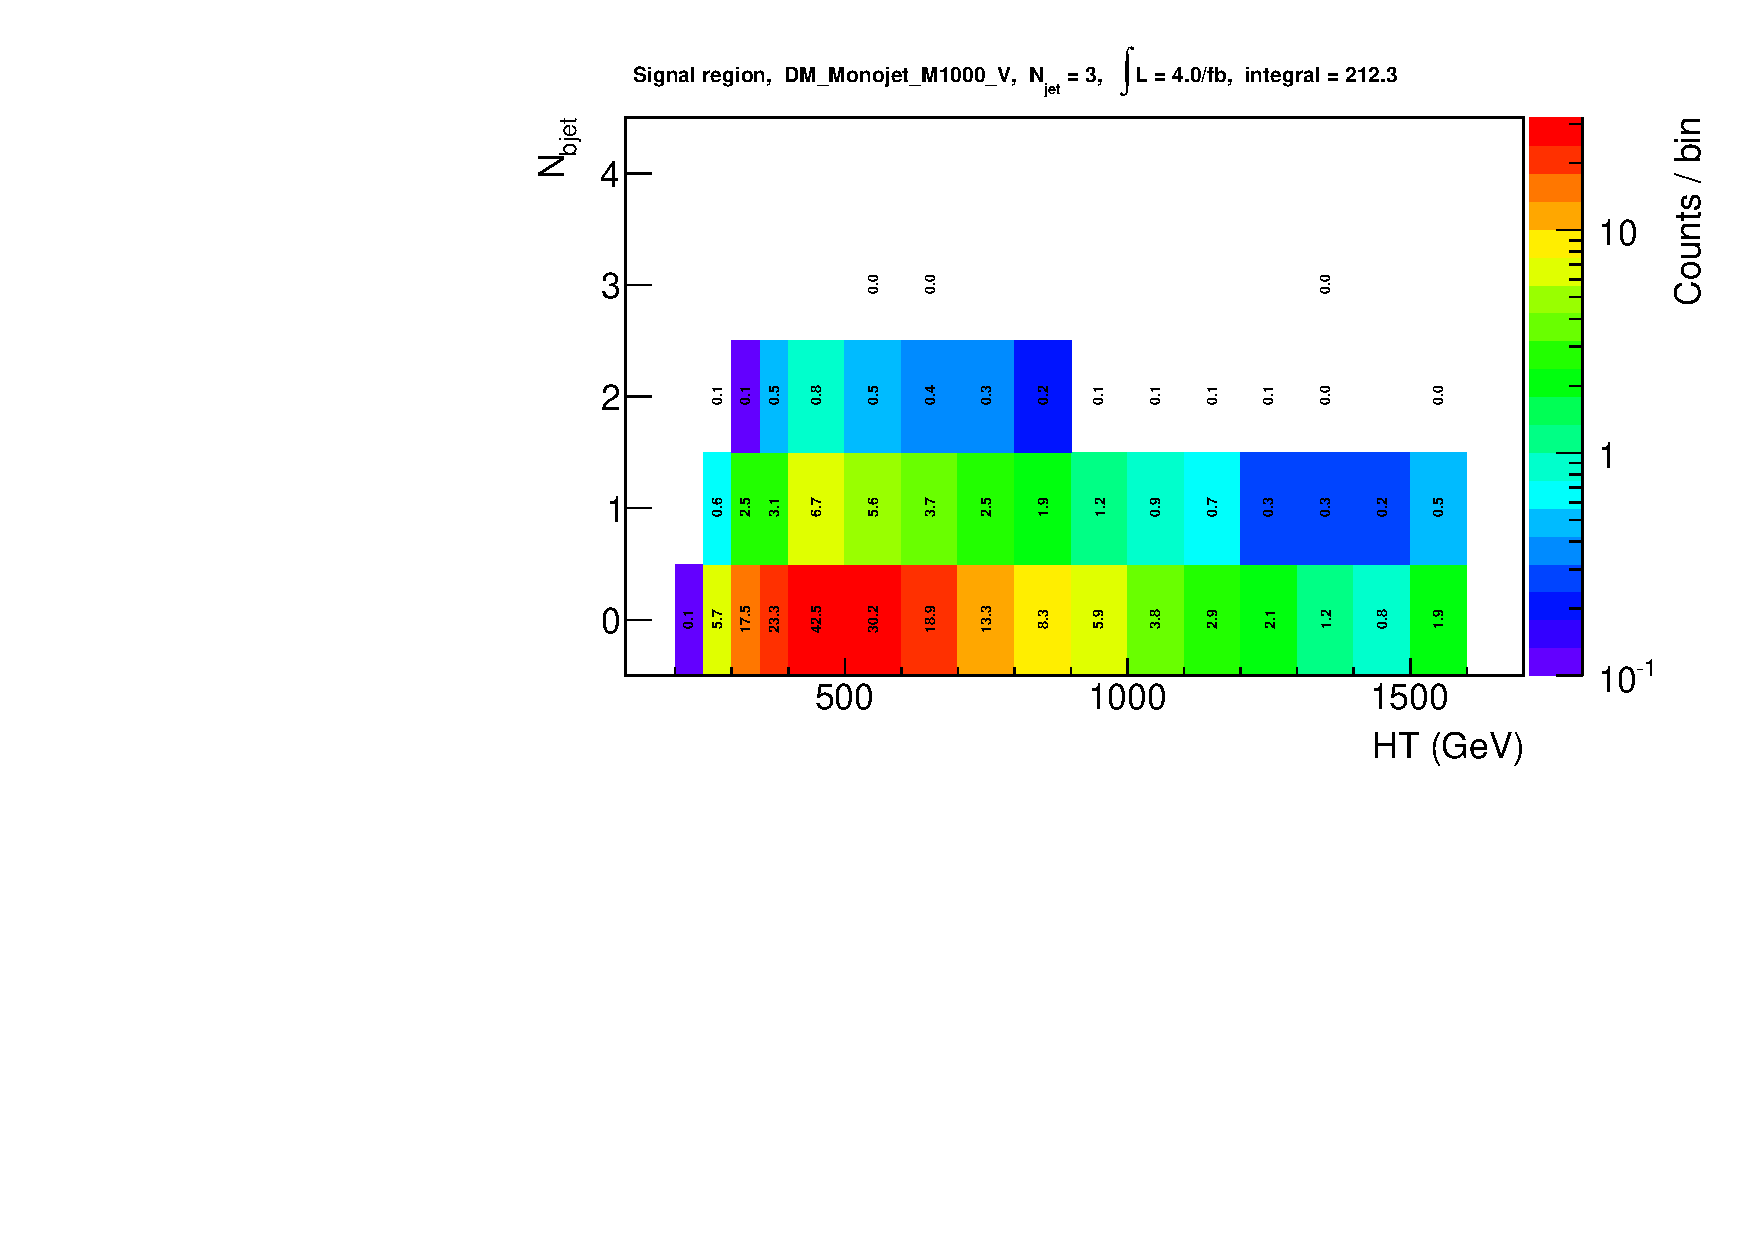
\includegraphics[width=0.5\textwidth]{figures/yieldPlots/sig_DM_Monojet_M1000_V_eq3j.pdf}
  }~~
  \subfigure[Hadronic signal region yields for the axial vectorDM model, asymetric selection.
  ($\njet = 2$)]{
    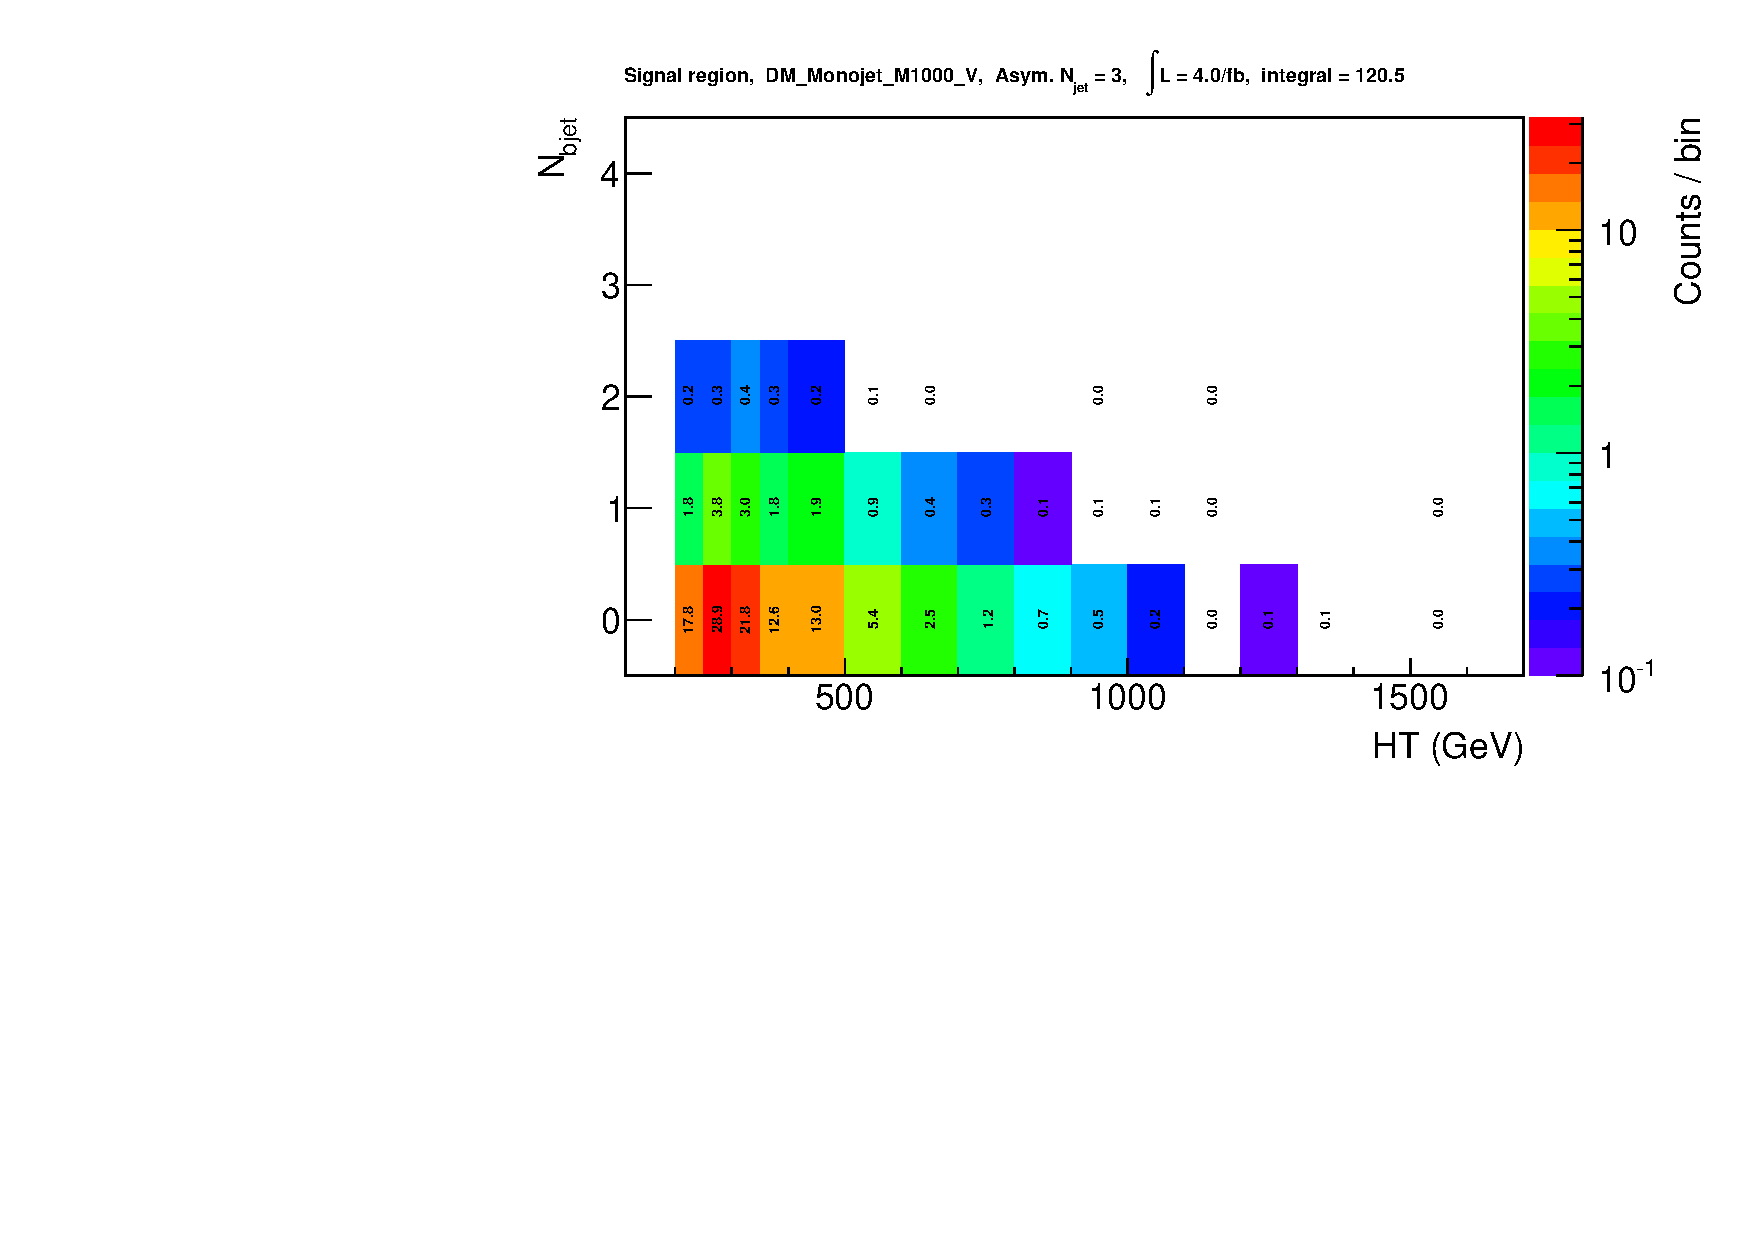
\includegraphics[width=0.5\textwidth]{figures/yieldPlots/sig_DM_Monojet_M1000_V_eq3jAsym.pdf}
  }\\
  \caption{\label{fig:DM_V_Yields1} Yields at $4\fbinv$ for the AV DM model in the
  hadronic signal region, for $\njet=2,3$. The binning corresponds to the analysis  bins. }
\end{figure}



\begin{figure}[]
  \centering
  \subfigure[Hadronic signal region yields for the axial vector DM model, nominal selection.
  ($\njet = 2$)]{
    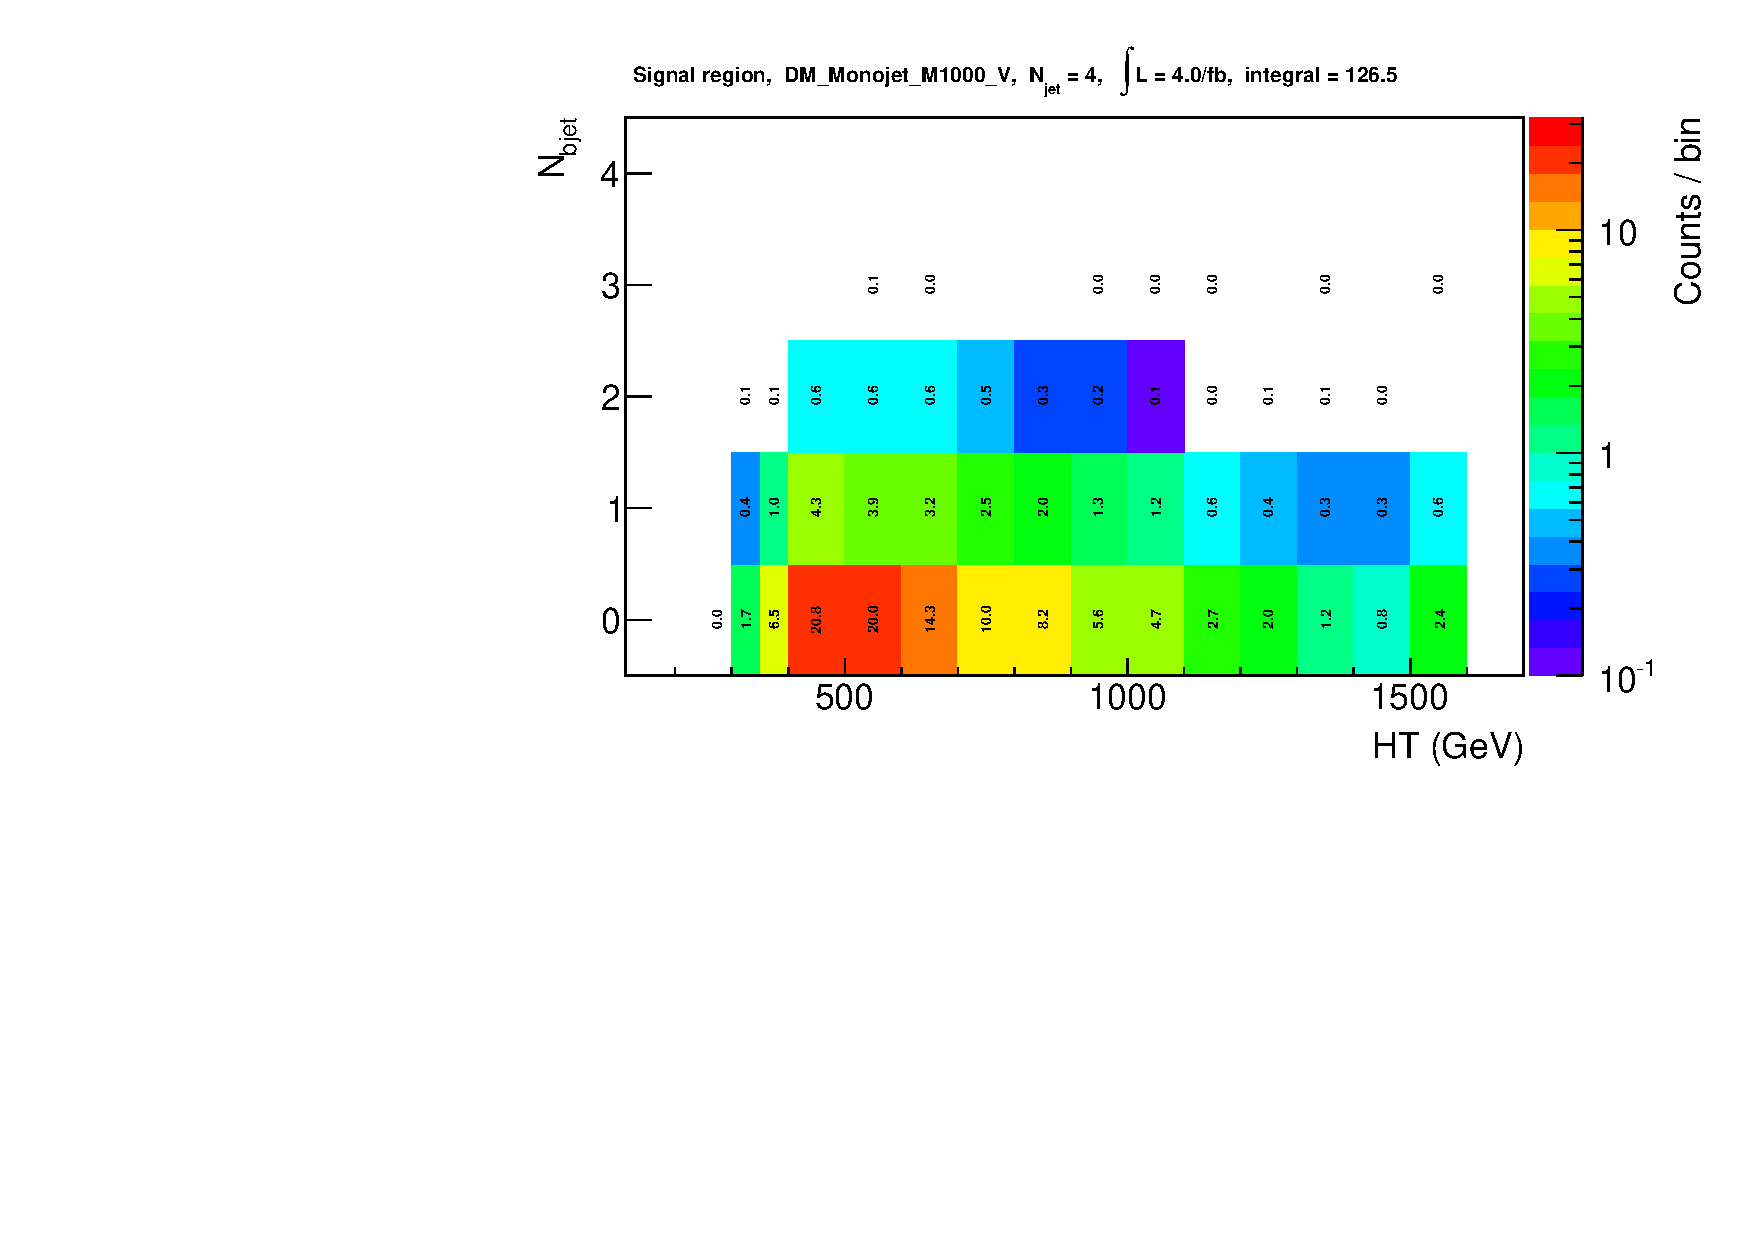
\includegraphics[width=0.5\textwidth]{figures/yieldPlots/sig_DM_Monojet_M1000_V_eq4j.pdf}
  }~~
  \subfigure[Hadronic signal region yields for the axial vectorDM model, asymetric selection.
  ($\njet = 2$)]{
    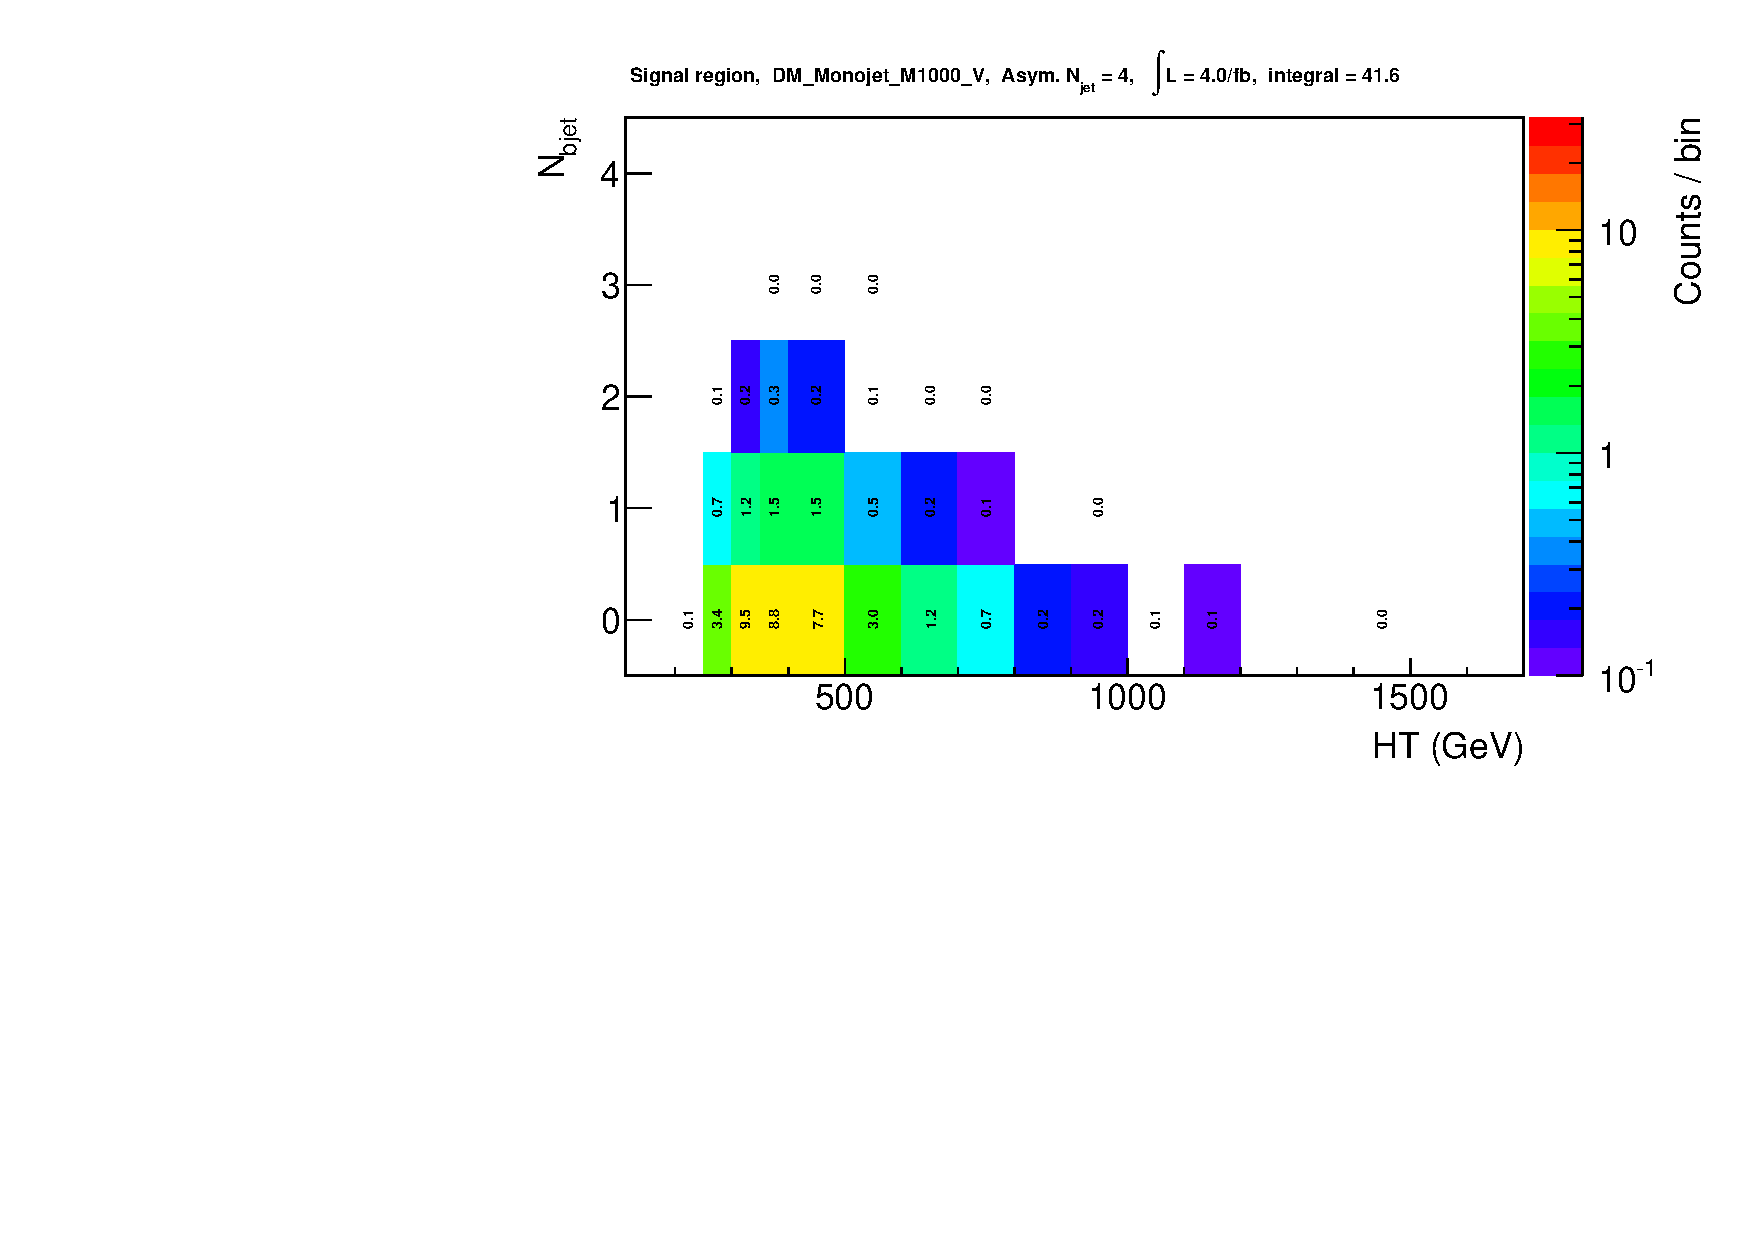
\includegraphics[width=0.5\textwidth]{figures/yieldPlots/sig_DM_Monojet_M1000_V_eq4jAsym.pdf}
  }\\

  \subfigure[Hadronic signal region yields for the axial vector DM model, nominal selection.
  ($\njet = 5$)]{
    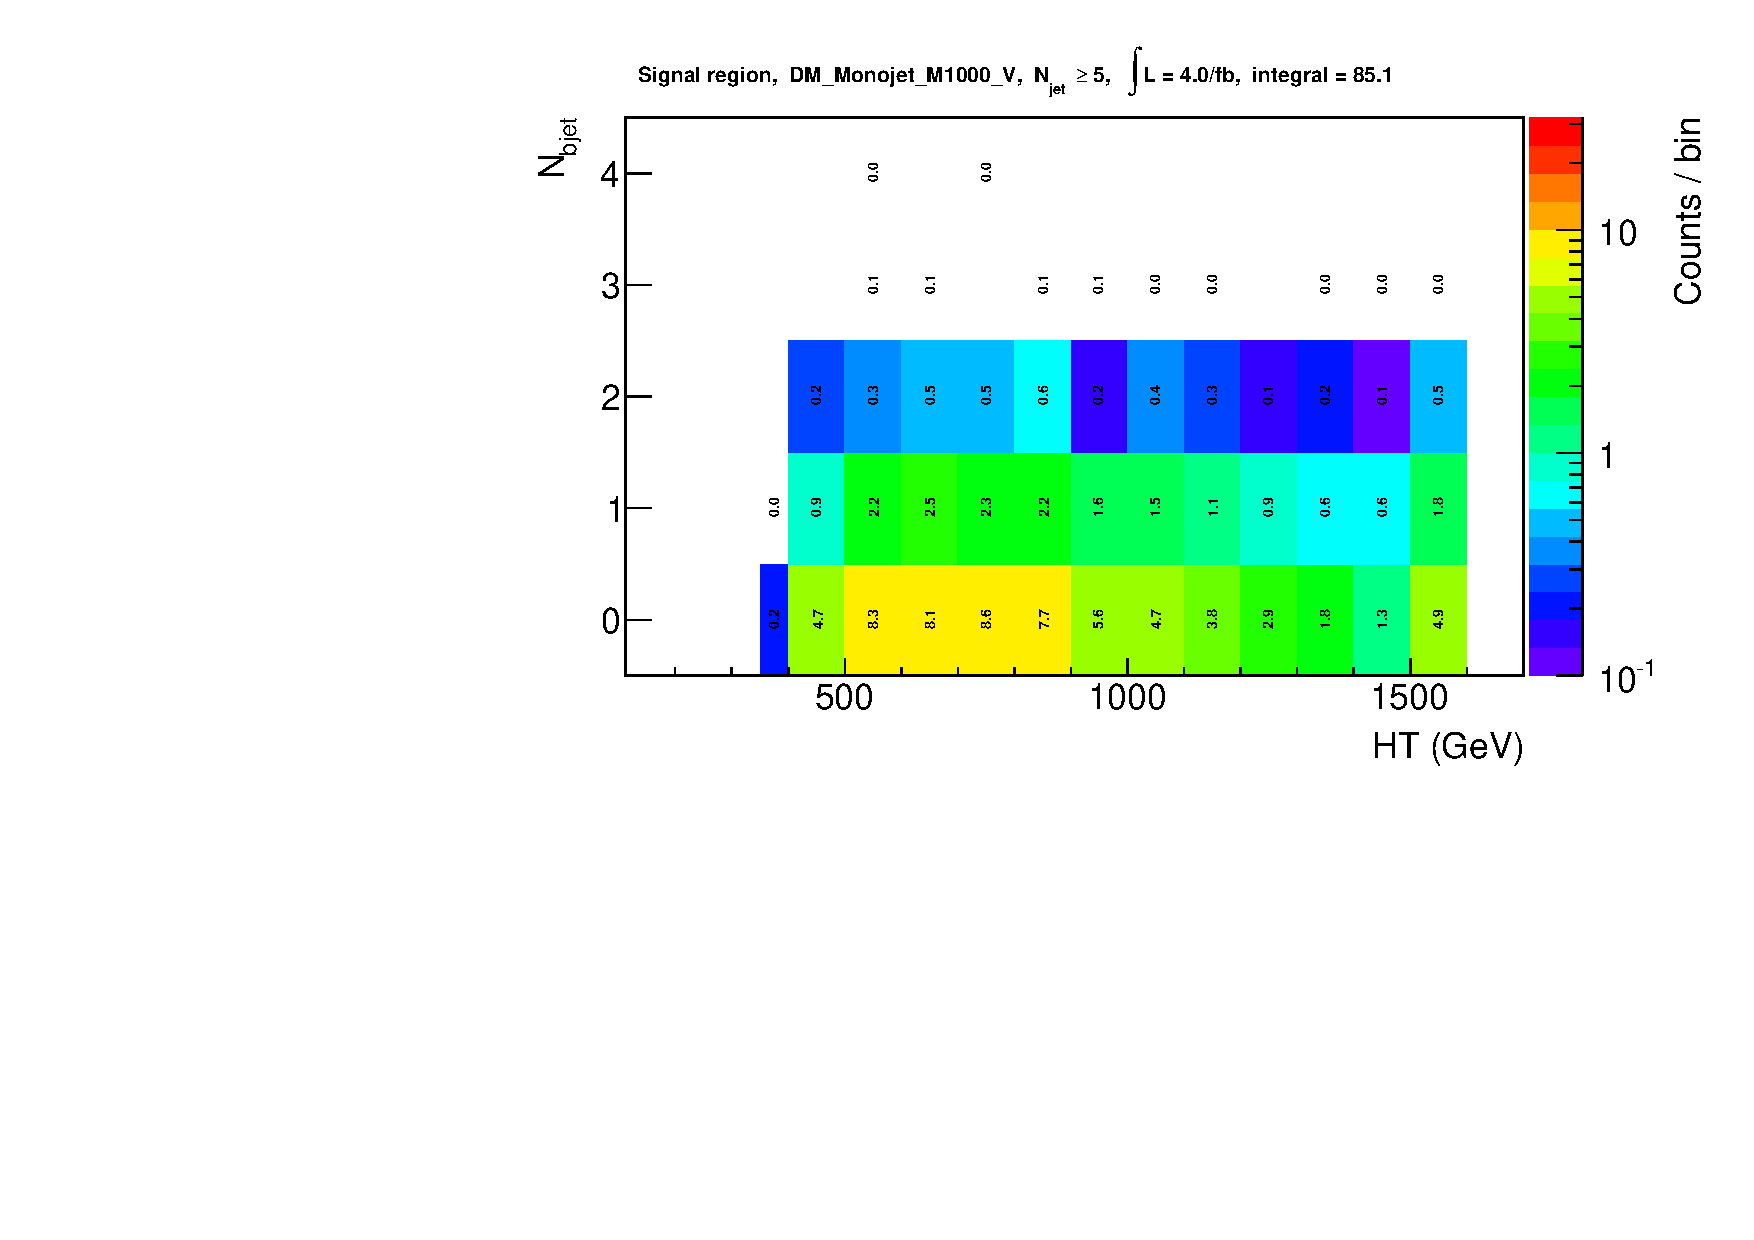
\includegraphics[width=0.5\textwidth]{figures/yieldPlots/sig_DM_Monojet_M1000_V_ge5j.pdf}
  }~~
  \subfigure[Hadronic signal region yields for the axial vectorDM model, asymetric selection.
  ($\njet = 5$)]{
    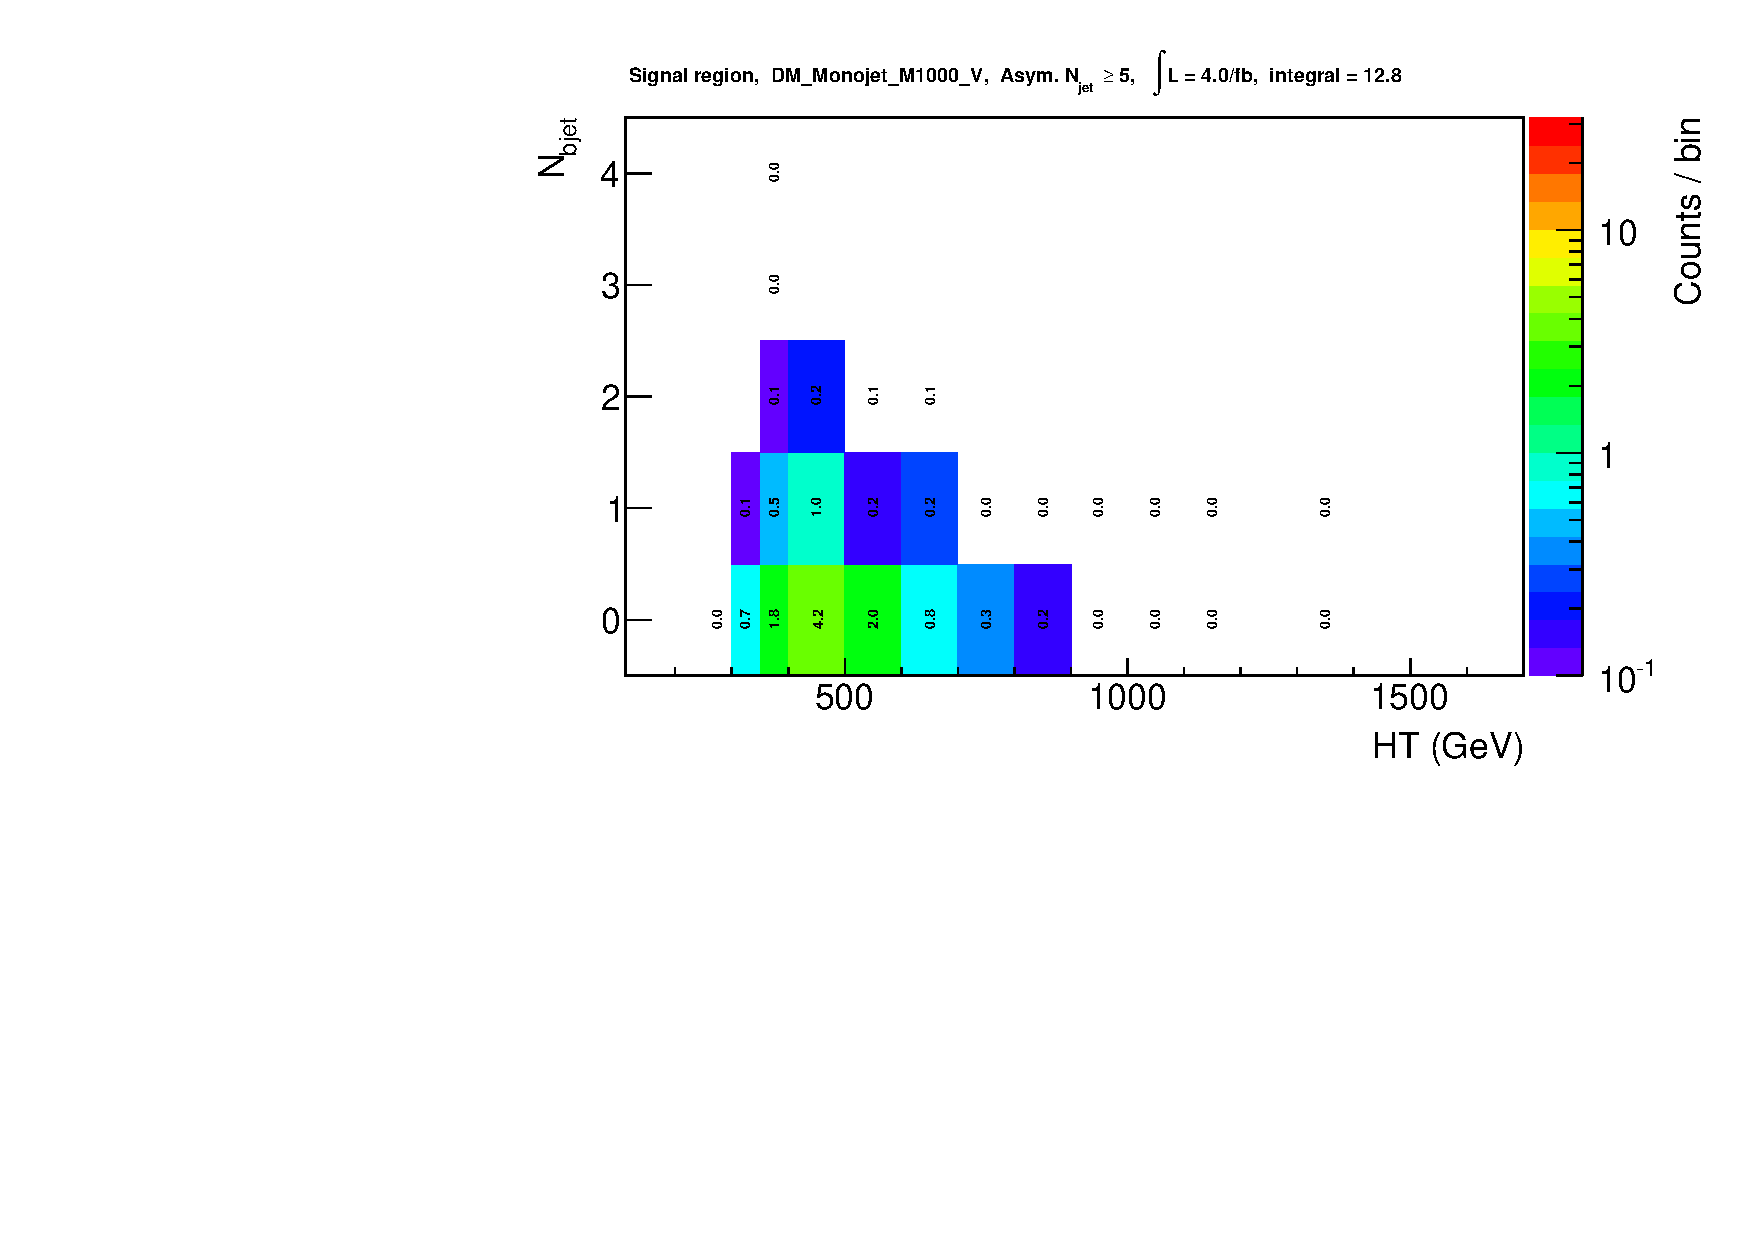
\includegraphics[width=0.5\textwidth]{figures/yieldPlots/sig_DM_Monojet_M1000_V_ge5jAsym.pdf}
  }
  \caption{\label{fig:DM_V_Yields2} Yields at $4\fbinv$ for the AV DM in the
  hadronic signal region, for $\njet=4,5$. The binning corresponds to the analysis  bins. }
\end{figure}







Corresponding figures for the $Tbbbb$ models are presented in Fig.\ref{fig:Tbbb_Yields2}.%~\ref{fig:Tbbb_Yields1}-~

%no point in showing these as there are no events

%\begin{figure}[]
%  \centering
%  \subfigure[Hadronic signal region yields for the axial vector DM model, nominal selection.
%  ($\njet = 2$)]{
%    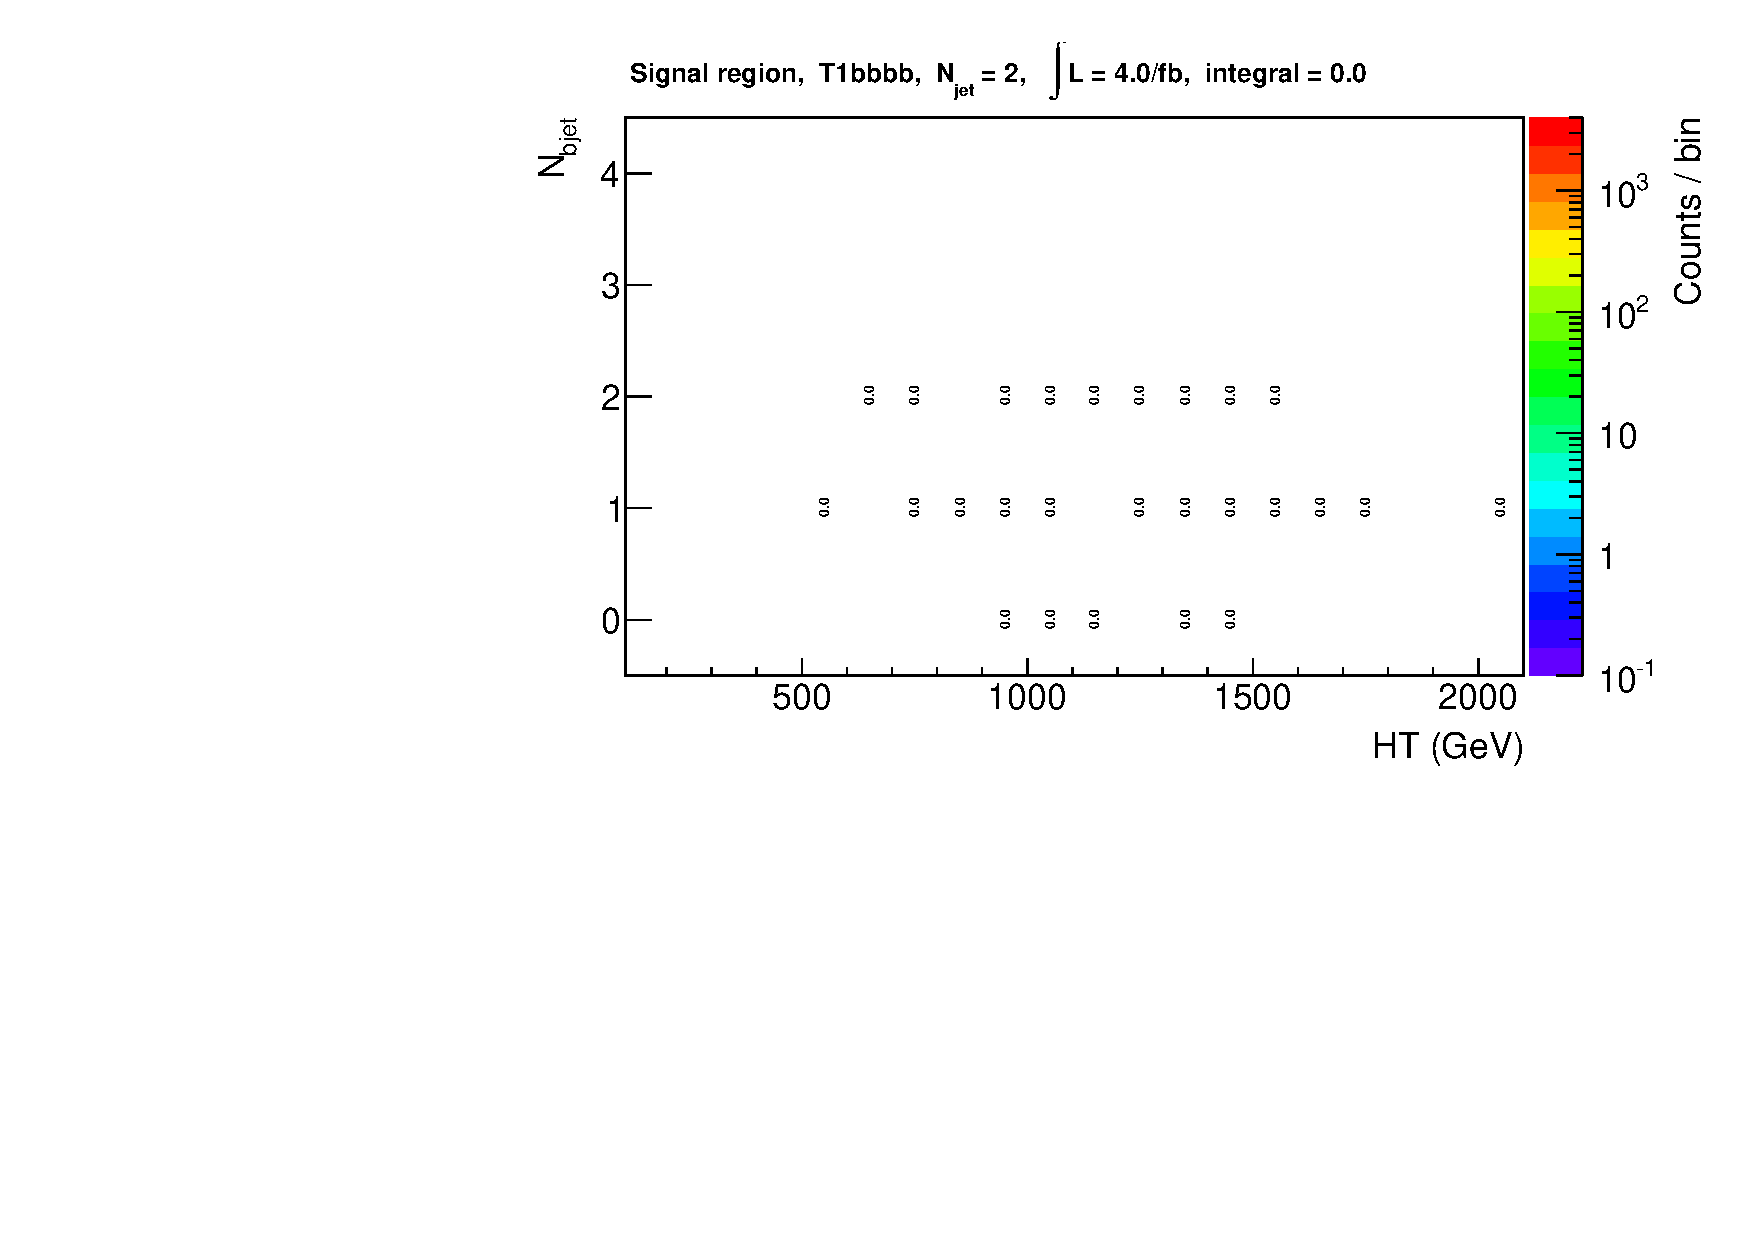
\includegraphics[width=0.5\textwidth]{figures/yieldPlots/sig_T1bbbb_eq2j.pdf}
%  }~~
%  \subfigure[Hadronic signal region yields for the axial vectorDM model, asymetric selection.
%  ($\njet = 2$)]{
%    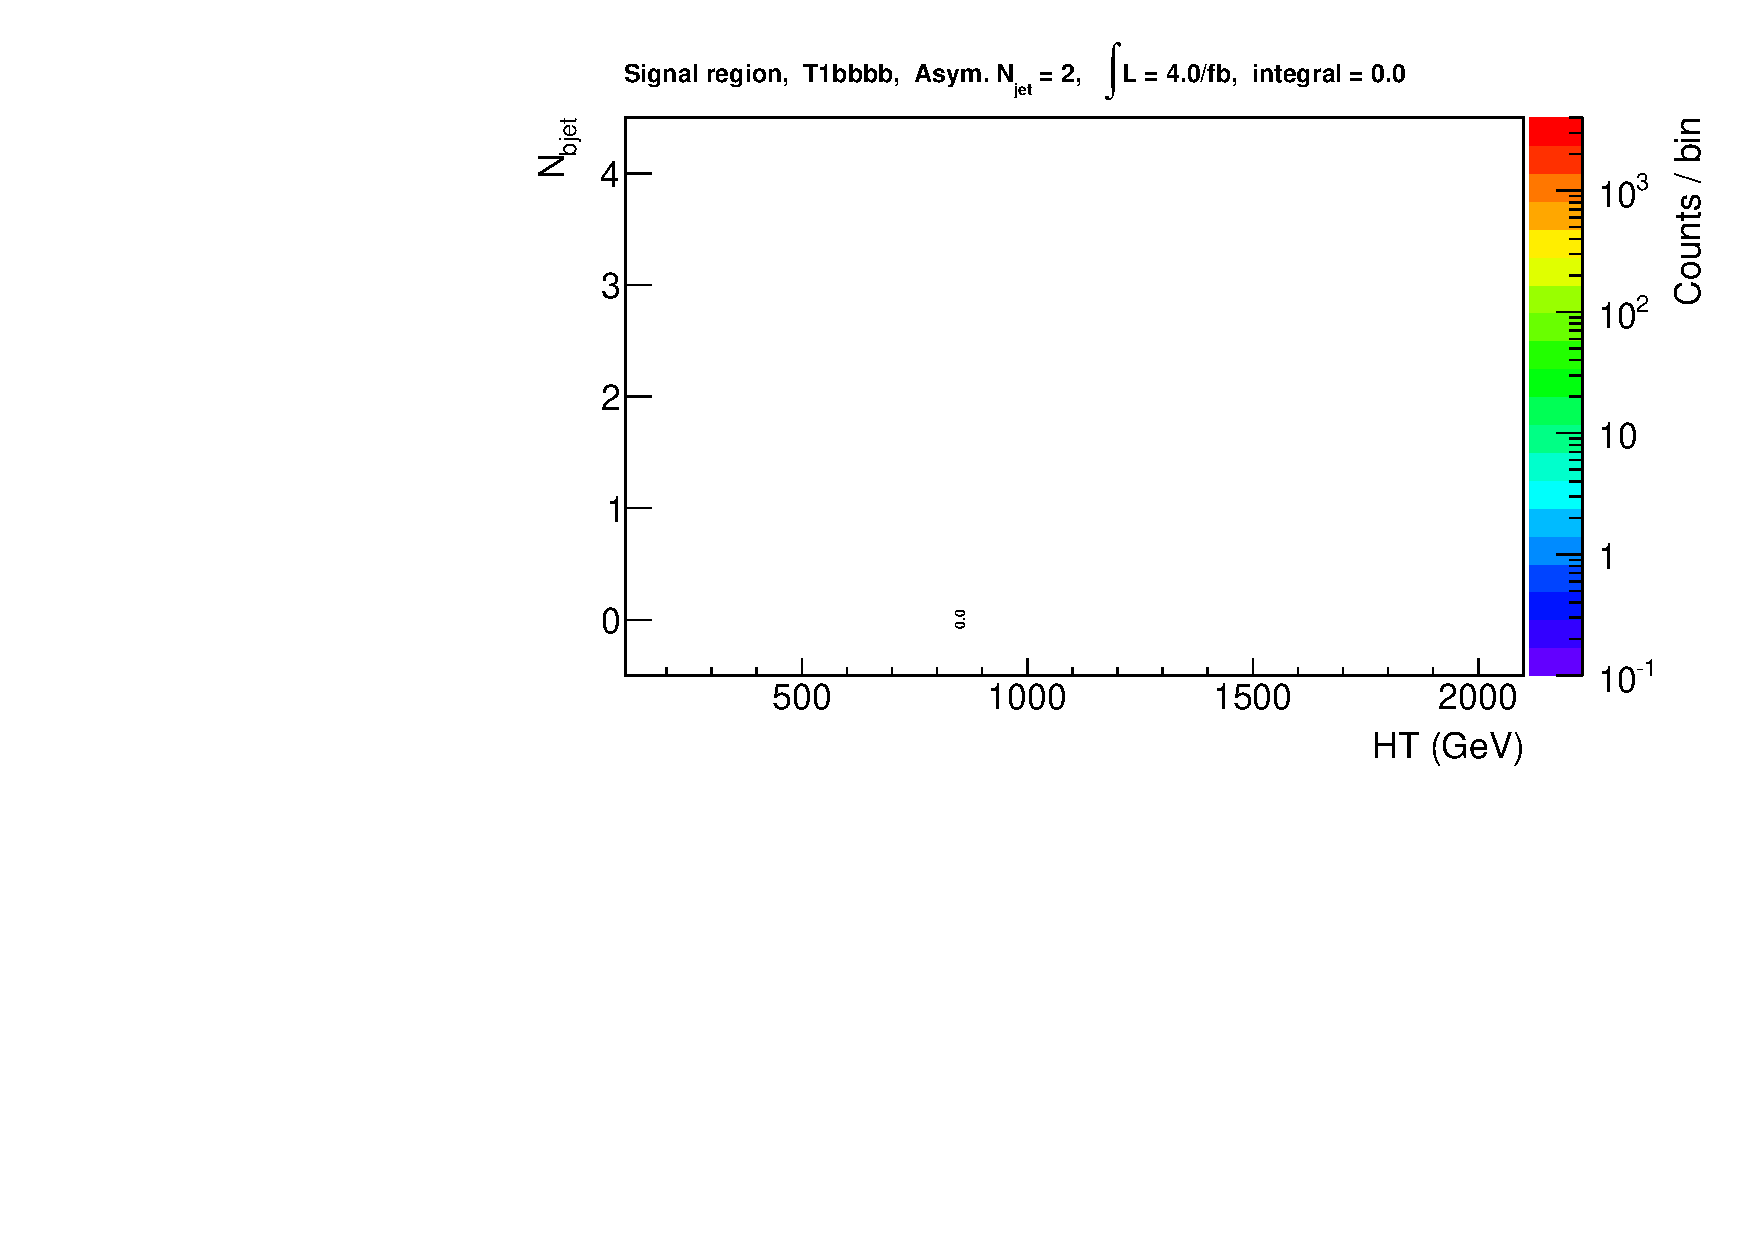
\includegraphics[width=0.5\textwidth]{figures/yieldPlots/sig_T1bbbb_eq2jAsym.pdf}
%  }\\
%
%  \subfigure[Hadronic signal region yields for the axial vector DM model, nominal selection.
%  ($\njet = 2$)]{
%    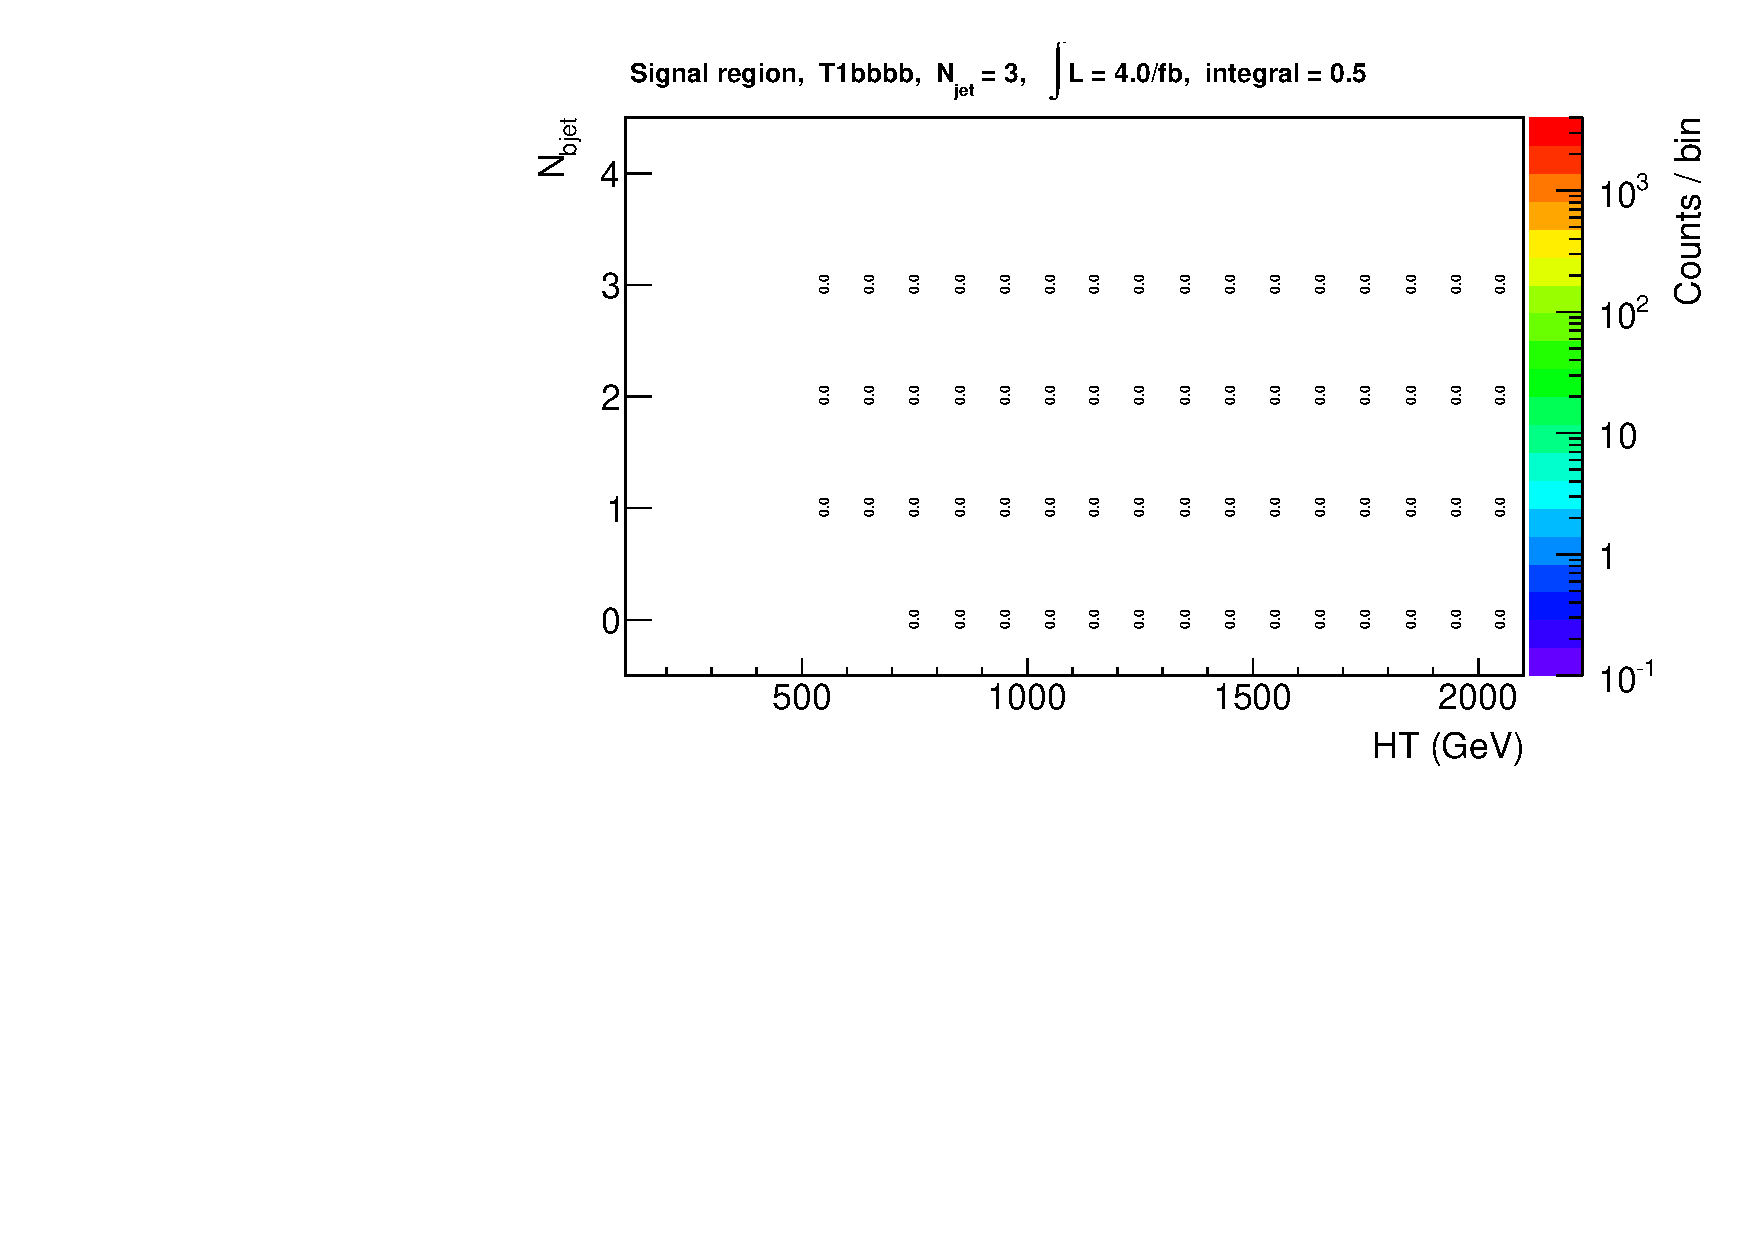
\includegraphics[width=0.5\textwidth]{figures/yieldPlots/sig_T1bbbb_eq3j.pdf}
%  }~~
%  \subfigure[Hadronic signal region yields for the axial vectorDM model, asymetric selection.
%  ($\njet = 2$)]{
%    \includegraphics[width=0.5\textwidth]{figures/yieldPlots/sig_T1bbbb_eq3jAsym.pdf}
%  }\\
%  \caption{\label{fig:Tbbb_Yields1} Yields at $4\fbinv$ for the $Tbbbb$ model in the
%  hadronic signal region, for $\njet=2,3$. The binning corresponds to the analysis  bins. }
%\end{figure}



\begin{figure}[]
  \centering
  \subfigure[Hadronic signal region yields for the T1bbbb simplified model, nominal selection.
  ($\njet = 4$)]{
    \includegraphics[width=0.5\textwidth]{figures/yieldPlots/sig_T1bbbb_eq4j.pdf}
  }~~
  \subfigure[Hadronic signal region yields for the T1bbbb simplified model, asymetric selection.
  ($\njet = 4$)]{
    \includegraphics[width=0.5\textwidth]{figures/yieldPlots/sig_T1bbbb_eq4jAsym.pdf}
  }\\

  \subfigure[Hadronic signal region yields for the T1bbbb simplified model, nominal selection.
  ($\njet \geq 5$)]{
    \includegraphics[width=0.5\textwidth]{figures/yieldPlots/sig_T1bbbb_ge5j.pdf}
  }~~
  \subfigure[Hadronic signal region yields for the T1bbbb simplified model, asymetric selection.
  ($\njet \geq 5$)]{
    \includegraphics[width=0.5\textwidth]{figures/yieldPlots/sig_T1bbbb_ge5jAsym.pdf}
  }
  \caption{\label{fig:Tbbb_Yields2} Yields at $4\fbinv$ for the $T1bbbb$ in the
  hadronic signal region, for $\njet=4,5$. The binning corresponds to the analysis  bins. }
\end{figure}




\clearpage

%%____________________________________________________________________________||


%%____________________________________________________________________________||
\subsection{Background yields for the asymmetric selection}


As in Sec.~\ref{sec:bkgd-comp} the yields are also assessed for the asymetric jet selection.
The plots presenting the yields for the electroweak backgrounds can be found in in Figs~\ref{fig:ewkYields1}-\ref{fig:ewkYields4}. 
The breakdown of the three dominant background processes,\zInv , \ttbar and $W+\textrm{jets}$, are also presented. 
Other background processes like single top and diboson processes, is found to be negligible and are therefore not 
shown.

\begin{figure}[]
  \centering
  \subfigure[Hadronic signal region yields for electroweak backgrounds
  ($\njet = 2$)]{
    \includegraphics[width=0.5\textwidth]{figures/yieldPlots/had_ewk_eq2jAsym.pdf}
  }~~
  \subfigure[Hadronic signal region yields for the \zInv background
  ($\njet = 2$)]{
    \includegraphics[width=0.5\textwidth]{figures/yieldPlots/had_zinv_eq2jAsym.pdf}
  }\\
  \subfigure[Hadronic signal region yields for W~+~jets backtround
  ($\njet = 2$)]{
    \includegraphics[width=0.5\textwidth]{figures/yieldPlots/had_wjets_eq2jAsym.pdf}
  }~~
  \subfigure[Hadronic signal region yields for \ttbar background
  ($\njet = 2$)]{
    \includegraphics[width=0.5\textwidth]{figures/yieldPlots/had_ttbar_eq2jAsym.pdf}
  }
  \caption{\label{fig:ewkYields1} Yields at $4\fbinv$ for the electroweak backgrounds in the
  hadronic signal region, $\njet=2$. The binning is chosen to be in line with the analysis
  bins. The contribution from the dominant backgrounds is shown separately.}
\end{figure}
\begin{figure}[]
  \centering
  \subfigure[Hadronic signal region yields for electroweak backgrounds
  ($\njet = 3$)]{
    \includegraphics[width=0.5\textwidth]{figures/yieldPlots/had_ewk_eq3jAsym.pdf}
  }~~
  \subfigure[Hadronic signal region yields for the \zInv background
  ($\njet = 3$)]{
    \includegraphics[width=0.5\textwidth]{figures/yieldPlots/had_zInv_eq3jAsym.pdf}
  }\\
  \subfigure[Hadronic signal region yields for W~+~jets backtround
  ($\njet = 3$)]{
    \includegraphics[width=0.5\textwidth]{figures/yieldPlots/had_wjets_eq3jAsym.pdf}
  }~~
  \subfigure[Hadronic signal region yields for \ttbar background
  ($\njet = 3$)]{
    \includegraphics[width=0.5\textwidth]{figures/yieldPlots/had_ttbar_eq3jAsym.pdf}
  }
  \caption{\label{fig:ewkYields2} Yields at $4\fbinv$ for the electroweak backgrounds in the
  hadronic signal region, $\njet=3$. The binning is chosen to be in line with the analysis
  bins. The contribution from the dominant backgrounds is shown separately.}
\end{figure}
\begin{figure}[]
  \centering
  \subfigure[Hadronic signal region yields for electroweak backgrounds
  ($\njet = 4$)]{
    \includegraphics[width=0.5\textwidth]{figures/yieldPlots/had_ewk_eq4jAsym.pdf}
  }~~
  \subfigure[Hadronic signal region yields for the \zInv background
  ($\njet = 4$)]{
    \includegraphics[width=0.5\textwidth]{figures/yieldPlots/had_zinv_eq4jAsym.pdf}
  }\\
  \subfigure[Hadronic signal region yields for W~+~jets backtround
  ($\njet = 4$)]{
    \includegraphics[width=0.5\textwidth]{figures/yieldPlots/had_wjets_eq4jAsym.pdf}
  }~~
  \subfigure[Hadronic signal region yields for \ttbar background
  ($\njet = 4$)]{
    \includegraphics[width=0.5\textwidth]{figures/yieldPlots/had_ttbar_eq4jAsym.pdf}
  }
  \caption{\label{fig:ewkYields3} Yields at $4\fbinv$ for the electroweak backgrounds in the
  hadronic signal region, $\njet=4$. The binning is chosen to be in line with the analysis
  bins. The contribution from the dominant backgrounds is shown separately.}
\end{figure}
\begin{figure}[]
  \centering
  \subfigure[Hadronic signal region yields for electroweak backgrounds
  ($\njet \geq 5$)]{
    \includegraphics[width=0.5\textwidth]{figures/yieldPlots/had_ewk_ge5jAsym.pdf}
  } ~~
  \subfigure[Hadronic signal region yields for the \zInv background
  ($\njet \geq 5$)]{
    \includegraphics[width=0.5\textwidth]{figures/yieldPlots/had_zinv_ge5jAsym.pdf}
  }\\
  \subfigure[Hadronic signal region yields for W~+~jets backtround
  ($\njet \geq 5$)]{
    \includegraphics[width=0.5\textwidth]{figures/yieldPlots/had_wjets_ge5jAsym.pdf}
  }~~
  \subfigure[Hadronic signal region yields for \ttbar background
  ($\njet \geq 5$)]{
    \includegraphics[width=0.5\textwidth]{figures/yieldPlots/had_ttbar_ge5jAsym.pdf}
  }
  \caption{\label{fig:ewkYields4} Yields at $4\fbinv$ for the electroweak backgrounds in the
  hadronic signal region, $\njet\geq5$. The binning is chosen to be in line with the analysis
  bins. The contribution from the dominant backgrounds is shown separately.}
\end{figure}

%%____________________________________________________________________________||
\subsubsection{Background yields for control regions}

The yields in the \mj, \mmj and \gj control samples can be seen in
Figures~\ref{fig:muYields}, \ref{fig:mumuYields} and \ref{fig:gammaYields}
respectively. The number of events in each of these bins is important for
working out how far we can extend in our analysis bins. We require there to be
enough events in the control samples to allow robust data driven prediction of
the backgrounds.

\begin{figure}[h!]
  \centering
  \subfigure[Yields from \texorpdfstring{\mj}{muon plus jets} control sample
  ($\njet = 2$)]{
    \includegraphics[width=0.5\textwidth]{figures/yieldPlots/mu_ewk_eq2jAsym.pdf}
  }~~
  \subfigure[Yields from \texorpdfstring{\mj}{muon plus jets} control sample
  ($\njet = 3$)]{
    \includegraphics[width=0.5\textwidth]{figures/yieldPlots/mu_ewk_eq3jAsym.pdf}
  }
  \\
  \subfigure[Yields from \texorpdfstring{\mj}{muon plus jets} control sample
  ($\njet = 4$)]{
    \includegraphics[width=0.5\textwidth]{figures/yieldPlots/mu_ewk_eq4jAsym.pdf}
  }~~
  \subfigure[Yields from \texorpdfstring{\mj}{muon plus jets} control sample
  ($\njet \geq 5$)]{
    \includegraphics[width=0.5\textwidth]{figures/yieldPlots/mu_ewk_ge5jAsym.pdf}
  } 
  \\
  \caption{\label{fig:muYields} Yields at $4\fbinv$ for the W~+~jets and \ttbar
  MC contributions to the \texorpdfstring{\mj}{muon plus jets} control sample. }
\end{figure}

\begin{figure}[h!]
  \centering
  \subfigure[Yields from \texorpdfstring{\mmj}{di-muon plus jets} control sample
  ($\njet = 2$)]{
    \includegraphics[width=0.5\textwidth]{figures/yieldPlots/mm_dy_eq2jAsym.pdf}
  }~~
  \subfigure[Yields from \texorpdfstring{\mmj}{di-muon plus jets} control sample
  ($\njet = 3$)]{
    \includegraphics[width=0.5\textwidth]{figures/yieldPlots/mm_dy_eq3jAsym.pdf}
  }
  \\
  \subfigure[Yields from \texorpdfstring{\mmj}{di-muon plus jets} control sample
  ($\njet = 4$)]{
    \includegraphics[width=0.5\textwidth]{figures/yieldPlots/mm_dy_eq4jAsym.pdf}
  }~~
  \subfigure[Yields from \texorpdfstring{\mmj}{di-muon plus jets} control sample
  ($\njet \geq 5$)]{
    \includegraphics[width=0.5\textwidth]{figures/yieldPlots/mm_dy_ge5jAsym.pdf}
  } 
  \\
  \caption{\label{fig:mumuYields} Yields at $4\fbinv$ for the DY~+~jets MC 
  contributions to the \texorpdfstring{\mmj}{di-muon plus jets} control sample. }
\end{figure}

\begin{figure}[h!]
  \centering
  \subfigure[Yields from \texorpdfstring{\gj}{photon plus jets} control sample
  ($\njet = 2$)]{
    \includegraphics[width=0.5\textwidth]{figures/yieldPlots/ph_gjets_eq2jAsym.pdf}
  }~~
  \subfigure[Yields from \texorpdfstring{\gj}{photon plus jets} control sample
  ($\njet = 3$)]{
    \includegraphics[width=0.5\textwidth]{figures/yieldPlots/ph_gjets_eq3jAsym.pdf}
  }
  \\
  \subfigure[Yields from \texorpdfstring{\gj}{photon plus jets} control sample
  ($\njet = 4$)]{
    \includegraphics[width=0.5\textwidth]{figures/yieldPlots/ph_gjets_eq4jAsym.pdf}
  }~~
  \subfigure[Yields from \texorpdfstring{\gj}{photon plus jets} control sample
  ($\njet \geq 5$)]{
    \includegraphics[width=0.5\textwidth]{figures/yieldPlots/ph_gjets_ge5jAsym.pdf}
  } 
  \\
  \caption{\label{fig:gammaYields} Yields at $4\fbinv$ for the GJets MC 
  contributions to the \texorpdfstring{\gj}{photon plus jets} control sample. }
\end{figure}


